% Options for packages loaded elsewhere
\PassOptionsToPackage{unicode}{hyperref}
\PassOptionsToPackage{hyphens}{url}
%
\documentclass[
]{article}
\usepackage{amsmath,amssymb}
\usepackage{iftex}
\ifPDFTeX
  \usepackage[T1]{fontenc}
  \usepackage[utf8]{inputenc}
  \usepackage{textcomp} % provide euro and other symbols
\else % if luatex or xetex
  \usepackage{unicode-math} % this also loads fontspec
  \defaultfontfeatures{Scale=MatchLowercase}
  \defaultfontfeatures[\rmfamily]{Ligatures=TeX,Scale=1}
\fi
\usepackage{lmodern}
\ifPDFTeX\else
  % xetex/luatex font selection
\fi
% Use upquote if available, for straight quotes in verbatim environments
\IfFileExists{upquote.sty}{\usepackage{upquote}}{}
\IfFileExists{microtype.sty}{% use microtype if available
  \usepackage[]{microtype}
  \UseMicrotypeSet[protrusion]{basicmath} % disable protrusion for tt fonts
}{}
\makeatletter
\@ifundefined{KOMAClassName}{% if non-KOMA class
  \IfFileExists{parskip.sty}{%
    \usepackage{parskip}
  }{% else
    \setlength{\parindent}{0pt}
    \setlength{\parskip}{6pt plus 2pt minus 1pt}}
}{% if KOMA class
  \KOMAoptions{parskip=half}}
\makeatother
\usepackage{xcolor}
\usepackage[margin=1in]{geometry}
\usepackage{color}
\usepackage{fancyvrb}
\newcommand{\VerbBar}{|}
\newcommand{\VERB}{\Verb[commandchars=\\\{\}]}
\DefineVerbatimEnvironment{Highlighting}{Verbatim}{commandchars=\\\{\}}
% Add ',fontsize=\small' for more characters per line
\usepackage{framed}
\definecolor{shadecolor}{RGB}{248,248,248}
\newenvironment{Shaded}{\begin{snugshade}}{\end{snugshade}}
\newcommand{\AlertTok}[1]{\textcolor[rgb]{0.94,0.16,0.16}{#1}}
\newcommand{\AnnotationTok}[1]{\textcolor[rgb]{0.56,0.35,0.01}{\textbf{\textit{#1}}}}
\newcommand{\AttributeTok}[1]{\textcolor[rgb]{0.13,0.29,0.53}{#1}}
\newcommand{\BaseNTok}[1]{\textcolor[rgb]{0.00,0.00,0.81}{#1}}
\newcommand{\BuiltInTok}[1]{#1}
\newcommand{\CharTok}[1]{\textcolor[rgb]{0.31,0.60,0.02}{#1}}
\newcommand{\CommentTok}[1]{\textcolor[rgb]{0.56,0.35,0.01}{\textit{#1}}}
\newcommand{\CommentVarTok}[1]{\textcolor[rgb]{0.56,0.35,0.01}{\textbf{\textit{#1}}}}
\newcommand{\ConstantTok}[1]{\textcolor[rgb]{0.56,0.35,0.01}{#1}}
\newcommand{\ControlFlowTok}[1]{\textcolor[rgb]{0.13,0.29,0.53}{\textbf{#1}}}
\newcommand{\DataTypeTok}[1]{\textcolor[rgb]{0.13,0.29,0.53}{#1}}
\newcommand{\DecValTok}[1]{\textcolor[rgb]{0.00,0.00,0.81}{#1}}
\newcommand{\DocumentationTok}[1]{\textcolor[rgb]{0.56,0.35,0.01}{\textbf{\textit{#1}}}}
\newcommand{\ErrorTok}[1]{\textcolor[rgb]{0.64,0.00,0.00}{\textbf{#1}}}
\newcommand{\ExtensionTok}[1]{#1}
\newcommand{\FloatTok}[1]{\textcolor[rgb]{0.00,0.00,0.81}{#1}}
\newcommand{\FunctionTok}[1]{\textcolor[rgb]{0.13,0.29,0.53}{\textbf{#1}}}
\newcommand{\ImportTok}[1]{#1}
\newcommand{\InformationTok}[1]{\textcolor[rgb]{0.56,0.35,0.01}{\textbf{\textit{#1}}}}
\newcommand{\KeywordTok}[1]{\textcolor[rgb]{0.13,0.29,0.53}{\textbf{#1}}}
\newcommand{\NormalTok}[1]{#1}
\newcommand{\OperatorTok}[1]{\textcolor[rgb]{0.81,0.36,0.00}{\textbf{#1}}}
\newcommand{\OtherTok}[1]{\textcolor[rgb]{0.56,0.35,0.01}{#1}}
\newcommand{\PreprocessorTok}[1]{\textcolor[rgb]{0.56,0.35,0.01}{\textit{#1}}}
\newcommand{\RegionMarkerTok}[1]{#1}
\newcommand{\SpecialCharTok}[1]{\textcolor[rgb]{0.81,0.36,0.00}{\textbf{#1}}}
\newcommand{\SpecialStringTok}[1]{\textcolor[rgb]{0.31,0.60,0.02}{#1}}
\newcommand{\StringTok}[1]{\textcolor[rgb]{0.31,0.60,0.02}{#1}}
\newcommand{\VariableTok}[1]{\textcolor[rgb]{0.00,0.00,0.00}{#1}}
\newcommand{\VerbatimStringTok}[1]{\textcolor[rgb]{0.31,0.60,0.02}{#1}}
\newcommand{\WarningTok}[1]{\textcolor[rgb]{0.56,0.35,0.01}{\textbf{\textit{#1}}}}
\usepackage{graphicx}
\makeatletter
\def\maxwidth{\ifdim\Gin@nat@width>\linewidth\linewidth\else\Gin@nat@width\fi}
\def\maxheight{\ifdim\Gin@nat@height>\textheight\textheight\else\Gin@nat@height\fi}
\makeatother
% Scale images if necessary, so that they will not overflow the page
% margins by default, and it is still possible to overwrite the defaults
% using explicit options in \includegraphics[width, height, ...]{}
\setkeys{Gin}{width=\maxwidth,height=\maxheight,keepaspectratio}
% Set default figure placement to htbp
\makeatletter
\def\fps@figure{htbp}
\makeatother
\setlength{\emergencystretch}{3em} % prevent overfull lines
\providecommand{\tightlist}{%
  \setlength{\itemsep}{0pt}\setlength{\parskip}{0pt}}
\setcounter{secnumdepth}{-\maxdimen} % remove section numbering
\usepackage{booktabs}
\usepackage{longtable}
\usepackage{array}
\usepackage{multirow}
\usepackage{wrapfig}
\usepackage{float}
\usepackage{colortbl}
\usepackage{pdflscape}
\usepackage{tabu}
\usepackage{threeparttable}
\usepackage{threeparttablex}
\usepackage[normalem]{ulem}
\usepackage{makecell}
\usepackage{xcolor}
\ifLuaTeX
  \usepackage{selnolig}  % disable illegal ligatures
\fi
\IfFileExists{bookmark.sty}{\usepackage{bookmark}}{\usepackage{hyperref}}
\IfFileExists{xurl.sty}{\usepackage{xurl}}{} % add URL line breaks if available
\urlstyle{same}
\hypersetup{
  pdftitle={TMA4315 Generalized linear models H2018},
  pdfauthor={Mette Langaas, Department of Mathematical Sciences, NTNU -- with contributions from Oyvind Bakke and Ingeborg Hem},
  hidelinks,
  pdfcreator={LaTeX via pandoc}}

\title{TMA4315 Generalized linear models H2018}
\usepackage{etoolbox}
\makeatletter
\providecommand{\subtitle}[1]{% add subtitle to \maketitle
  \apptocmd{\@title}{\par {\large #1 \par}}{}{}
}
\makeatother
\subtitle{Module 2: MULTIPLE LINEAR REGRESSION}
\author{Mette Langaas, Department of Mathematical Sciences, NTNU -- with
contributions from Oyvind Bakke and Ingeborg Hem}
\date{30.08 and 06.09 {[}PL{]}, 31.08 and 07.09 {[}IL{]}}

\begin{document}
\maketitle

{
\setcounter{tocdepth}{2}
\tableofcontents
}
(Latest changes: 09.12 Typos from Scott. 05.09.2018. Typos and added
wordcloud code.)

\hypertarget{overview}{%
\section{Overview}\label{overview}}

\hypertarget{learning-material}{%
\subsection{Learning material}\label{learning-material}}

\begin{itemize}
\tightlist
\item
  Textbook: Chapter 2.2, 3 and B.4. (Chapter 3 was on the reading list
  for TMA4267 Linear statistical 2016-2018, so much of this module is
  know from before - but not from a GLM point of view!)
\item
  \href{https://www.math.ntnu.no/emner/TMA4315/2018h/TMA4315M2H20180830.pdf}{Classnotes
  30.08.2018}
\item
  \href{https://www.math.ntnu.no/emner/TMA4315/2018h/TMA4315M2H20180906.pdf}{Classnotes
  06.09.2018}
\end{itemize}

\begin{center}\rule{0.5\linewidth}{0.5pt}\end{center}

\hypertarget{topics}{%
\subsection{Topics}\label{topics}}

\hypertarget{first-week}{%
\subsubsection{\texorpdfstring{\protect\hyperlink{firstweek}{First
week}}{First week}}\label{first-week}}

\begin{itemize}
\tightlist
\item
  Aim of multiple linear regression.
\item
  Define and understand the multiple linear regression model -
  traditional and GLM way
\item
  parameter estimation with maximum likelihood (and least squares),
\item
  likelihood, score vector and Hessian (observed Fisher information
  matrix)
\item
  properties of parameter estimators,
\item
  assessing model fit (diagnostic), residuals, QQ-plots,
\item
  design matrix: how to code categorical covariates (dummy or effect
  coding), and how to handle interactions.
\end{itemize}

Jump to \protect\hyperlink{interactivew1}{IL for first week}

\begin{center}\rule{0.5\linewidth}{0.5pt}\end{center}

\hypertarget{second-week}{%
\subsubsection{\texorpdfstring{\protect\hyperlink{secondweek}{Second
week}}{Second week}}\label{second-week}}

\begin{itemize}
\tightlist
\item
  What did we do last week?
\item
  Parameter estimation in practice.
\item
  Statistical inference for parameter estimates

  \begin{itemize}
  \tightlist
  \item
    confidence intervals,
  \item
    prediction intervals,
  \item
    hypothesis test,
  \item
    linear hypotheses.
  \end{itemize}
\item
  Introducing deviance - and likelihood ratio test
\item
  Analysis of variance decompositions and \(R^2\), sequential ANOVA
  table.
\item
  Model selection with AIC
\end{itemize}

Jump to \protect\hyperlink{secondweek}{second week} and
\protect\hyperlink{interactivew2}{IL for second week}

\textbf{FIRST WEEK}

\hypertarget{aim-of-multiple-linear-regression}{%
\section{Aim of multiple linear
regression}\label{aim-of-multiple-linear-regression}}

\begin{enumerate}
\def\labelenumi{\arabic{enumi}.}
\item
  Construct a model to help understand the relationship between a
  response and one or several explanatory variables. {[}Correlation, or
  cause and effect?{]}
\item
  Construct a model to predict the reponse from a set of (one or
  several) explanatory variables. {[}More or less ``black box''{]}
\end{enumerate}

\begin{center}\rule{0.5\linewidth}{0.5pt}\end{center}

\hypertarget{munich-rent-index}{%
\subsubsection{Munich rent index}\label{munich-rent-index}}

Munich, 1999: 3082 observations on 9 variables.

\begin{itemize}
\tightlist
\item
  \texttt{rent}: the net rent per month (in Euro).
\item
  \texttt{rentsqm}: the net rent per month per square meter (in Euro).
\item
  \texttt{area}: living area in square meters.
\item
  \texttt{yearc}: year of construction.
\item
  \texttt{location}: quality of location: a factor indicating whether
  the location is average location, 1, good location, 2, and top
  location, 3.
\item
  \texttt{bath}: quality of bathroom: a a factor indicating whether the
  bath facilities are standard, 0, or premium, 1.
\item
  \texttt{kitchen}: Quality of kitchen: 0 standard 1 premium.
\item
  \texttt{cheating}: central heating: a factor 0 without central
  heating, 1 with central heating.
\item
  \texttt{district}: District in Munich.
\end{itemize}

More information in Fahrmeir et. al., (2013) page 5.

\begin{center}\rule{0.5\linewidth}{0.5pt}\end{center}

\footnotesize

\begin{Shaded}
\begin{Highlighting}[]
\FunctionTok{library}\NormalTok{(}\StringTok{"gamlss.data"}\NormalTok{)}
\FunctionTok{library}\NormalTok{(GGally)}
\FunctionTok{ggpairs}\NormalTok{(rent99, }\AttributeTok{lower =} \FunctionTok{list}\NormalTok{(}\AttributeTok{combo =} \FunctionTok{wrap}\NormalTok{(ggally\_facethist, }\AttributeTok{binwidth =} \FloatTok{0.5}\NormalTok{)))}
\end{Highlighting}
\end{Shaded}

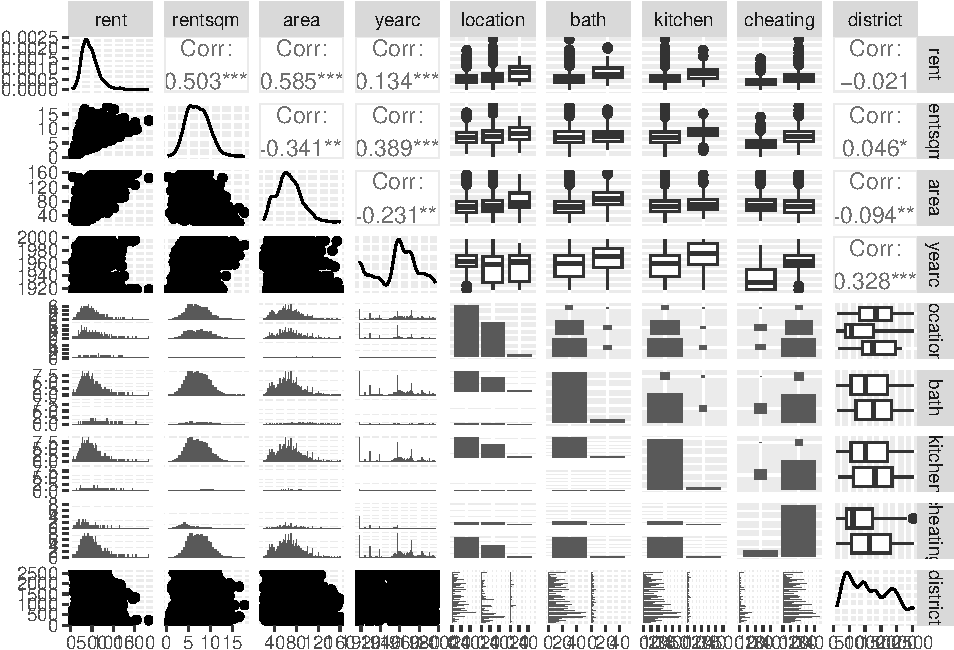
\includegraphics{2MLR_files/figure-latex/unnamed-chunk-1-1.pdf}
\normalsize

\begin{center}\rule{0.5\linewidth}{0.5pt}\end{center}

\textbf{Interesting questions}

\begin{enumerate}
\def\labelenumi{\arabic{enumi}.}
\tightlist
\item
  Is there a relationship between \texttt{rent} and \texttt{area}?
\item
  How strong is this relationship?
\item
  Is the relationship linear?
\item
  Are also other variables associated with \texttt{rent}?
\item
  How well can we predict the rent of an appartment?
\item
  Is the effect of \texttt{area} the same on \texttt{rent} for
  appartments at average, good and top \texttt{location}? (interaction)
\end{enumerate}

\begin{center}\rule{0.5\linewidth}{0.5pt}\end{center}

\hypertarget{notation}{%
\section{Notation}\label{notation}}

\begin{center}\rule{0.5\linewidth}{0.5pt}\end{center}

\({\bf Y}: (n \times 1)\) vector of responses (random variable)
{[}e.g.~one of the following: rent, rent pr sqm, weight of baby, ph of
lake, volume of tree{]}

\({\bf X}: (n \times p)\) design matrix {[}e.g.~location of flat,
gestation age of baby, chemical measurement of the lake, height of
tree{]}

\({\bf \boldsymbol{\beta}}: (p \times 1)\) vector of regression
parameters (intercept included, so \(p=k+1\))

\({\bf \varepsilon}: (n\times 1)\) vector of random errors. Used in
``traditional way''.

We assume that pairs \(({\bf x}_i^T,y_i)\) (\(i=1,...,n\)) are measured
from sampling units. That is, the observation pair \(({\bf x}_1^T,y_1)\)
is independent from \(({\bf x}_2^T,y_2)\), and so on.

\begin{center}\rule{0.5\linewidth}{0.5pt}\end{center}

\hypertarget{hands-on-munich-rent-index-response-and-covariates}{%
\subsubsection{Hands on: Munich rent index --- response and
covariates}\label{hands-on-munich-rent-index-response-and-covariates}}

Study the print-out and discuss the following questions:

\begin{enumerate}
\def\labelenumi{\alph{enumi})}
\tightlist
\item
  What can be response, and what covariates? (using what you know about
  rents)
\item
  What type of response(s) do we have? (continuous, categorical,
  nominal, ordinal, discrete, factors, \ldots).
\item
  What types of covariates? (continuous, categorical, nominal, ordinal,
  discrete, factors, \ldots)
\item
  Explain what the elements of \texttt{model.matrix} are. (Hint: coding
  of \texttt{location})
\end{enumerate}

\begin{center}\rule{0.5\linewidth}{0.5pt}\end{center}

\begin{Shaded}
\begin{Highlighting}[]
\FunctionTok{library}\NormalTok{(}\StringTok{"gamlss.data"}\NormalTok{)}
\NormalTok{ds }\OtherTok{=}\NormalTok{ rent99}
\FunctionTok{colnames}\NormalTok{(ds)}
\end{Highlighting}
\end{Shaded}

\begin{verbatim}
## [1] "rent"     "rentsqm"  "area"     "yearc"    "location" "bath"     "kitchen" 
## [8] "cheating" "district"
\end{verbatim}

\begin{Shaded}
\begin{Highlighting}[]
\FunctionTok{summary}\NormalTok{(ds)}
\end{Highlighting}
\end{Shaded}

\begin{verbatim}
##       rent            rentsqm             area            yearc      location
##  Min.   :  40.51   Min.   : 0.4158   Min.   : 20.00   Min.   :1918   1:1794  
##  1st Qu.: 322.03   1st Qu.: 5.2610   1st Qu.: 51.00   1st Qu.:1939   2:1210  
##  Median : 426.97   Median : 6.9802   Median : 65.00   Median :1959   3:  78  
##  Mean   : 459.44   Mean   : 7.1113   Mean   : 67.37   Mean   :1956           
##  3rd Qu.: 559.36   3rd Qu.: 8.8408   3rd Qu.: 81.00   3rd Qu.:1972           
##  Max.   :1843.38   Max.   :17.7216   Max.   :160.00   Max.   :1997           
##  bath     kitchen  cheating    district   
##  0:2891   0:2951   0: 321   Min.   : 113  
##  1: 191   1: 131   1:2761   1st Qu.: 561  
##                             Median :1025  
##                             Mean   :1170  
##                             3rd Qu.:1714  
##                             Max.   :2529
\end{verbatim}

\begin{Shaded}
\begin{Highlighting}[]
\FunctionTok{dim}\NormalTok{(ds)}
\end{Highlighting}
\end{Shaded}

\begin{verbatim}
## [1] 3082    9
\end{verbatim}

\begin{Shaded}
\begin{Highlighting}[]
\FunctionTok{head}\NormalTok{(ds)}
\end{Highlighting}
\end{Shaded}

\begin{verbatim}
##       rent   rentsqm area yearc location bath kitchen cheating district
## 1 109.9487  4.228797   26  1918        2    0       0        0      916
## 2 243.2820  8.688646   28  1918        2    0       0        1      813
## 3 261.6410  8.721369   30  1918        1    0       0        1      611
## 4 106.4103  3.547009   30  1918        2    0       0        0     2025
## 5 133.3846  4.446154   30  1918        2    0       0        1      561
## 6 339.0256 11.300851   30  1918        2    0       0        1      541
\end{verbatim}

\begin{Shaded}
\begin{Highlighting}[]
\FunctionTok{str}\NormalTok{(ds}\SpecialCharTok{$}\NormalTok{location)}
\end{Highlighting}
\end{Shaded}

\begin{verbatim}
##  Factor w/ 3 levels "1","2","3": 2 2 1 2 2 2 1 1 1 2 ...
\end{verbatim}

\begin{Shaded}
\begin{Highlighting}[]
\FunctionTok{contrasts}\NormalTok{(ds}\SpecialCharTok{$}\NormalTok{location)}
\end{Highlighting}
\end{Shaded}

\begin{verbatim}
##   2 3
## 1 0 0
## 2 1 0
## 3 0 1
\end{verbatim}

\begin{Shaded}
\begin{Highlighting}[]
\NormalTok{X }\OtherTok{=} \FunctionTok{model.matrix}\NormalTok{(rentsqm }\SpecialCharTok{\textasciitilde{}}\NormalTok{ area }\SpecialCharTok{+}\NormalTok{ yearc }\SpecialCharTok{+}\NormalTok{ location }\SpecialCharTok{+}\NormalTok{ bath }\SpecialCharTok{+}\NormalTok{ kitchen }\SpecialCharTok{+}
\NormalTok{    cheating }\SpecialCharTok{+}\NormalTok{ district, }\AttributeTok{data =}\NormalTok{ ds)}
\FunctionTok{head}\NormalTok{(X)}
\end{Highlighting}
\end{Shaded}

\begin{verbatim}
##   (Intercept) area yearc location2 location3 bath1 kitchen1 cheating1 district
## 1           1   26  1918         1         0     0        0         0      916
## 2           1   28  1918         1         0     0        0         1      813
## 3           1   30  1918         0         0     0        0         1      611
## 4           1   30  1918         1         0     0        0         0     2025
## 5           1   30  1918         1         0     0        0         1      561
## 6           1   30  1918         1         0     0        0         1      541
\end{verbatim}

\hypertarget{model}{%
\section{Model}\label{model}}

\begin{center}\rule{0.5\linewidth}{0.5pt}\end{center}

\hypertarget{the-traditional-way}{%
\subsection{The traditional way}\label{the-traditional-way}}

\[{\bf Y=X \boldsymbol{\beta}}+{\bf\varepsilon}\] is called a classical
linear model if the following is true:

\begin{enumerate}
\def\labelenumi{\arabic{enumi}.}
\item
  \(\text{E}(\bf{\varepsilon})=\bf{0}\).
\item
  \(\text{Cov}(\bf{\varepsilon})=\text{E}(\bf{\varepsilon}\bf{\varepsilon}^T)=\sigma^2\bf{I}\).
\item
  The design matrix has full rank, \(\text{rank}({\bf X})=k+1=p\).
\end{enumerate}

The classical \emph{normal} linear regression model is obtained if
additionally

\begin{enumerate}
\def\labelenumi{\arabic{enumi}.}
\setcounter{enumi}{3}
\tightlist
\item
  \(\varepsilon\sim N_n(\bf{0},\sigma^2\bf{I})\) holds.
\end{enumerate}

For random covariates these assumptions are to be understood
conditionally on \(\bf{X}\).

\begin{center}\rule{0.5\linewidth}{0.5pt}\end{center}

\hypertarget{the-glm-way}{%
\subsection{The GLM way}\label{the-glm-way}}

Independent pairs \((Y_i, {\bf x}_i)\) for \(i=1,\ldots,n\).

\begin{enumerate}
\def\labelenumi{\arabic{enumi}.}
\tightlist
\item
  Random component: \(Y_i \sim N\) with \(\text{E}(Y_i)=\mu_i\) and
  \(\text{Var}(Y_i)=\sigma^2\).
\item
  Systematic component: \(\eta_i={\bf x}_i^T \boldsymbol{\beta}\).
\item
  Link function: linking the random and systematic component (linear
  predictor): Identity link and response function. \(\mu_i=\eta_i\).
\end{enumerate}

\begin{center}\rule{0.5\linewidth}{0.5pt}\end{center}

\hypertarget{questions}{%
\subsubsection{Questions}\label{questions}}

\begin{itemize}
\tightlist
\item
  Compare the traditional and GLM way. Have we made the same assumptions
  for both?
\item
  What is the connection between each \({\bf x}_i\) and the design
  matrix?
\item
  What is ``full rank''? Why is this needed? Example of rank less than
  \(p\)?
\item
  Why do you think we move from traditional to GLM way? Could we not
  just let \(\varepsilon\) be from binomial, Poisson, etc. distribution?
\end{itemize}

\hypertarget{parameter-estimation}{%
\section{Parameter estimation}\label{parameter-estimation}}

In multiple linear regression there are two popular methods for
estimating the regression parameters in \(\boldsymbol{\beta}\): maximum
likelihood and least squares. These two methods give the same estimator
when we assume the normal linear regression model. We will in this
module focus on maximum likelihood estimation, since that can be used
also when we have non-normal responses (modules 3-6: binomial, Poisson,
gamma, multinomial).

\hypertarget{likelihood-theory-from-b.4}{%
\subsection{Likelihood theory (from
B.4)}\label{likelihood-theory-from-b.4}}

\begin{center}\rule{0.5\linewidth}{0.5pt}\end{center}

\hypertarget{likelihood-lboldsymbolbeta}{%
\subsubsection{\texorpdfstring{Likelihood
\(L(\boldsymbol{\beta})\)}{Likelihood L(\textbackslash boldsymbol\{\textbackslash beta\})}}\label{likelihood-lboldsymbolbeta}}

We assume that pairs of covariates and response are measured
independently of each other: \(({\bf x}_i,Y_i)\), and \(Y_i\) follows
the distribution specified above, and \({\bf x}_i\) is fixed.

\[L(\boldsymbol{\beta})=\prod_{i=1}^n L_i(\boldsymbol{\beta})=\prod_{i=1}^n f(y_i; \boldsymbol{\beta})\]
\textbf{Q}: fill in with the normal density for \(f\) and the multiple
linear regression model.

\begin{center}\rule{0.5\linewidth}{0.5pt}\end{center}

\#\#\#Loglikelihood \(l(\boldsymbol{\beta})\) The log-likelihood is just
the natural log of the likelihood, and we work with the log-likelihood
because this makes the mathematics simpler - since we work with
exponential families. The main aim with the likelihood is to maximize it
to find the maximum likelihood estimate, and since the log is a monotone
function the maximum of the log-likelihood will be in the same place as
the maximum of the likelihood.

\[
l(\boldsymbol{\beta})=\ln L(\boldsymbol{\beta})=\sum_{i=1}^n \ln L_i(\boldsymbol{\beta})=\sum_{i=1}^n l_i(\boldsymbol{\beta})
\] Observe that the log-likelihood is a sum of invidual contributions
for each observation pair \(i\).

\textbf{Q}: fill in with the normal density for \(f\) and the multiple
linear regression model.

\begin{center}\rule{0.5\linewidth}{0.5pt}\end{center}

\hypertarget{repetition-rules-for-derivatives-with-respect-to-vector}{%
\subsubsection{Repetition: rules for derivatives with respect to
vector}\label{repetition-rules-for-derivatives-with-respect-to-vector}}

Hardle and Simes (2015), page 65.

\begin{itemize}
\tightlist
\item
  Let \({\boldsymbol{\beta}}\) be a \(p\)-dimensional column vector of
  interest,
\item
  and let \(\frac{\partial}{\partial {\boldsymbol{\beta}}}\) denote the
  \(p\)-dimensional vector with partial derivatives wrt the \(p\)
  elements of \({\boldsymbol{\beta}}\).
\item
  Let \({\bf d}\) be a \(p\)-dimensional column vector of constants and
\item
  \({\bf D}\) be a \(p\times p\) symmetric matrix of constants.
\end{itemize}

\textbf{Rule 1:}
\[\frac{\partial}{\partial \boldsymbol{\beta}}({\bf d}^T\boldsymbol{\beta})=\frac{\partial}{\partial \boldsymbol{\beta}}(\sum_{j=1}^p d_j \beta_j)={\bf d}\]
\textbf{Rule 2:}
\[\frac{\partial}{\partial \boldsymbol{\beta}}(\boldsymbol{\beta}^T{\bf D}\boldsymbol{\beta})=\frac{\partial}{\partial \boldsymbol{\beta}}(\sum_{j=1}^p \sum_{k=1}^p \beta_j d_{jk} \beta_k)=2{\bf D}\boldsymbol{\beta}\]

\begin{center}\rule{0.5\linewidth}{0.5pt}\end{center}

\textbf{Rule 3:} The Hessian of the quadratic form
\(\boldsymbol{\beta}^T{\bf D}\boldsymbol{\beta}\) is

\[\frac{\partial^2 \boldsymbol{\beta}^T{\bf D}\boldsymbol{\beta}}{\partial \boldsymbol{\beta}\partial \boldsymbol{\beta}^T}= 2{\bf D}\]

\begin{center}\rule{0.5\linewidth}{0.5pt}\end{center}

\#\#\#Score function \(s(\beta)\)

The score function is a \(p\times 1\) vector, \(s(\beta)\), with the
partial derivatives of the log-likelihood with respect to the \(p\)
elements of the \(\beta\) vector.

\[s(\beta)=\frac{\partial l(\beta)}{\partial \beta}=
\sum_{i=1}^n \frac{\partial l_i(\beta)}{\partial \beta}=
\sum_{i=1}^n s_i(\beta)\]

Again, observe that the score function is a sum of individual
contributions for each observation pair \(i\).

\textbf{Q}: fill in for the multiple linear regression model.

\begin{center}\rule{0.5\linewidth}{0.5pt}\end{center}

To find the maximum likelihood estimate \(\hat{\beta}\) we solve the set
of \(p\) equations: \[s(\hat{\boldsymbol{\beta}})=0\]

\textbf{Q}: fill in for the multiple linear regression model. Specify
what the \emph{normal equations} are.

For the normal linear regression model, these equations
\(s(\hat{\beta})=0\) have a solution to be written on closed form.

\begin{center}\rule{0.5\linewidth}{0.5pt}\end{center}

\hypertarget{least-squares-and-maximum-likelihood-ml-estimator-for-bf-beta}{%
\subsubsection{\texorpdfstring{Least squares and maximum likelihood (ML)
estimator for
\({\bf \beta}\):}{Least squares and maximum likelihood (ML) estimator for \{\textbackslash bf \textbackslash beta\}:}}\label{least-squares-and-maximum-likelihood-ml-estimator-for-bf-beta}}

\[ \hat\beta=({\bf X}^T{\bf X})^{-1} {\bf X}^T {\bf Y}\]

\textbf{Q}: Least squares is found by minimizing
\(\sum_{i=1}^n (y_i-{\bf x}_i^T \boldsymbol{\beta})^2\). How can you see
that least squares and ML gives the same estimator?

\begin{center}\rule{0.5\linewidth}{0.5pt}\end{center}

\hypertarget{looking-ahead-hessian-and-fisher-information}{%
\subsubsection{Looking ahead: Hessian and Fisher
information}\label{looking-ahead-hessian-and-fisher-information}}

But, for other distribution than the normal we get a set of non-linear
equations when we look at \(s(\hat{\beta})=0\), and then we will use the
Newton-Raphson or Fisher Scoring iterative methods.

\textbf{Observed Fisher information matrix \(H(\beta)\)}

\[H(\beta) = -\frac{\partial^2l(\beta)}{\partial\beta\partial\beta^T} = -\frac{\partial s(\beta)}{\partial\beta^T}\]

so this is minus the Hessian of the loglikelihood.

\begin{itemize}
\tightlist
\item
  \(H(\beta)\) may be considered as a \emph{local measure of
  information} that the likelihood contains.
\item
  The higher the curvature of the log-likelihood near its maximum the
  more information is provide by the likelihood about the unknown
  parameter.
\end{itemize}

\textbf{Q:} Calculate this for the multiple linear regression model.
What is the dimension of \(H(\beta)\)?

\begin{center}\rule{0.5\linewidth}{0.5pt}\end{center}

In addition we also use the \emph{expected Fisher information matrix
\(F(\beta)\)} which we may find in two ways, one is by taking the mean
of the observed Fisher information matrix:

\[F(\beta) = E\left( -\frac{\partial^2l(\beta)}{\partial\beta\partial\beta^T} \right).\]

\textbf{Q:} Calculate this for the multiple linear regression model.
What is the dimension of \(F(\beta)\)?

In Module 3 we need the Fisher information matrix in the Newton-Raphson
method, and also to find the (asympotic) covariance matrix of our
estimated coefficents \(\hat{\beta}\) - so much more about this then.

\begin{center}\rule{0.5\linewidth}{0.5pt}\end{center}

\hypertarget{hands-on-munich-rent-index-parameter-estimates}{%
\subsubsection{Hands on: Munich rent index parameter
estimates}\label{hands-on-munich-rent-index-parameter-estimates}}

Explain what the values under \texttt{Estimate} mean in practice.

\begin{Shaded}
\begin{Highlighting}[]
\NormalTok{fit }\OtherTok{=} \FunctionTok{lm}\NormalTok{(rentsqm }\SpecialCharTok{\textasciitilde{}}\NormalTok{ area }\SpecialCharTok{+}\NormalTok{ yearc }\SpecialCharTok{+}\NormalTok{ location }\SpecialCharTok{+}\NormalTok{ bath }\SpecialCharTok{+}\NormalTok{ kitchen }\SpecialCharTok{+}\NormalTok{ cheating,}
    \AttributeTok{data =}\NormalTok{ ds)}
\FunctionTok{summary}\NormalTok{(fit)}
\end{Highlighting}
\end{Shaded}

\begin{verbatim}
## 
## Call:
## lm(formula = rentsqm ~ area + yearc + location + bath + kitchen + 
##     cheating, data = ds)
## 
## Residuals:
##     Min      1Q  Median      3Q     Max 
## -6.4303 -1.4131 -0.1073  1.3244  8.6452 
## 
## Coefficients:
##               Estimate Std. Error t value Pr(>|t|)    
## (Intercept) -45.475484   3.603775 -12.619  < 2e-16 ***
## area         -0.032330   0.001648 -19.618  < 2e-16 ***
## yearc         0.026959   0.001846  14.606  < 2e-16 ***
## location2     0.777133   0.076870  10.110  < 2e-16 ***
## location3     1.725068   0.236062   7.308 3.45e-13 ***
## bath1         0.762808   0.157559   4.841 1.35e-06 ***
## kitchen1      1.136908   0.183088   6.210 6.02e-10 ***
## cheating1     1.765261   0.129068  13.677  < 2e-16 ***
## ---
## Signif. codes:  0 '***' 0.001 '**' 0.01 '*' 0.05 '.' 0.1 ' ' 1
## 
## Residual standard error: 2.031 on 3074 degrees of freedom
## Multiple R-squared:  0.3065, Adjusted R-squared:  0.3049 
## F-statistic: 194.1 on 7 and 3074 DF,  p-value: < 2.2e-16
\end{verbatim}

Reproduce the values under \texttt{Estimate} by calculating without the
use of \texttt{lm}.

\begin{Shaded}
\begin{Highlighting}[]
\NormalTok{X }\OtherTok{=} \FunctionTok{model.matrix}\NormalTok{(rentsqm }\SpecialCharTok{\textasciitilde{}}\NormalTok{ area }\SpecialCharTok{+}\NormalTok{ yearc }\SpecialCharTok{+}\NormalTok{ location }\SpecialCharTok{+}\NormalTok{ bath }\SpecialCharTok{+}\NormalTok{ kitchen }\SpecialCharTok{+}
\NormalTok{    cheating, }\AttributeTok{data =}\NormalTok{ ds)}
\NormalTok{Y }\OtherTok{=}\NormalTok{ ds}\SpecialCharTok{$}\NormalTok{rentsqm}
\NormalTok{betahat }\OtherTok{=} \FunctionTok{solve}\NormalTok{(}\FunctionTok{t}\NormalTok{(X) }\SpecialCharTok{\%*\%}\NormalTok{ X) }\SpecialCharTok{\%*\%} \FunctionTok{t}\NormalTok{(X) }\SpecialCharTok{\%*\%}\NormalTok{ Y}
\CommentTok{\# betahat{-}fit$coefficients}
\FunctionTok{print}\NormalTok{(betahat)}
\end{Highlighting}
\end{Shaded}

\begin{verbatim}
##                     [,1]
## (Intercept) -45.47548356
## area         -0.03233033
## yearc         0.02695857
## location2     0.77713297
## location3     1.72506792
## bath1         0.76280784
## kitchen1      1.13690814
## cheating1     1.76526110
\end{verbatim}

\begin{center}\rule{0.5\linewidth}{0.5pt}\end{center}

\hypertarget{projection-matrices-idempotent-symmetricorthogonal}{%
\subsection{Projection matrices: idempotent,
symmetric/orthogonal}\label{projection-matrices-idempotent-symmetricorthogonal}}

(Optional - known from TMA4267)

First, we define predictions as \(\hat{\bf Y}={\bf X}\hat{\beta}\), and
inserted the ML (and LS) estimate we get
\(\hat{\bf Y}={\bf X}({\bf X}^T{\bf X})^{-1}{\bf X}^T{\bf Y}\).

We define the projection matrix
\[  {\bf H}={\bf X}({\bf X}^T{\bf X})^{-1} {\bf X}^T\] called the
\emph{hat matrix}. This simplifies the notation for the predictions,
\[\hat{\bf Y}={\bf H}{\bf Y}\] so the hat matrix is putting the hat on
the response \({\bf Y}\).

\begin{center}\rule{0.5\linewidth}{0.5pt}\end{center}

In addition we define residuals as \begin{align*}
\hat{\varepsilon}&={\bf Y}-\hat{\bf Y} \\
\hat{\varepsilon}&={\bf Y}-{\bf HY}=({\bf I-H}){\bf Y}\\
\end{align*} so we have a second projection matrix
\[ {\bf I-H}={\bf I}-{\bf X}({\bf X}^T{\bf X})^{-1} {\bf X}^T \]

\begin{center}\rule{0.5\linewidth}{0.5pt}\end{center}

\hypertarget{geometry-of-least-squares-involving-our-two-projection-matrices}{%
\subsection{Geometry of Least Squares --- involving our two projection
matrices}\label{geometry-of-least-squares-involving-our-two-projection-matrices}}

(Optional - known from TMA4267)

\begin{itemize}
\tightlist
\item
  Mean response vector: \(\text{E}({\bf Y})={\bf X}{\bf \beta}\)
\item
  As \(\beta\) varies, \({\bf X}\beta\) spans the model plane of all
  linear combinations. I.e. the space spanned by the columns of
  \({\bf X}\): the column-space of \({\bf X}\).
\item
  Due to random error (and unobserved covariates), \({\bf Y}\) is not
  exactly a linear combination of the columns of \({\bf X}\).
\item
  LS-estimation chooses \(\hat{\beta}\) such that \({\bf X}\hat{\beta}\)
  is the point in the column-space of \({\bf X}\) that is closes to
  \({\bf Y}\).
\item
  The residual vector
  \(\hat{\varepsilon}={\bf Y}-\hat{{\bf Y}}=({\bf I-H}){\bf Y}\) is
  perpendicular to the column-space of \({\bf X}\).
\item
  Multiplication by \({\bf H}={\bf X}({\bf X}^T{\bf X})^{-1}{\bf X}^T\)
  projects a vector onto the column-space of \({\bf X}\).
\item
  Multiplication by
  \({\bf I-H}={\bf I}-{\bf X}({\bf X}^T{\bf X})^{-1}{\bf X}^T\) projects
  a vector onto the space perpendicular to the column-space of
  \({\bf X}\).
\end{itemize}

\begin{center}\rule{0.5\linewidth}{0.5pt}\end{center}

\hypertarget{restricted-maximum-likelihood-estimator-for-bf-sigma2}{%
\subsection{\texorpdfstring{Restricted maximum likelihood estimator for
\({\bf \sigma}^2\)}{Restricted maximum likelihood estimator for \{\textbackslash bf \textbackslash sigma\}\^{}2}}\label{restricted-maximum-likelihood-estimator-for-bf-sigma2}}

\[ \hat{\sigma}^2=\frac{1}{n-p}({\bf Y}-{\bf X}{\hat{\beta}})^T({\bf Y}-{\bf X}{\bf \hat{\beta}})=\frac{\text{SSE}}{n-p}\]

In the generalized linear models setting (remember exponential family
from Module 1) we will look at the parameter \(\sigma^2\) as a nuisance
parameter = parameter that is not of interest to us. Our our focus will
be on the parameters of interest - which will be related to the mean of
the response, which is modelled using our covariate - so the regression
parameters \(\beta\) are therefore our prime focus.

However, to perform inference we need an estimator for \(\sigma^2\).

\begin{center}\rule{0.5\linewidth}{0.5pt}\end{center}

The maximum likelihood estimator for \(\sigma^2\) is
\(\frac{\text{SSE}}{n}\), which is found from maximizing the likelihood
inserted our estimate of \(\hat{\beta}\)
\[L(\hat{\beta},{\sigma^2})=(\frac{1}{2\pi})^{n/2}(\frac{1}{\sigma^2})^{n/2}\exp(-\frac{1}{2\sigma^2} ({\bf y}-{\bf X}\hat{\beta})^T({\bf y}-{\bf X}\hat{\beta}))\]
\begin{align*}
l(\hat{\beta},{\sigma^2})&=\text{ln}(L(\hat{\beta},{\sigma^2}))\\
&=-\frac{n}{2}\text{ln}(2\pi)-\frac{n}{2}\text{ln}\sigma^2-\frac{1}{2\sigma^2} ({\bf y}-{\bf X}\hat{\beta})^T({\bf y}-{\bf X}\hat{\beta})\\
\end{align*} The score vector with respect to \(\sigma^2\) is
\[\frac{\partial l}{\partial \sigma^2}=0-\frac{n}{2\sigma^2}+\frac{1}{2\sigma^4}({\bf y}-{\bf X}\hat{\beta})^T({\bf y}-{\bf X}\hat{\beta}) \]
Solving \(\frac{\partial l}{\partial \sigma^2}=0\) gives us the
estimator
\[ \frac{1}{n}({\bf y}-{\bf X}\hat{\beta})^T({\bf y}-{\bf X}\hat{\beta})=\frac{\text{SSE}}{n}\]
But, this estimator is biased.

\begin{center}\rule{0.5\linewidth}{0.5pt}\end{center}

To prove this you may use the trace-formula, that is
\(\text{E}({\bf Y}^T {\bf A}{\bf Y})=\text{tr}({\bf A}\text{Cov}({\bf Y}))+\text{E}({\bf Y})^T{\bf A}\text{E}({\bf Y})\),
and we use that \(\text{SSE}={\bf Y}^T ({\bf I}-{\bf H}){\bf Y}\). This
was done in
\href{https://www.math.ntnu.no/emner/TMA4267/2017v/L10classnotes20170217.pdf}{class
notes from TMA4267 - lecture 10}

But, the estimator is \emph{asympotically} unbiased (unbiased when the
sample size \(n\) increases to infinity).

\begin{center}\rule{0.5\linewidth}{0.5pt}\end{center}

When an unbiased version is preferred, it is found using
\emph{restricted maximum likelihood} (REML). We will look into
REML-estimation in Module 7. In our case the (unbiased) REML estimate is
\[ \hat{\sigma}^2=\frac{1}{n-p}({\bf y}-{\bf X}\hat{\beta})^T({\bf y}-{\bf X}\hat{\beta})=\frac{\text{SSE}}{n-p}\]

The restricted maximum likelihood estimate is used in \texttt{lm}.

\textbf{Q:} What does it mean that the REML estimate is unbiased? Where
is the estimate \(\hat{\sigma}\) in the regression output? (See output
from \texttt{lm} for the rent index example.)

\begin{center}\rule{0.5\linewidth}{0.5pt}\end{center}

\hypertarget{properties-for-the-normal-linear-model}{%
\section{Properties for the normal linear
model}\label{properties-for-the-normal-linear-model}}

\hypertarget{distribution}{%
\subsection{Distribution}\label{distribution}}

To be able to do inference (=make confidence intervals, prediction
intervals, test hypotheses) we need to know about the properties of our
parameter estimators in the (normal) linear model.

\begin{itemize}
\item
  Least squares and maximum likelihood estimator for \({\bf \beta}\):
  \[ \hat{\beta}=({\bf X}^T{\bf X})^{-1} {\bf X}^T {\bf Y}\] with
  \(\hat{\beta}\sim N_{p}(\beta,\sigma^2({\bf X}^T{\bf X})^{-1})\).
\item
  Restricted maximum likelihood estimator for \({\bf \sigma}^2\):
  \[ \hat{\sigma}^2=\frac{1}{n-p}({\bf Y}-{\bf X}\hat{\beta})^T({\bf Y}-{\bf X}\hat{\beta})=\frac{\text{SSE}}{n-p}\]
  with \(\frac{(n-p)\hat{\sigma}^2}{\sigma^2} \sim \chi^2_{n-p}\).
\item
  Statistic for inference about \(\beta_j\), \(c_{jj}\) is diagonal
  element \(j\) of \(({\bf X}^T{\bf X})^{-1}\).
  \[ T_j=\frac{\hat{\beta}_j-\beta_j}{\sqrt{c_{jj}}\hat{\sigma}}\sim t_{n-p}\]
  This requires that \(\hat{\beta}_j\) and \(\hat{\sigma}\) are
  independent (see below).
\end{itemize}

\begin{center}\rule{0.5\linewidth}{0.5pt}\end{center}

However, when we work with \emph{large samples} then \(n-p\) becomes
large and the \(t\) distribution goes to a normal distribution, so we
may use the standard normal in place of the \(t_{n-p}\).

\begin{center}\rule{0.5\linewidth}{0.5pt}\end{center}

\textbf{Asymptotically} we have:
\[\hat{\beta}\sim N_{p}(\beta,\tilde{\sigma}^2({\bf X}^T{\bf X})^{-1})\]
and
\[ T_j=\frac{\hat{\beta}_j-\beta_j}{\sqrt{c_{jj}}\tilde{\sigma}}\sim N(0,1)\]
where \(\tilde{\sigma}^2=\frac{\text{SSE}}{n}\) (the ML estimator).

\textbf{Q:} Pointing forwards: do you see any connection between the
covariance matrix of \(\hat{\boldsymbol{\beta}}\) and the Fisher
information?

\begin{center}\rule{0.5\linewidth}{0.5pt}\end{center}

\hypertarget{are-hatbf-beta-and-sse-are-independent-optional}{%
\subsection{\texorpdfstring{Are \(\hat{{\bf \beta}}\) and SSE are
independent?
(optional)}{Are \textbackslash hat\{\{\textbackslash bf \textbackslash beta\}\} and SSE are independent? (optional)}}\label{are-hatbf-beta-and-sse-are-independent-optional}}

Independence: Let \({\bf X}_{(p \times 1)}\) be a random vector from
\(N_p({\bf \mu},{\boldsymbol \Sigma})\). Then \({\bf A}{\bf X}\) and
\({\bf B}{\bf X}\) are independent iff
\({\bf A}{\boldsymbol \Sigma}{\bf B}^T={\bf 0}\).

\begin{itemize}
\item
  \({\bf Y}\sim N_n({\bf X}{\bf \beta},\sigma^2{\bf I})\)
\item
  \({\bf AY}=\hat{{\bf \beta}}=({\bf X}^T{\bf X})^{-1}{\bf X}^T {\bf Y}\),
  and
\item
  \({\bf BY}=({\bf I}-{\bf H}){\bf Y}\).
\item
  Now
  \({\bf A}\sigma^2{\bf I}{\bf B}^T=\sigma^2 {\bf A}{\bf B}^T=\sigma^2 ({\bf X}^T{\bf X})^{-1}{\bf X}^T ({\bf I}-{\bf H})={\bf 0}\)
\item
  since
  \({\bf X}({\bf I}-{\bf H})={\bf X}-{\bf HX}={\bf X}-{\bf X}={\bf 0}\).
\item
  We conclude that \(\hat{{\bf \beta}}\) is independent of
  \(({\bf I}-{\bf H}){\bf Y}\),
\item
  and, since SSE=function of \(({\bf I}-{\bf H}){\bf Y}\):
  SSE=\({\bf Y}^T({\bf I}-{\bf H}){\bf Y}\),
\item
  then \(\hat{{\bf \beta}}\) and SSE are independent, and the result
  with \(T_j\) being t-distributed with \(n-p\) degrees of freedom is
  correct.
\end{itemize}

Remark: a similar result will exist for GLMs, using the concept of
\emph{orthogonal parameters}.

\hypertarget{checking-model-assumptions}{%
\section{Checking model assumptions}\label{checking-model-assumptions}}

In the normal linear model we have made the following assumptions.

\begin{enumerate}
\def\labelenumi{\arabic{enumi}.}
\item
  Linearity of covariates: \({\bf Y}={\bf X}\beta+\varepsilon\).
  Problem: non-linear relationship?
\item
  Homoscedastic error variance:
  \(\text{Cov}(\varepsilon)=\sigma^2 {\bf I}\). Problem: Non-constant
  variance of error terms
\item
  Uncorrelated errors: \(\text{Cov}(\varepsilon_i,\varepsilon_j)=0\).
\item
  Additivity of errors: \({\bf Y}={\bf X}\beta+\varepsilon\)
\item
  Assumption of normality:
  \(\varepsilon \sim N_n({\bf 0},\sigma^2{\bf I})\)
\end{enumerate}

The same assumptions are made when we do things the GLM way for the
normal linear model.

In addtion the following might cause problems:

\begin{itemize}
\tightlist
\item
  Outliers
\item
  High leverage points
\item
  Collinearity
\end{itemize}

\begin{center}\rule{0.5\linewidth}{0.5pt}\end{center}

\hypertarget{general-theory-on-qq-plots}{%
\subsection{General theory on
QQ-plots}\label{general-theory-on-qq-plots}}

Read this for yourself. You do not need to understand this in detail,
but is useful to have a basic idea why we look for a straight line in a
QQ-plot. There is one question about this in the ILw1.

Go to separate R Markdown or html document:
\href{https://www.math.ntnu.no/emner/TMA4315/2017h/qq.Rmd}{QQ--plot as
Rmd} or
\href{https://www.math.ntnu.no/emner/TMA4315/2017h/qq.html}{QQ--plot as
html}

\begin{center}\rule{0.5\linewidth}{0.5pt}\end{center}

\hypertarget{residuals}{%
\subsection{Residuals}\label{residuals}}

If we assume the normal linear model then we know that the residuals
(\(n\times 1\) vector)
\[\hat{\varepsilon}={\bf Y}-{\bf \hat{Y}}=({\bf I}-{\bf H}){\bf Y}\] has
a normal (singular) distribution with mean
\(\text{E}(\hat{\varepsilon})={\bf 0}\) and covariance matrix
\(\text{Cov}(\hat{ \varepsilon})=\sigma^2({\bf I}-{\bf H})\) where
\({\bf H}={\bf X}({\bf X}^T{\bf X})^{-1}{\bf X}^T\).

This means that the residuals (possibly) have different variance, and
may also be correlated.

\begin{center}\rule{0.5\linewidth}{0.5pt}\end{center}

Our best guess for the error \(\varepsilon\) is the residual vector
\(\hat{\varepsilon}\), and we may think of the residuals as
\emph{predictions of the errors}. Be aware: don't mix errors (the
unobserved) with the residuals (``observed'').

But, we see that the residuals are not independent and may have
different variance, therefore we will soon define variants of the
residuals that we may use to assess model assumptions after a data set
is fitted.

\textbf{Q:} How can we say that the residuals can have different
variance and may be correlated? Why is that a problem?

\begin{center}\rule{0.5\linewidth}{0.5pt}\end{center}

We would like to check the model assumptions - we see that they are all
connected to the error terms. But, but we have not observed the error
terms \(\varepsilon\) so they can not be used for this. However, we have
made ``predictions'' of the errors - our residuals. And, we want to use
our residuals to check the model assumptions.

That is, we want to check that our errors are independent, homoscedastic
(same variance for each observation), and not dependent on our
covariates - and we want to use the residuals (observed) in place of the
errors (unobserved). Then it would have been great if the residuals have
these properties when the underlying errors have. To amend our problem
we need to try to fix the residual so that they at least have equal
variances. We do that by working with \emph{standardized} or
\emph{studentized residuals}.

\begin{center}\rule{0.5\linewidth}{0.5pt}\end{center}

\#\#\#Standardized residuals:

\[r_i=\frac{\hat{\varepsilon}_i}{\hat{\sigma}\sqrt{1-h_{ii}}}\] where
\(h_ii\) is the \(i\)th diagonal element of the hat matrix \({\bf H}\).

In R you can get the standardized residuals from an \texttt{lm}-object
(named \texttt{fit}) by \texttt{rstandard(fit)}.

\#\#\#Studentized residuals:

\[r^*_i=\frac{\hat{\varepsilon}_i}{\hat{\sigma}_{(i)}\sqrt{1-h_{ii}}}\]
where \(\hat{\sigma}_{(i)}\) is the estimated error variance in a model
with observation number \(i\) omitted. This seems like a lot of work,
but it can be shown that it is possible to calculated the studentized
residuals directly from the standardized residuals:
\[r^*_i=r_i (\frac{n-p-1}{n-p-r_i^2})^{1/2}\]

In R you can get the studentized residuals from an \texttt{lm}-object
(named \texttt{fit}) by \texttt{rstudent(fit)}.

\begin{center}\rule{0.5\linewidth}{0.5pt}\end{center}

\hypertarget{plotting-residuals---and-what-to-do-when-assumptions-are-violated}{%
\subsubsection{Plotting residuals - and what to do when assumptions are
violated?}\label{plotting-residuals---and-what-to-do-when-assumptions-are-violated}}

Some important plots

\begin{enumerate}
\def\labelenumi{\arabic{enumi}.}
\tightlist
\item
  Plot the residuals, \(r^*_i\) against the predicted values,
  \(\hat{y}_i\).
\end{enumerate}

\begin{itemize}
\item
  Dependence of the residuals on the predicted value: wrong regression
  model?
\item
  Nonconstant variance: transformation or weighted least squares is
  needed?
\end{itemize}

\begin{enumerate}
\def\labelenumi{\arabic{enumi}.}
\setcounter{enumi}{1}
\tightlist
\item
  Plot the residuals, \(r^*_i\), against predictor variable or functions
  of predictor variables. Trend suggest that transformation of the
  predictors or more terms are needed in the regression.
\end{enumerate}

\begin{center}\rule{0.5\linewidth}{0.5pt}\end{center}

\begin{enumerate}
\def\labelenumi{\arabic{enumi}.}
\setcounter{enumi}{2}
\item
  Assessing normality of errors: QQ-plots and histograms of residuals.
  As an additional aid a test for normality can be used, but must be
  interpreted with caution since for small sample sizes the test is not
  very powerful and for large sample sizes even very small deviances
  from normality will be labelled as significant.
\item
  Plot the residuals, \(r^*_i\), versus time or collection order (if
  possible). Look for dependence or autocorrelation.
\end{enumerate}

Residuals can be used to check model assumptions, and also to
\emph{discover outliers}.

\begin{center}\rule{0.5\linewidth}{0.5pt}\end{center}

\hypertarget{diagnostic-plots-in-r}{%
\subsubsection{Diagnostic plots in R}\label{diagnostic-plots-in-r}}

More information on the plots here:
\url{http://data.library.virginia.edu/diagnostic-plots/} and
\url{http://ggplot2.tidyverse.org/reference/fortify.lm.html}

You can use the function \texttt{fortify.lm} in \texttt{ggplot2} to
create a dataframe from an \texttt{lm}-object, which \texttt{ggplot}
uses automatically when given a \texttt{lm}-object. This can be used to
plot diagnostic plots.

For simplicity we use the Munch rent index with \texttt{rent} as
response and only \texttt{area} as the only covariate. (You may change
the model to a more complex one, and rerun the code chunks.)

\footnotesize

\begin{verbatim}
##    rent area     .hat .sigma   .cooksd .fitted  .resid .stdresid
## 1 109.9   26 0.001312  158.8 5.870e-04   260.0 -150.00   -0.9454
## 2 243.3   28 0.001219  158.8 1.678e-05   269.6  -26.31   -0.1658
## 3 261.6   30 0.001130  158.8 6.956e-06   279.2  -17.60   -0.1109
## 4 106.4   30 0.001130  158.8 6.711e-04   279.2 -172.83   -1.0891
## 5 133.4   30 0.001130  158.8 4.779e-04   279.2 -145.85   -0.9191
## 6 339.0   30 0.001130  158.8 8.032e-05   279.2   59.79    0.3768
\end{verbatim}

\begin{center}\rule{0.5\linewidth}{0.5pt}\end{center}

\hypertarget{residuals-vs-fitted-values}{%
\paragraph{Residuals vs fitted
values}\label{residuals-vs-fitted-values}}

A plot with the fitted values of the model on the x-axis and the
residuals on the y-axis shows if the residuals have non-linear patterns.
The plot can be used to test the assumption of a linear relationship
between the response and the covariates. If the residuals are spread
around a horizontal line with no distinct patterns, it is a good
indication on no non-linear relationships, and a good model.

Does this look like a good plot for this data set?

\begin{center}\rule{0.5\linewidth}{0.5pt}\end{center}

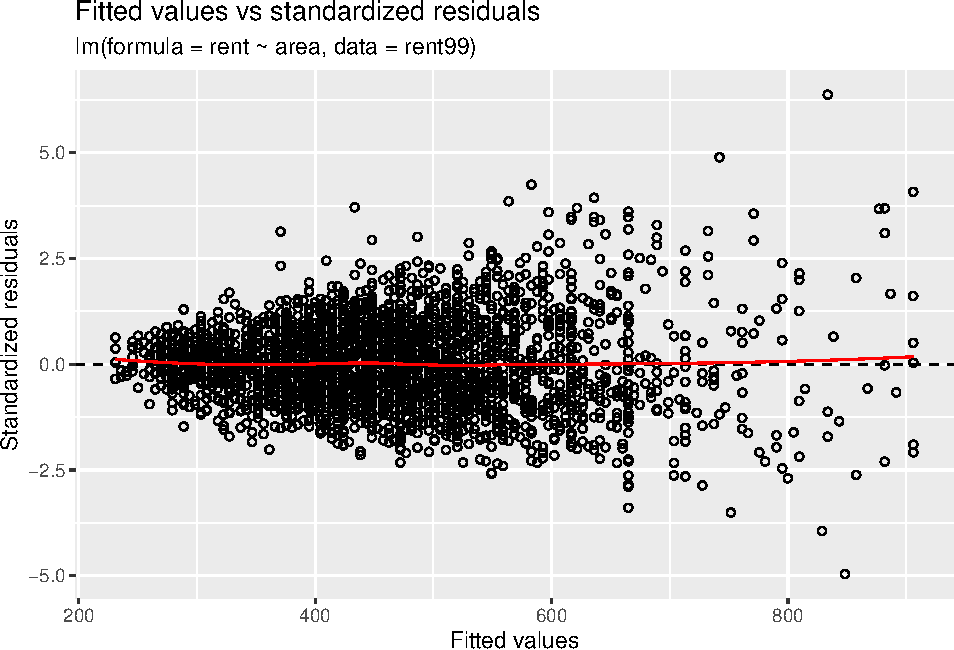
\includegraphics{2MLR_files/figure-latex/unnamed-chunk-9-1.pdf}

\begin{center}\rule{0.5\linewidth}{0.5pt}\end{center}

\hypertarget{normal-q-q}{%
\paragraph{Normal Q-Q}\label{normal-q-q}}

This plot shows if the residuals are Gaussian (normally) distributed. If
they follow a straigt line it is an indication that they are, and else
they are probably not.

\begin{center}\rule{0.5\linewidth}{0.5pt}\end{center}

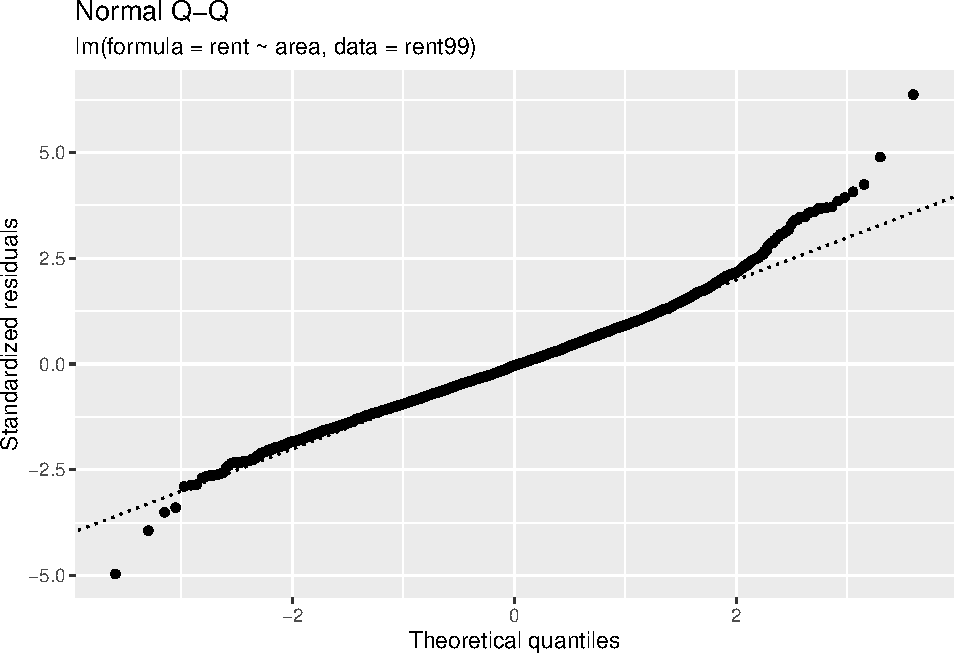
\includegraphics{2MLR_files/figure-latex/unnamed-chunk-10-1.pdf}

\begin{center}\rule{0.5\linewidth}{0.5pt}\end{center}

\begin{Shaded}
\begin{Highlighting}[]
\FunctionTok{library}\NormalTok{(nortest)}
\FunctionTok{ad.test}\NormalTok{(}\FunctionTok{rstudent}\NormalTok{(fit))}
\end{Highlighting}
\end{Shaded}

\begin{verbatim}
## 
##  Anderson-Darling normality test
## 
## data:  rstudent(fit)
## A = 6.4123, p-value = 9.809e-16
\end{verbatim}

\begin{center}\rule{0.5\linewidth}{0.5pt}\end{center}

\hypertarget{scale-location}{%
\paragraph{Scale-location}\label{scale-location}}

This is also called spread-location plot. It shows if the residuals are
spread equally along the ranges of predictors. Can be used to check the
assumption of equal variance (homoscedasticity). A good plot is one with
a horizontal line with randomly spread points.

Is this plot good for your data?

\begin{center}\rule{0.5\linewidth}{0.5pt}\end{center}

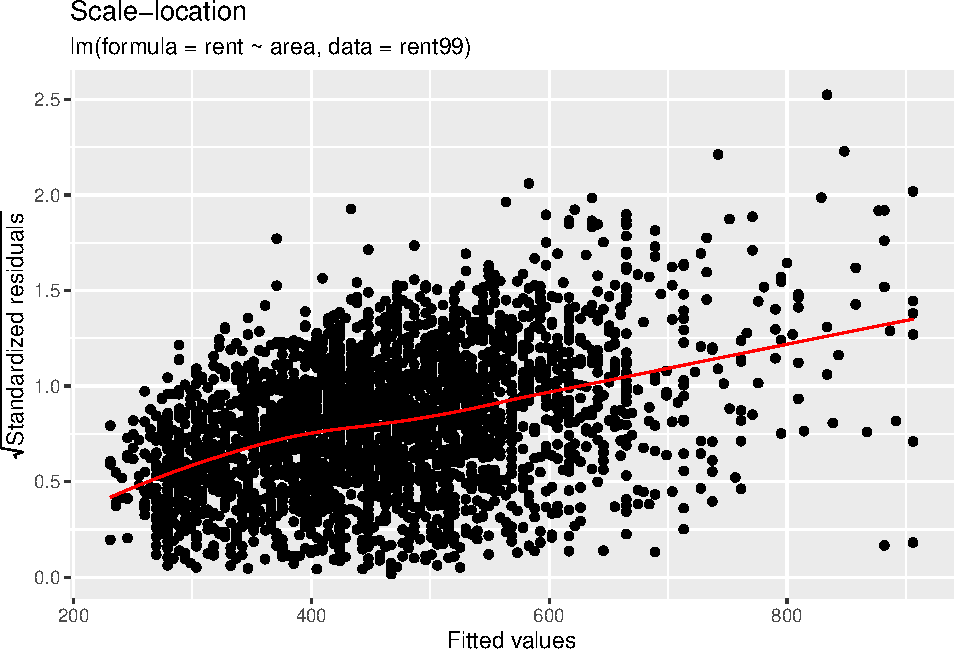
\includegraphics{2MLR_files/figure-latex/unnamed-chunk-12-1.pdf}

\begin{center}\rule{0.5\linewidth}{0.5pt}\end{center}

\hypertarget{residual-vs-leverage}{%
\paragraph{Residual vs Leverage}\label{residual-vs-leverage}}

This plot can reveal influential outliers. Not all outliers are
influential in linear regression; even though data have extreme values,
they might not be influential to determine the regression line (the
results don't differ much if they are removed from the data set). These
influential outliers can be seen as observations that does not get along
with the trend in the majority of the observations. In \texttt{plot.lm},
dashed lines are used to indicate the Cook's distance, instead of using
the size of the dots as is done here.

\begin{center}\rule{0.5\linewidth}{0.5pt}\end{center}

Cook's distance is the Euclidean distance between the
\(\mathbf{\hat{y}}\) (the fitted values) and \(\mathbf{\hat{y}}_{(i)}\)
(the fitted values calculated when the \(i\)-th observation is omitted
from the regression). This is then a measure on how much the model is
influences by observation \(i\). The distance is scaled, and a rule of
thumb is to examine observations with Cook's distance larger than 1, and
give some attention to those with Cook's distance above 0.5.

Leverage is defined as the diagonal elements of the hat matrix, i.e.,
the leverage of the \(i\)-th data point is \(h_{ii}\) on the diagonal of
\(\mathbf{H = X(X^TX)^{-1}X^T}\). A large leverage indicated that the
observation (\(i\)) has a large influence on the estimation results, and
that the covariate values (\(\mathbf{x}_i\)) are unusual.

\begin{center}\rule{0.5\linewidth}{0.5pt}\end{center}

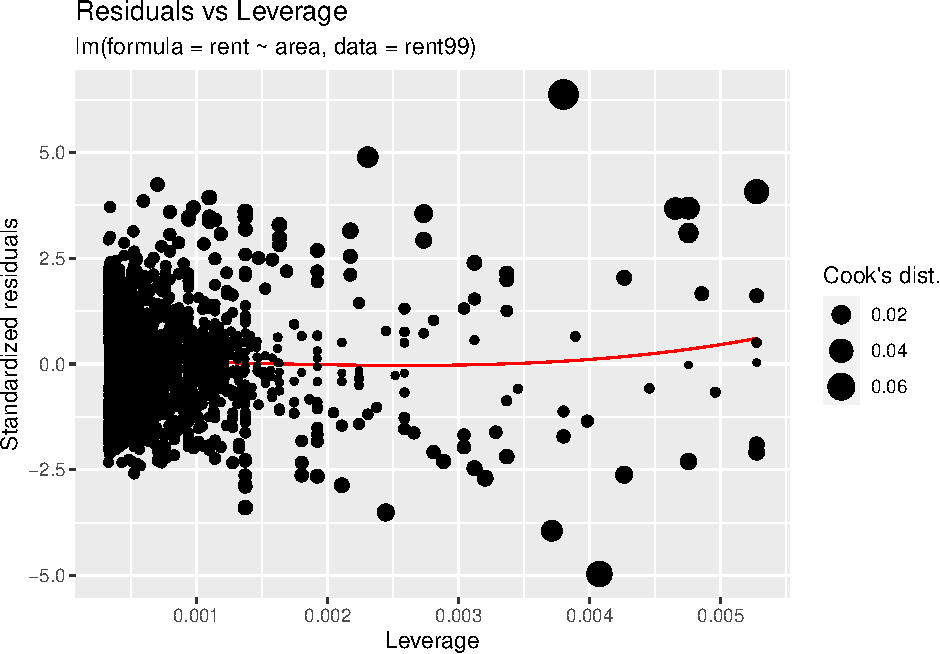
\includegraphics{2MLR_files/figure-latex/unnamed-chunk-13-1.pdf}

(Some observations does not fit our model, but if we fit a more complex
model this may change.)

\hypertarget{categorical-covariates---dummy-and-effect-coding}{%
\section{Categorical covariates - dummy and effect
coding}\label{categorical-covariates---dummy-and-effect-coding}}

(read for yourself - topic of ILw1)

\textbf{Example}: consider our \texttt{rent} dataset with \texttt{rent}
as reponse, and continuous covariate \texttt{area} and categorical
covariate \texttt{location}. Let the \texttt{location} be a factor with
levels \texttt{average,\ good,\ excellent}.

\begin{Shaded}
\begin{Highlighting}[]
\FunctionTok{library}\NormalTok{(gamlss.data)}
\FunctionTok{library}\NormalTok{(tidyverse)}
\FunctionTok{library}\NormalTok{(GGally)}
\end{Highlighting}
\end{Shaded}

\begin{Shaded}
\begin{Highlighting}[]
\NormalTok{ds }\OtherTok{=}\NormalTok{ rent99 }\SpecialCharTok{\%\textgreater{}\%}
    \FunctionTok{select}\NormalTok{(location, area, rent)}
\FunctionTok{levels}\NormalTok{(ds}\SpecialCharTok{$}\NormalTok{location)}
\end{Highlighting}
\end{Shaded}

\begin{verbatim}
## [1] "1" "2" "3"
\end{verbatim}

\begin{Shaded}
\begin{Highlighting}[]
\CommentTok{\# change to meaningful names}
\FunctionTok{levels}\NormalTok{(ds}\SpecialCharTok{$}\NormalTok{location) }\OtherTok{=} \FunctionTok{c}\NormalTok{(}\StringTok{"average"}\NormalTok{, }\StringTok{"good"}\NormalTok{, }\StringTok{"excellent"}\NormalTok{)}
\FunctionTok{ggpairs}\NormalTok{(ds)}
\end{Highlighting}
\end{Shaded}

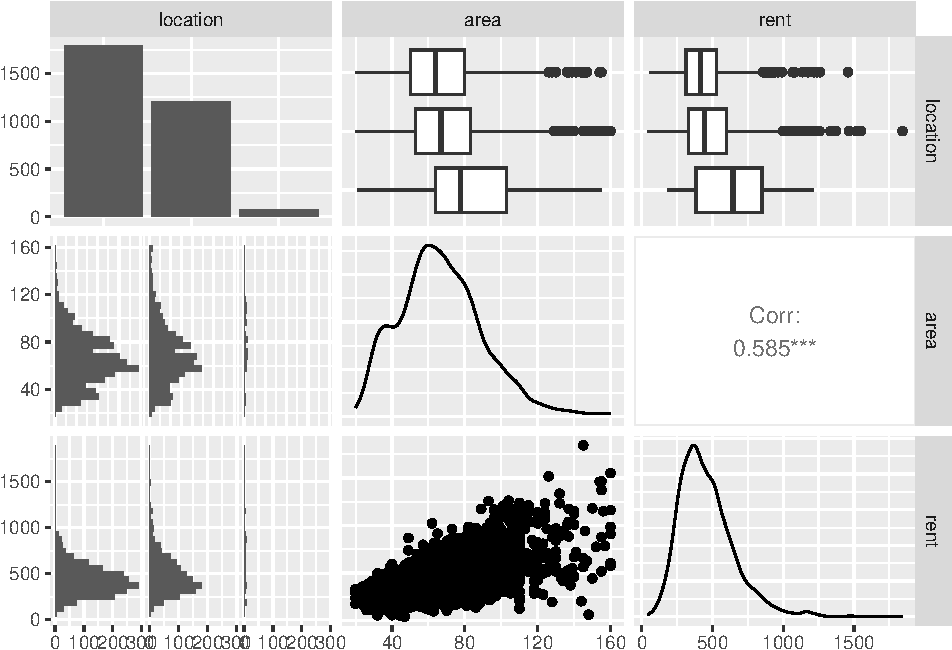
\includegraphics{2MLR_files/figure-latex/unnamed-chunk-15-1.pdf}

\textbf{Q}: comment on what you see in the \texttt{ggpairs} plot.

Categorical covariates may either be ordered or unordered. We will only
consider unordered categories here. In general, we could like to
estimate regression coefficients for all levels for the categorical
covariates. However, if we want to include an intercept in our model we
can only include codings for one less variable than the number of levels
we have - or else our design matrix will not have full rank.

\textbf{Q}: Assume you have a categorical variable with three levels.
Check for yourself that making a design matrix with one intercept and
three columns with dummy (0-1) variable coding will result in a matrix
that is singular.

\begin{Shaded}
\begin{Highlighting}[]
\CommentTok{\# make \textquotesingle{}wrong\textquotesingle{} dummy variable coding with 3 columns}
\NormalTok{n }\OtherTok{=} \FunctionTok{length}\NormalTok{(ds}\SpecialCharTok{$}\NormalTok{location)}
\NormalTok{X }\OtherTok{=} \FunctionTok{cbind}\NormalTok{(}\FunctionTok{rep}\NormalTok{(}\DecValTok{1}\NormalTok{, n), ds}\SpecialCharTok{$}\NormalTok{area, }\FunctionTok{rep}\NormalTok{(}\DecValTok{0}\NormalTok{, n), }\FunctionTok{rep}\NormalTok{(}\DecValTok{0}\NormalTok{, n), }\FunctionTok{rep}\NormalTok{(}\DecValTok{0}\NormalTok{, n))}
\NormalTok{X[ds}\SpecialCharTok{$}\NormalTok{location }\SpecialCharTok{==} \StringTok{"average"}\NormalTok{, }\DecValTok{3}\NormalTok{] }\OtherTok{=} \DecValTok{1}
\NormalTok{X[ds}\SpecialCharTok{$}\NormalTok{location }\SpecialCharTok{==} \StringTok{"good"}\NormalTok{, }\DecValTok{4}\NormalTok{] }\OtherTok{=} \DecValTok{1}
\NormalTok{X[ds}\SpecialCharTok{$}\NormalTok{location }\SpecialCharTok{==} \StringTok{"excellent"}\NormalTok{, }\DecValTok{5}\NormalTok{] }\OtherTok{=} \DecValTok{1}
\NormalTok{X[}\FunctionTok{c}\NormalTok{(}\DecValTok{1}\NormalTok{, }\DecValTok{3}\NormalTok{, }\DecValTok{69}\NormalTok{), ]}
\end{Highlighting}
\end{Shaded}

\begin{verbatim}
##      [,1] [,2] [,3] [,4] [,5]
## [1,]    1   26    0    1    0
## [2,]    1   30    1    0    0
## [3,]    1   55    0    0    1
\end{verbatim}

\begin{Shaded}
\begin{Highlighting}[]
\FunctionTok{library}\NormalTok{(Matrix)}
\FunctionTok{dim}\NormalTok{(X)}
\end{Highlighting}
\end{Shaded}

\begin{verbatim}
## [1] 3082    5
\end{verbatim}

\begin{Shaded}
\begin{Highlighting}[]
\FunctionTok{rankMatrix}\NormalTok{(X)}
\end{Highlighting}
\end{Shaded}

\begin{verbatim}
## [1] 4
## attr(,"method")
## [1] "tolNorm2"
## attr(,"useGrad")
## [1] FALSE
## attr(,"tol")
## [1] 6.843415e-13
\end{verbatim}

This is why we need to instead work with different ways of coding
categorical variables. One solution is to not include an intercept in
the model, but that is often not what we want. We will look at two other
solutions - one where we decide on a reference category (that we not
include in the coding, and therefore is kind of included in the
intercept - this is called ``treatment coding'') and one where we
require that the the sum of the coeffisients are zero (called ``effect
coding). This mainly effects how we interpret parameter estimates and
communicate our findings to the world.

If we fit a regression model with \texttt{lm} to the data with
\texttt{rent} as response and \texttt{area} and \texttt{location} as
covariates, a model matrix is made - and how to handle the categorical
variable is either specified the call to \texttt{lm} in
\texttt{contrasts=list(location="contr.treatment")} (or to model.matrix)
or globally for all categorical variables with
\texttt{options(contrasts=c("contr.treatment","contr.poly"))}- where
first element give choice for unordered factor (then treatment contrast
is default) and second for ordered (and then this polynomial contrast is
default). We will only work with unordered factors now.

--

\hypertarget{dummy-variable-coding-aka-treatment-contrast}{%
\subsubsection{Dummy variable coding aka treatment
contrast}\label{dummy-variable-coding-aka-treatment-contrast}}

This is the default coding. The reference level is automatically chosen
as the ``lowest'' level (sorted alphabetically). For our example this
means that the reference category for location is ``average''. If we
instead wanted ``good'' to be reference category we could relevel the
factor.

\begin{Shaded}
\begin{Highlighting}[]
\NormalTok{X1 }\OtherTok{=} \FunctionTok{model.matrix}\NormalTok{(}\SpecialCharTok{\textasciitilde{}}\NormalTok{area }\SpecialCharTok{+}\NormalTok{ location, }\AttributeTok{data =}\NormalTok{ ds)}
\NormalTok{X1[}\FunctionTok{c}\NormalTok{(}\DecValTok{1}\NormalTok{, }\DecValTok{3}\NormalTok{, }\DecValTok{69}\NormalTok{), ]}
\end{Highlighting}
\end{Shaded}

\begin{verbatim}
##    (Intercept) area locationgood locationexcellent
## 1            1   26            1                 0
## 3            1   30            0                 0
## 69           1   55            0                 1
\end{verbatim}

\begin{Shaded}
\begin{Highlighting}[]
\NormalTok{ds}\SpecialCharTok{$}\NormalTok{locationRELEVEL }\OtherTok{=} \FunctionTok{relevel}\NormalTok{(ds}\SpecialCharTok{$}\NormalTok{location, }\AttributeTok{ref =} \StringTok{"good"}\NormalTok{)}
\NormalTok{X2 }\OtherTok{=} \FunctionTok{model.matrix}\NormalTok{(}\SpecialCharTok{\textasciitilde{}}\NormalTok{area }\SpecialCharTok{+}\NormalTok{ locationRELEVEL, }\AttributeTok{data =}\NormalTok{ ds)}
\NormalTok{X2[}\FunctionTok{c}\NormalTok{(}\DecValTok{1}\NormalTok{, }\DecValTok{3}\NormalTok{, }\DecValTok{69}\NormalTok{), ]}
\end{Highlighting}
\end{Shaded}

\begin{verbatim}
##    (Intercept) area locationRELEVELaverage locationRELEVELexcellent
## 1            1   26                      0                        0
## 3            1   30                      1                        0
## 69           1   55                      0                        1
\end{verbatim}

So, what does this mean in practice? Model 1 has \texttt{average} as
reference category and model 2 \texttt{good}.

\begin{Shaded}
\begin{Highlighting}[]
\NormalTok{fit1 }\OtherTok{=} \FunctionTok{lm}\NormalTok{(rent }\SpecialCharTok{\textasciitilde{}}\NormalTok{ area }\SpecialCharTok{+}\NormalTok{ location, }\AttributeTok{data =}\NormalTok{ ds, }\AttributeTok{contrasts =} \FunctionTok{list}\NormalTok{(}\AttributeTok{location =} \StringTok{"contr.treatment"}\NormalTok{))}
\FunctionTok{summary}\NormalTok{(fit1)}
\end{Highlighting}
\end{Shaded}

\begin{verbatim}
## 
## Call:
## lm(formula = rent ~ area + location, data = ds, contrasts = list(location = "contr.treatment"))
## 
## Residuals:
##     Min      1Q  Median      3Q     Max 
## -790.98 -100.89   -4.87   94.47 1004.98 
## 
## Coefficients:
##                   Estimate Std. Error t value Pr(>|t|)    
## (Intercept)       128.0867     8.6947  14.732  < 2e-16 ***
## area                4.7056     0.1202  39.142  < 2e-16 ***
## locationgood       28.0040     5.8662   4.774 1.89e-06 ***
## locationexcellent 131.1075    18.2614   7.180 8.73e-13 ***
## ---
## Signif. codes:  0 '***' 0.001 '**' 0.01 '*' 0.05 '.' 0.1 ' ' 1
## 
## Residual standard error: 157.1 on 3078 degrees of freedom
## Multiple R-squared:  0.3555, Adjusted R-squared:  0.3549 
## F-statistic:   566 on 3 and 3078 DF,  p-value: < 2.2e-16
\end{verbatim}

\begin{Shaded}
\begin{Highlighting}[]
\NormalTok{fit2 }\OtherTok{=} \FunctionTok{lm}\NormalTok{(rent }\SpecialCharTok{\textasciitilde{}}\NormalTok{ area }\SpecialCharTok{+}\NormalTok{ locationRELEVEL, }\AttributeTok{data =}\NormalTok{ ds, }\AttributeTok{contrasts =} \FunctionTok{list}\NormalTok{(}\AttributeTok{locationRELEVEL =} \StringTok{"contr.treatment"}\NormalTok{))}
\FunctionTok{summary}\NormalTok{(fit2)}
\end{Highlighting}
\end{Shaded}

\begin{verbatim}
## 
## Call:
## lm(formula = rent ~ area + locationRELEVEL, data = ds, contrasts = list(locationRELEVEL = "contr.treatment"))
## 
## Residuals:
##     Min      1Q  Median      3Q     Max 
## -790.98 -100.89   -4.87   94.47 1004.98 
## 
## Coefficients:
##                          Estimate Std. Error t value Pr(>|t|)    
## (Intercept)              156.0907     9.4950  16.439  < 2e-16 ***
## area                       4.7056     0.1202  39.142  < 2e-16 ***
## locationRELEVELaverage   -28.0040     5.8662  -4.774 1.89e-06 ***
## locationRELEVELexcellent 103.1034    18.4021   5.603 2.30e-08 ***
## ---
## Signif. codes:  0 '***' 0.001 '**' 0.01 '*' 0.05 '.' 0.1 ' ' 1
## 
## Residual standard error: 157.1 on 3078 degrees of freedom
## Multiple R-squared:  0.3555, Adjusted R-squared:  0.3549 
## F-statistic:   566 on 3 and 3078 DF,  p-value: < 2.2e-16
\end{verbatim}

\textbf{Q}: Comment on the print-out. How do we interpret the intercept
estimate?

\begin{center}\rule{0.5\linewidth}{0.5pt}\end{center}

\hypertarget{effect-coding-aka-sum-zero-contrast}{%
\subsubsection{Effect coding aka
sum-zero-contrast:}\label{effect-coding-aka-sum-zero-contrast}}

This is an equally useful and popular coding - and this is the coding
that is preferred when working with analysis of variance in general. The
effect coding assumes that the sum of the effects for the levels of the
factor sums to zero, and this is done with the following coding scheme
(Model 3 with the original location and 4 with the releveled version.)

\begin{Shaded}
\begin{Highlighting}[]
\NormalTok{X3 }\OtherTok{=} \FunctionTok{model.matrix}\NormalTok{(}\SpecialCharTok{\textasciitilde{}}\NormalTok{area }\SpecialCharTok{+}\NormalTok{ location, }\AttributeTok{data =}\NormalTok{ ds, }\AttributeTok{contrasts =} \FunctionTok{list}\NormalTok{(}\AttributeTok{location =} \StringTok{"contr.sum"}\NormalTok{))}
\NormalTok{X3[}\FunctionTok{c}\NormalTok{(}\DecValTok{1}\NormalTok{, }\DecValTok{3}\NormalTok{, }\DecValTok{69}\NormalTok{), ]}
\end{Highlighting}
\end{Shaded}

\begin{verbatim}
##    (Intercept) area location1 location2
## 1            1   26         0         1
## 3            1   30         1         0
## 69           1   55        -1        -1
\end{verbatim}

\begin{Shaded}
\begin{Highlighting}[]
\NormalTok{X4 }\OtherTok{=} \FunctionTok{model.matrix}\NormalTok{(}\SpecialCharTok{\textasciitilde{}}\NormalTok{area }\SpecialCharTok{+}\NormalTok{ locationRELEVEL, }\AttributeTok{data =}\NormalTok{ ds, }\AttributeTok{contrasts =} \FunctionTok{list}\NormalTok{(}\AttributeTok{locationRELEVEL =} \StringTok{"contr.sum"}\NormalTok{))}
\NormalTok{X4[}\FunctionTok{c}\NormalTok{(}\DecValTok{1}\NormalTok{, }\DecValTok{3}\NormalTok{, }\DecValTok{69}\NormalTok{), ]}
\end{Highlighting}
\end{Shaded}

\begin{verbatim}
##    (Intercept) area locationRELEVEL1 locationRELEVEL2
## 1            1   26                1                0
## 3            1   30                0                1
## 69           1   55               -1               -1
\end{verbatim}

Observe the coding scheme. This means that when we find ``the missing
location level estimate'' as the negative of the sum of the parameter
estimates for the other estimated levels.

So, what does this mean in practice?

\begin{Shaded}
\begin{Highlighting}[]
\NormalTok{fit3 }\OtherTok{=} \FunctionTok{lm}\NormalTok{(rent }\SpecialCharTok{\textasciitilde{}}\NormalTok{ area }\SpecialCharTok{+}\NormalTok{ location, }\AttributeTok{data =}\NormalTok{ ds, }\AttributeTok{contrasts =} \FunctionTok{list}\NormalTok{(}\AttributeTok{location =} \StringTok{"contr.sum"}\NormalTok{))}
\FunctionTok{summary}\NormalTok{(fit3)}
\end{Highlighting}
\end{Shaded}

\begin{verbatim}
## 
## Call:
## lm(formula = rent ~ area + location, data = ds, contrasts = list(location = "contr.sum"))
## 
## Residuals:
##     Min      1Q  Median      3Q     Max 
## -790.98 -100.89   -4.87   94.47 1004.98 
## 
## Coefficients:
##             Estimate Std. Error t value Pr(>|t|)    
## (Intercept) 181.1238    10.6383  17.026  < 2e-16 ***
## area          4.7056     0.1202  39.142  < 2e-16 ***
## location1   -53.0372     6.6428  -7.984 1.98e-15 ***
## location2   -25.0331     6.7710  -3.697 0.000222 ***
## ---
## Signif. codes:  0 '***' 0.001 '**' 0.01 '*' 0.05 '.' 0.1 ' ' 1
## 
## Residual standard error: 157.1 on 3078 degrees of freedom
## Multiple R-squared:  0.3555, Adjusted R-squared:  0.3549 
## F-statistic:   566 on 3 and 3078 DF,  p-value: < 2.2e-16
\end{verbatim}

\begin{Shaded}
\begin{Highlighting}[]
\NormalTok{fit4 }\OtherTok{=} \FunctionTok{lm}\NormalTok{(rent }\SpecialCharTok{\textasciitilde{}}\NormalTok{ area }\SpecialCharTok{+}\NormalTok{ locationRELEVEL, }\AttributeTok{data =}\NormalTok{ ds, }\AttributeTok{contrasts =} \FunctionTok{list}\NormalTok{(}\AttributeTok{locationRELEVEL =} \StringTok{"contr.sum"}\NormalTok{))}
\FunctionTok{summary}\NormalTok{(fit4)}
\end{Highlighting}
\end{Shaded}

\begin{verbatim}
## 
## Call:
## lm(formula = rent ~ area + locationRELEVEL, data = ds, contrasts = list(locationRELEVEL = "contr.sum"))
## 
## Residuals:
##     Min      1Q  Median      3Q     Max 
## -790.98 -100.89   -4.87   94.47 1004.98 
## 
## Coefficients:
##                  Estimate Std. Error t value Pr(>|t|)    
## (Intercept)      181.1238    10.6383  17.026  < 2e-16 ***
## area               4.7056     0.1202  39.142  < 2e-16 ***
## locationRELEVEL1 -25.0331     6.7710  -3.697 0.000222 ***
## locationRELEVEL2 -53.0372     6.6428  -7.984 1.98e-15 ***
## ---
## Signif. codes:  0 '***' 0.001 '**' 0.01 '*' 0.05 '.' 0.1 ' ' 1
## 
## Residual standard error: 157.1 on 3078 degrees of freedom
## Multiple R-squared:  0.3555, Adjusted R-squared:  0.3549 
## F-statistic:   566 on 3 and 3078 DF,  p-value: < 2.2e-16
\end{verbatim}

\textbf{Q}: Comment on the print-out. How do we now interpret the
intercept estimate?

\hypertarget{interactions}{%
\section{Interactions}\label{interactions}}

(read for yourself)

To illustrate how interactions between covariates can be included we use
the \texttt{ozone} data set from the \texttt{ElemStatLearn} library.
This data set is measurements from 1973 in New York and contains 111
observations of the following variables:

\begin{itemize}
\tightlist
\item
  \texttt{ozone} : ozone concentration (ppm)
\item
  \texttt{radiation} : solar radiation (langleys)
\item
  \texttt{temperature} : daily maximum temperature (F)
\item
  \texttt{wind} : wind speed (mph)
\end{itemize}

\begin{center}\rule{0.5\linewidth}{0.5pt}\end{center}

We start by fitting a multiple linear regression model to the data, with
\texttt{ozone} as our response variable and \texttt{temperature} and
\texttt{wind} as covariates.

\begin{tabular}{r|r|r|r}
\hline
ozone & radiation & temperature & wind\\
\hline
41 & 190 & 67 & 7.4\\
\hline
36 & 118 & 72 & 8.0\\
\hline
12 & 149 & 74 & 12.6\\
\hline
18 & 313 & 62 & 11.5\\
\hline
23 & 299 & 65 & 8.6\\
\hline
19 & 99 & 59 & 13.8\\
\hline
\end{tabular}

\small

\begin{verbatim}
## 
## Call:
## lm(formula = ozone ~ temperature + wind, data = ozone)
## 
## Residuals:
##     Min      1Q  Median      3Q     Max 
## -42.160 -13.209  -3.089  10.588  98.470 
## 
## Coefficients:
##             Estimate Std. Error t value Pr(>|t|)    
## (Intercept) -67.2008    23.6083  -2.846  0.00529 ** 
## temperature   1.8265     0.2504   7.293 5.32e-11 ***
## wind         -3.2993     0.6706  -4.920 3.12e-06 ***
## ---
## Signif. codes:  0 '***' 0.001 '**' 0.01 '*' 0.05 '.' 0.1 ' ' 1
## 
## Residual standard error: 21.72 on 108 degrees of freedom
## Multiple R-squared:  0.5817, Adjusted R-squared:  0.574 
## F-statistic:  75.1 on 2 and 108 DF,  p-value: < 2.2e-16
\end{verbatim}

\normalsize

The model can be written as:
\[Y = \beta_0 + \beta_1 x_t + \beta_2 x_w + \varepsilon\] In this model
we have assumed that increasing the value of one covariate is
independent of the other covariates. For example: by increasing the
\texttt{temperature} by one-unit always increases the response value by
\(\beta_2 \approx 1.651\), regardless of the value of \texttt{wind}.

However, one might think that the covariate \texttt{wind} (wind speed)
might act differently upon \texttt{ozone} for different values of
\texttt{temperature} and vice verse.
\[\begin{aligned} Y &= \beta_0 +  \beta_1 x_t + \beta_2 x_w + \beta_3\cdot(x_t  \cdot x_w) +\varepsilon \\ &= \beta_0 +  (\beta_1 + \beta_3 x_w) \cdot x_t + \beta_2 x_w + \varepsilon \\ &= \beta_0 + \beta_1 x_t + (\beta_2 + \beta_3 x_t) \cdot x_w + \varepsilon \end{aligned}.\]
We fit this model in \texttt{R}. An interaction term can be included in
the model using the \texttt{*} symbol.

\textbf{Q:} Look at the \texttt{summary} below. Is this a better model
than without the interaction term? It the term significant?

\footnotesize

\begin{Shaded}
\begin{Highlighting}[]
\NormalTok{ozone.int }\OtherTok{=} \FunctionTok{lm}\NormalTok{(ozone }\SpecialCharTok{\textasciitilde{}}\NormalTok{ temperature }\SpecialCharTok{+}\NormalTok{ wind }\SpecialCharTok{+}\NormalTok{ temperature }\SpecialCharTok{*}\NormalTok{ wind, }\AttributeTok{data =}\NormalTok{ ozone)}
\FunctionTok{summary}\NormalTok{(ozone.int)}
\end{Highlighting}
\end{Shaded}

\begin{verbatim}
## 
## Call:
## lm(formula = ozone ~ temperature + wind + temperature * wind, 
##     data = ozone)
## 
## Residuals:
##     Min      1Q  Median      3Q     Max 
## -40.929 -11.190  -3.037   8.209  97.440 
## 
## Coefficients:
##                    Estimate Std. Error t value Pr(>|t|)    
## (Intercept)      -239.94146   48.59004  -4.938 2.92e-06 ***
## temperature         4.00151    0.59311   6.747 8.02e-10 ***
## wind               13.60882    4.28070   3.179  0.00193 ** 
## temperature:wind   -0.21747    0.05446  -3.993  0.00012 ***
## ---
## Signif. codes:  0 '***' 0.001 '**' 0.01 '*' 0.05 '.' 0.1 ' ' 1
## 
## Residual standard error: 20.36 on 107 degrees of freedom
## Multiple R-squared:  0.636,  Adjusted R-squared:  0.6258 
## F-statistic: 62.31 on 3 and 107 DF,  p-value: < 2.2e-16
\end{verbatim}

\normalsize

Below we see that the interaction term is highly significant. The
\(p\)-value is very small, so that there is strong evidence that
\(\beta_3 \neq 0\). Furthermore, \(R^2_{\text{adj}}\) has increased,
indicating that more of the variability in the data has been explained
by the model (than without the interaction).

\emph{Interpretation of the interaction term:}

\begin{itemize}
\item
  If we now increase the \texttt{temperature} by \(10^{\circ}\) F, the
  increase in \texttt{wind} speed will be
  \[(\hat \beta_1+\hat \beta_3 \cdot x_w) \cdot 10 = (4.0 -0.22 \cdot x_w) \cdot 10 = 40-2.2 x_w \text{ units}.\]
\item
  If we increase the \texttt{wind} speed by 10 mph, the increase in
  \texttt{temperature} will be
  \[(\hat \beta_2 + \hat \beta_3 \cdot x_t) \cdot 10 = (14 -0.22 \cdot x_t) \cdot 10 = 140-2.2 x_t \text{ units}.\]
\end{itemize}

\textbf{The hierarchical principle}

It is possible that the interaction term is higly significant, but the
main effects are not.

In our \texttt{ozone.int} model above: the main effects are
\texttt{temperature} and \texttt{wind}. The hierarchical principle
states that if we include an interaction term in our model, the main
effects are also to be included, even if they are not significant. This
means that if the coefficients \(\hat \beta_1\) or \(\hat \beta_2\)
would be insignificant, while the coefficient \(\hat \beta_3\) is
significant, \(\hat \beta_1\) and \(\hat \beta_2\) should still be
included in the model.

There reasons for this is that a model with interaction terms, but
without the main effects is hard to interpret.

\hypertarget{interactions-between-qualitative-discrete-and-quantitative-continuous-covariates}{%
\subsubsection{Interactions between qualitative (discrete) and
quantitative (continuous)
covariates}\label{interactions-between-qualitative-discrete-and-quantitative-continuous-covariates}}

We create a new variable \texttt{temp.cat} which is a
\texttt{temperature} as a qualitative covariate with two levels and fit
the model:
\[\begin{aligned}y&=\beta_0 + \beta_1 x_w + \begin{cases} \beta_2 + \beta_3  x_w  &\text{ if temperature="low"}\\ 0 &\text{ if temperature = "high"}\end{cases} \\\\ &= \begin{cases} (\beta_0 + \beta_2) + (\beta_1 + \beta_3) \cdot x_w &\text{ if temperature="low"}\\ \beta_0 + \beta_1 x_w &\text{ if temperature="high""} \end{cases} \end{aligned}\]

\begin{tabular}{r|r|r|r|l}
\hline
ozone & radiation & temperature & wind & temp.cat\\
\hline
41 & 190 & 67 & 7.4 & low\\
\hline
36 & 118 & 72 & 8.0 & low\\
\hline
12 & 149 & 74 & 12.6 & low\\
\hline
18 & 313 & 62 & 11.5 & low\\
\hline
23 & 299 & 65 & 8.6 & low\\
\hline
19 & 99 & 59 & 13.8 & low\\
\hline
\end{tabular}

\begin{verbatim}
## 
## Call:
## lm(formula = ozone ~ wind + temp.cat + temp.cat * wind, data = ozone2)
## 
## Residuals:
##     Min      1Q  Median      3Q     Max 
## -53.291  -9.091  -1.307  11.227  71.815 
## 
## Coefficients:
##                  Estimate Std. Error t value Pr(>|t|)    
## (Intercept)      119.0450     7.5004  15.872  < 2e-16 ***
## wind              -6.7235     0.8195  -8.204 5.61e-13 ***
## temp.catlow      -92.6316    12.9466  -7.155 1.09e-10 ***
## wind:temp.catlow   6.0544     1.1999   5.046 1.86e-06 ***
## ---
## Signif. codes:  0 '***' 0.001 '**' 0.01 '*' 0.05 '.' 0.1 ' ' 1
## 
## Residual standard error: 20.26 on 107 degrees of freedom
## Multiple R-squared:  0.6393, Adjusted R-squared:  0.6291 
## F-statistic:  63.2 on 3 and 107 DF,  p-value: < 2.2e-16
\end{verbatim}

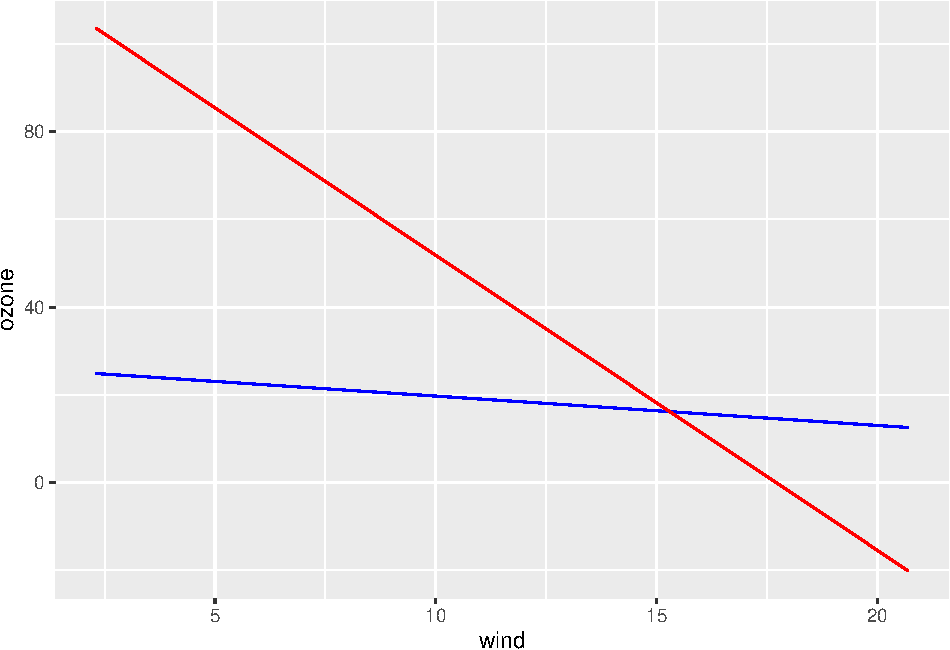
\includegraphics{2MLR_files/figure-latex/unnamed-chunk-25-1.pdf}

\begin{center}\rule{0.5\linewidth}{0.5pt}\end{center}

\hypertarget{interactive-lectures--problem-set-first-week}{%
\section{Interactive lectures- problem set first
week}\label{interactive-lectures--problem-set-first-week}}

\hypertarget{theoretical-questions}{%
\subsection{Theoretical questions}\label{theoretical-questions}}

\hypertarget{problem-1}{%
\subsubsection{Problem 1}\label{problem-1}}

\begin{enumerate}
\def\labelenumi{\arabic{enumi}.}
\item
  Write down the GLM way for the multiple linear regression model.
  Explain.
\item
  Write down the likelihood and loglikelihood. Then define the score
  vector. What is the set of equations we solve to find parameter
  estimates? What if we could not find a closed form solution to our set
  of equations - what could we do then?
\item
  Define the observed and the expected Fisher information matrix. What
  dimension does these matrices have? What can these matrices tell us?
\end{enumerate}

\begin{center}\rule{0.5\linewidth}{0.5pt}\end{center}

\begin{enumerate}
\def\labelenumi{\arabic{enumi}.}
\setcounter{enumi}{3}
\tightlist
\item
  A core finding is \(\hat \beta\).
  \[ \hat{\beta}=({\bf X}^T{\bf X})^{-1} {\bf X}^T {\bf Y}\] with
  \(\hat{\beta}\sim N_{p}(\beta,\sigma^2({\bf X}^T{\bf X})^{-1})\).
\end{enumerate}

Show that \(\hat{\beta}\) has this distribution with the given mean and
covariance matrix. What does this imply for the distribution of the
\(j\)th element of \(\hat{\beta}\)? In particular, how can we calculate
the variance of \(\hat{\beta}_j\)?

\begin{enumerate}
\def\labelenumi{\arabic{enumi}.}
\setcounter{enumi}{4}
\item
  Explain the difference between \emph{error} and \emph{residual}. What
  are the properties of the raw residuals? Why don't we want to use the
  raw residuals for model check? What is our solution to this?
\item
  That is the theoretical intercept and slope of a QQ--plot based on a
  normal sample? Hint:
  \href{https://www.math.ntnu.no/emner/TMA4315/2017h/qq.html}{QQ--plot
  as html}
\end{enumerate}

\begin{center}\rule{0.5\linewidth}{0.5pt}\end{center}

\hypertarget{interpretation-and-understanding}{%
\subsection{Interpretation and
understanding}\label{interpretation-and-understanding}}

\hypertarget{problem-2-munich-rent-index-data}{%
\subsubsection{Problem 2: Munich Rent Index
data}\label{problem-2-munich-rent-index-data}}

Fit the regression model with first \texttt{rent} and then
\texttt{rentsqm} as reponse and following covariates: \texttt{area},
\texttt{location} (dummy variable coding using location2 and location3),
\texttt{bath}, \texttt{kitchen} and \texttt{cheating} (central heating).

\begin{Shaded}
\begin{Highlighting}[]
\FunctionTok{library}\NormalTok{(gamlss.data)}
\FunctionTok{library}\NormalTok{(ggfortify)}
\StringTok{\textasciigrave{}}\AttributeTok{?}\StringTok{\textasciigrave{}}\NormalTok{(rent99)}

\NormalTok{mod1 }\OtherTok{\textless{}{-}} \FunctionTok{lm}\NormalTok{(rent }\SpecialCharTok{\textasciitilde{}}\NormalTok{ area }\SpecialCharTok{+}\NormalTok{ location }\SpecialCharTok{+}\NormalTok{ bath }\SpecialCharTok{+}\NormalTok{ kitchen }\SpecialCharTok{+}\NormalTok{ cheating, }\AttributeTok{data =}\NormalTok{ rent99)}
\NormalTok{mod2 }\OtherTok{\textless{}{-}} \FunctionTok{lm}\NormalTok{(rentsqm }\SpecialCharTok{\textasciitilde{}}\NormalTok{ area }\SpecialCharTok{+}\NormalTok{ location }\SpecialCharTok{+}\NormalTok{ bath }\SpecialCharTok{+}\NormalTok{ kitchen }\SpecialCharTok{+}\NormalTok{ cheating, }\AttributeTok{data =}\NormalTok{ rent99)}
\FunctionTok{autoplot}\NormalTok{(mod1, }\AttributeTok{label.size =} \DecValTok{2}\NormalTok{)}
\end{Highlighting}
\end{Shaded}

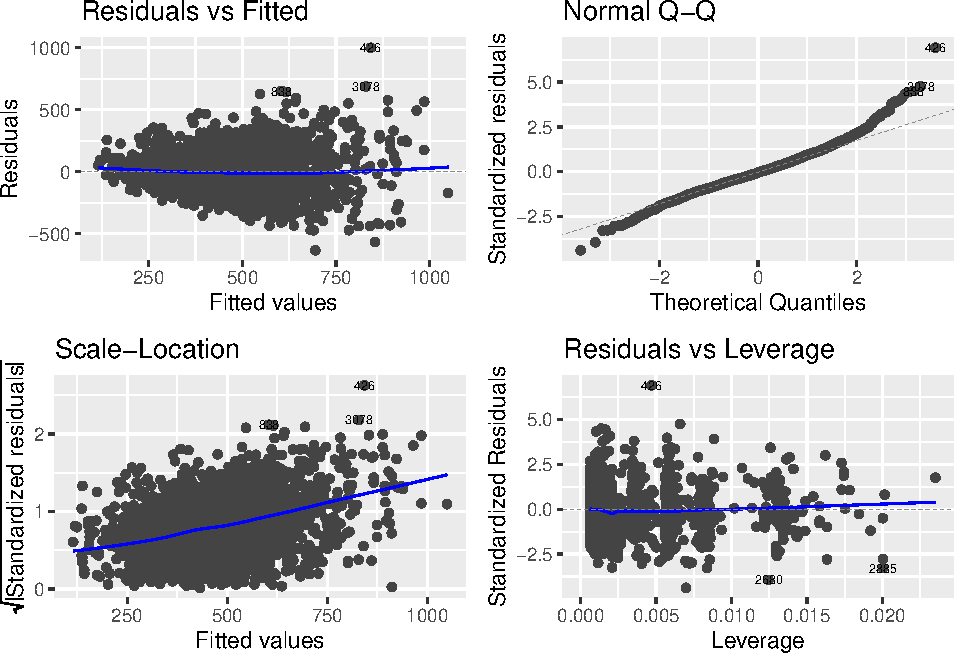
\includegraphics{2MLR_files/figure-latex/unnamed-chunk-26-1.pdf}

\begin{Shaded}
\begin{Highlighting}[]
\FunctionTok{autoplot}\NormalTok{(mod2, }\AttributeTok{label.size =} \DecValTok{2}\NormalTok{)}
\end{Highlighting}
\end{Shaded}

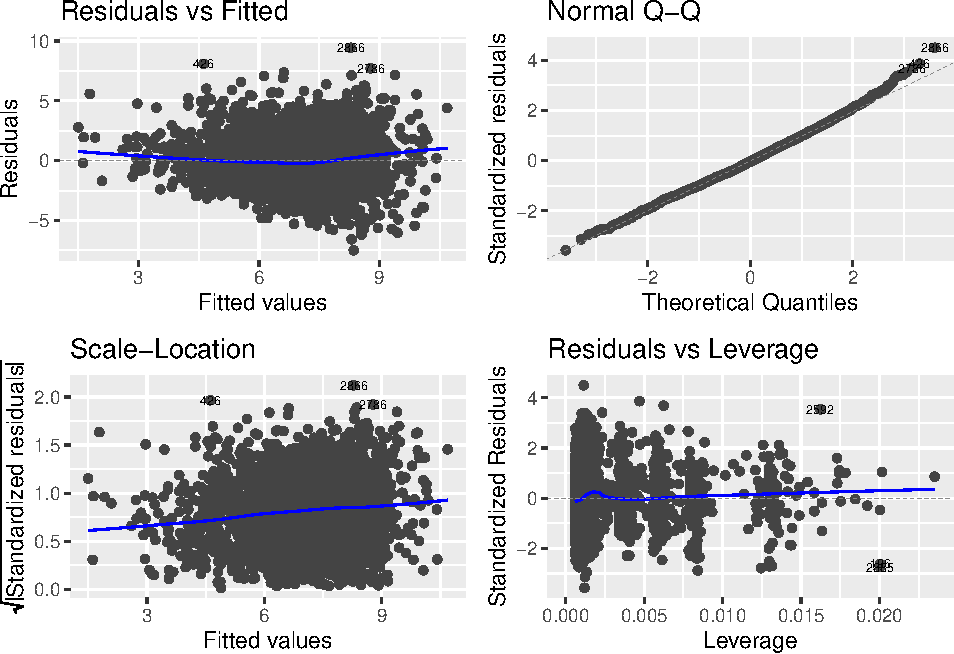
\includegraphics{2MLR_files/figure-latex/unnamed-chunk-26-2.pdf}

\begin{enumerate}
\def\labelenumi{\arabic{enumi}.}
\tightlist
\item
  Look at diagnostic plots for the two fits. Which response do you
  prefer?
\end{enumerate}

Consentrate on the response-model you choose for the rest of the tasks.

\begin{enumerate}
\def\labelenumi{\arabic{enumi}.}
\setcounter{enumi}{1}
\tightlist
\item
  Explain what the parameter estimates mean in practice. In particular,
  what is the interpretation of the intercept?
\end{enumerate}

\begin{Shaded}
\begin{Highlighting}[]
\FunctionTok{summary}\NormalTok{(mod1)}
\end{Highlighting}
\end{Shaded}

\begin{verbatim}
## 
## Call:
## lm(formula = rent ~ area + location + bath + kitchen + cheating, 
##     data = rent99)
## 
## Residuals:
##     Min      1Q  Median      3Q     Max 
## -633.41  -89.17   -6.26   82.96 1000.76 
## 
## Coefficients:
##             Estimate Std. Error t value Pr(>|t|)    
## (Intercept) -21.9733    11.6549  -1.885   0.0595 .  
## area          4.5788     0.1143  40.055  < 2e-16 ***
## location2    39.2602     5.4471   7.208 7.14e-13 ***
## location3   126.0575    16.8747   7.470 1.04e-13 ***
## bath1        74.0538    11.2087   6.607 4.61e-11 ***
## kitchen1    120.4349    13.0192   9.251  < 2e-16 ***
## cheating1   161.4138     8.6632  18.632  < 2e-16 ***
## ---
## Signif. codes:  0 '***' 0.001 '**' 0.01 '*' 0.05 '.' 0.1 ' ' 1
## 
## Residual standard error: 145.2 on 3075 degrees of freedom
## Multiple R-squared:  0.4504, Adjusted R-squared:  0.4494 
## F-statistic:   420 on 6 and 3075 DF,  p-value: < 2.2e-16
\end{verbatim}

\begin{Shaded}
\begin{Highlighting}[]
\FunctionTok{summary}\NormalTok{(mod2)}
\end{Highlighting}
\end{Shaded}

\begin{verbatim}
## 
## Call:
## lm(formula = rentsqm ~ area + location + bath + kitchen + cheating, 
##     data = rent99)
## 
## Residuals:
##     Min      1Q  Median      3Q     Max 
## -7.4959 -1.4084 -0.0733  1.3847  9.4400 
## 
## Coefficients:
##              Estimate Std. Error t value Pr(>|t|)    
## (Intercept)  7.108319   0.168567  42.169  < 2e-16 ***
## area        -0.038154   0.001653 -23.077  < 2e-16 ***
## location2    0.628698   0.078782   7.980 2.04e-15 ***
## location3    1.686099   0.244061   6.909 5.93e-12 ***
## bath1        0.989898   0.162113   6.106 1.15e-09 ***
## kitchen1     1.412113   0.188299   7.499 8.34e-14 ***
## cheating1    2.414101   0.125297  19.267  < 2e-16 ***
## ---
## Signif. codes:  0 '***' 0.001 '**' 0.01 '*' 0.05 '.' 0.1 ' ' 1
## 
## Residual standard error: 2.1 on 3075 degrees of freedom
## Multiple R-squared:  0.2584, Adjusted R-squared:  0.2569 
## F-statistic: 178.6 on 6 and 3075 DF,  p-value: < 2.2e-16
\end{verbatim}

\begin{enumerate}
\def\labelenumi{\arabic{enumi}.}
\setcounter{enumi}{2}
\tightlist
\item
  Go through the summary printout and explain the parts you know now,
  and also observe the parts you don't know yet (on the agenda for next
  week?).
\end{enumerate}

Next week: more on inference on this data set.

\begin{center}\rule{0.5\linewidth}{0.5pt}\end{center}

\hypertarget{problem-3-simple-vs.-multiple-regression}{%
\subsubsection{Problem 3: Simple vs.~multiple
regression}\label{problem-3-simple-vs.-multiple-regression}}

We look at a regression problem where both the response and the
covariates are centered - that is, the mean of the response and the mean
of each covariate is zero. We do this to avoid the intercept term, which
makes things a bit more complicated.

\begin{enumerate}
\def\labelenumi{\arabic{enumi}.}
\item
  In a design matrix (without an intercept column) orthogonal columns
  gives diagonal \({\bf X}^T {\bf X}\). What does that mean? How can we
  get orthogonal columns?
\item
  If we have orthogonal columns, will then simple (only one covariate)
  and multiple estimated regression coefficients be different? Explain.
\item
  What is multicollinearity? Is that a problem? Why (not)?
\end{enumerate}

\begin{center}\rule{0.5\linewidth}{0.5pt}\end{center}

\hypertarget{problem-4-dummy-vs.-effect-coding-in-mlr}{%
\subsubsection{Problem 4: Dummy vs.~effect coding in
MLR}\label{problem-4-dummy-vs.-effect-coding-in-mlr}}

Background material for this task: {[}Categorical covariates - dummy and
effect coding)(\#categorical)

We will study a dataset where we want to model \texttt{income} as
response and two unordered categorical covariates \texttt{gender}and
\texttt{place} (location).

\begin{Shaded}
\begin{Highlighting}[]
\NormalTok{income }\OtherTok{\textless{}{-}} \FunctionTok{c}\NormalTok{(}\DecValTok{300}\NormalTok{, }\DecValTok{350}\NormalTok{, }\DecValTok{370}\NormalTok{, }\DecValTok{360}\NormalTok{, }\DecValTok{400}\NormalTok{, }\DecValTok{370}\NormalTok{, }\DecValTok{420}\NormalTok{, }\DecValTok{390}\NormalTok{, }\DecValTok{400}\NormalTok{, }\DecValTok{430}\NormalTok{, }\DecValTok{420}\NormalTok{, }\DecValTok{410}\NormalTok{,}
    \DecValTok{300}\NormalTok{, }\DecValTok{320}\NormalTok{, }\DecValTok{310}\NormalTok{, }\DecValTok{305}\NormalTok{, }\DecValTok{350}\NormalTok{, }\DecValTok{370}\NormalTok{, }\DecValTok{340}\NormalTok{, }\DecValTok{355}\NormalTok{, }\DecValTok{370}\NormalTok{, }\DecValTok{380}\NormalTok{, }\DecValTok{360}\NormalTok{, }\DecValTok{365}\NormalTok{)}
\NormalTok{gender }\OtherTok{\textless{}{-}} \FunctionTok{c}\NormalTok{(}\FunctionTok{rep}\NormalTok{(}\StringTok{"Male"}\NormalTok{, }\DecValTok{12}\NormalTok{), }\FunctionTok{rep}\NormalTok{(}\StringTok{"Female"}\NormalTok{, }\DecValTok{12}\NormalTok{))}
\NormalTok{place }\OtherTok{\textless{}{-}} \FunctionTok{rep}\NormalTok{(}\FunctionTok{c}\NormalTok{(}\FunctionTok{rep}\NormalTok{(}\StringTok{"A"}\NormalTok{, }\DecValTok{4}\NormalTok{), }\FunctionTok{rep}\NormalTok{(}\StringTok{"B"}\NormalTok{, }\DecValTok{4}\NormalTok{), }\FunctionTok{rep}\NormalTok{(}\StringTok{"C"}\NormalTok{, }\DecValTok{4}\NormalTok{)), }\DecValTok{2}\NormalTok{)}
\NormalTok{data }\OtherTok{\textless{}{-}} \FunctionTok{data.frame}\NormalTok{(income, }\AttributeTok{gender =} \FunctionTok{factor}\NormalTok{(gender, }\AttributeTok{levels =} \FunctionTok{c}\NormalTok{(}\StringTok{"Female"}\NormalTok{,}
    \StringTok{"Male"}\NormalTok{)), }\AttributeTok{place =} \FunctionTok{factor}\NormalTok{(place, }\AttributeTok{levels =} \FunctionTok{c}\NormalTok{(}\StringTok{"A"}\NormalTok{, }\StringTok{"B"}\NormalTok{, }\StringTok{"C"}\NormalTok{)))}
\end{Highlighting}
\end{Shaded}

\begin{enumerate}
\def\labelenumi{\arabic{enumi}.}
\tightlist
\item
  First, describe the data set.
\end{enumerate}

\begin{Shaded}
\begin{Highlighting}[]
\FunctionTok{library}\NormalTok{(GGally)}
\NormalTok{GGally}\SpecialCharTok{::}\FunctionTok{ggpairs}\NormalTok{(data)}
\end{Highlighting}
\end{Shaded}

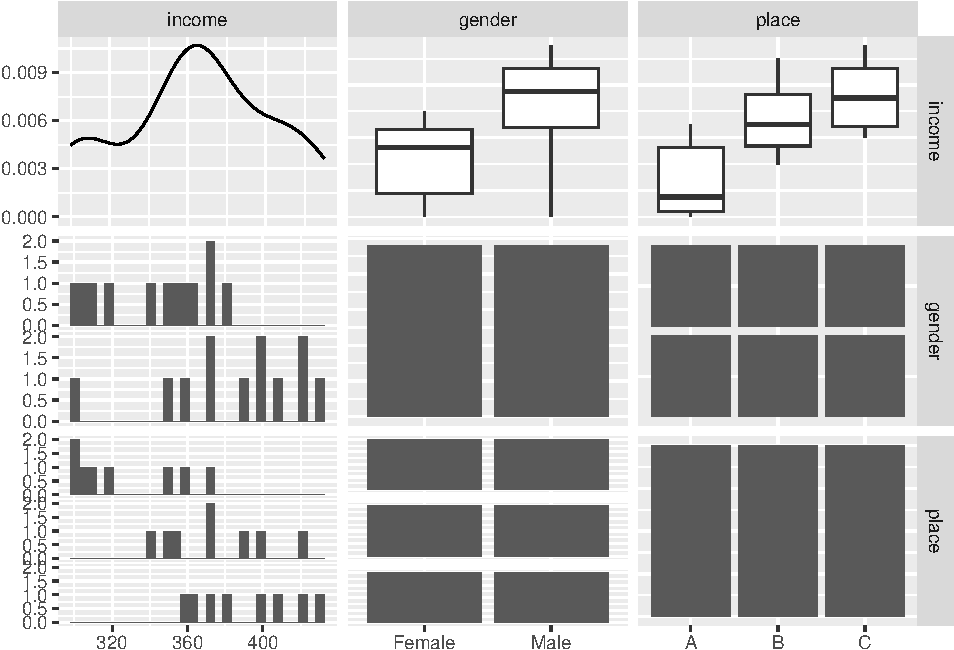
\includegraphics{2MLR_files/figure-latex/unnamed-chunk-29-1.pdf}

\begin{enumerate}
\def\labelenumi{\arabic{enumi}.}
\setcounter{enumi}{1}
\tightlist
\item
  Check out the
  \texttt{interaction.plot(data\$gender,data\$place,data\$income)}. What
  does it show? Do we need an interaction term if we want to model a MLR
  with \texttt{income} as response?
\end{enumerate}

\begin{Shaded}
\begin{Highlighting}[]
\FunctionTok{interaction.plot}\NormalTok{(}\AttributeTok{x.factor =}\NormalTok{ data}\SpecialCharTok{$}\NormalTok{gender, }\AttributeTok{trace.factor =}\NormalTok{ data}\SpecialCharTok{$}\NormalTok{place, }\AttributeTok{response =}\NormalTok{ data}\SpecialCharTok{$}\NormalTok{income,}
    \AttributeTok{type =} \StringTok{"l"}\NormalTok{)}
\end{Highlighting}
\end{Shaded}

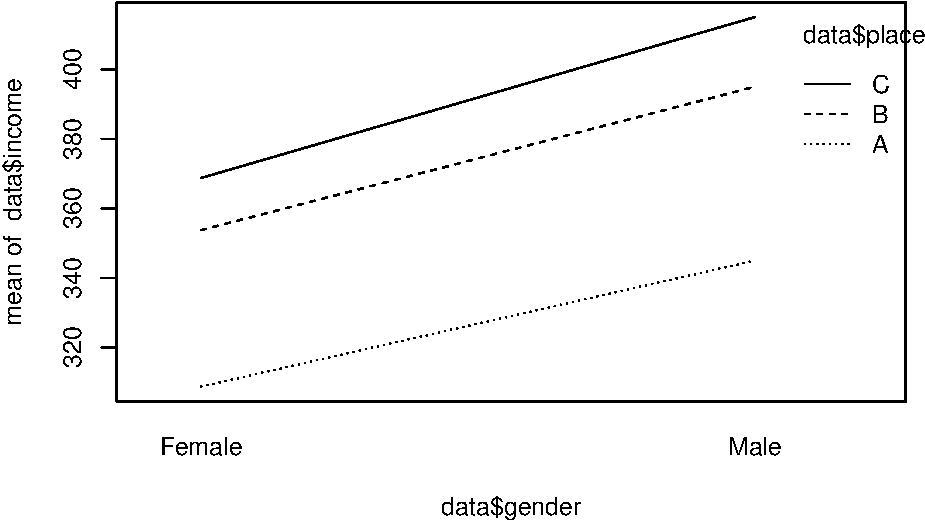
\includegraphics{2MLR_files/figure-latex/unnamed-chunk-30-1.pdf}

\begin{enumerate}
\def\labelenumi{\arabic{enumi}.}
\setcounter{enumi}{2}
\tightlist
\item
  Check our
  \texttt{plot.design(income\textasciitilde{}place+gender,\ data\ =\ data)}.
  What does it show?
\end{enumerate}

\begin{Shaded}
\begin{Highlighting}[]
\FunctionTok{plot.design}\NormalTok{(income }\SpecialCharTok{\textasciitilde{}}\NormalTok{ place }\SpecialCharTok{+}\NormalTok{ gender, }\AttributeTok{data =}\NormalTok{ data)}
\end{Highlighting}
\end{Shaded}

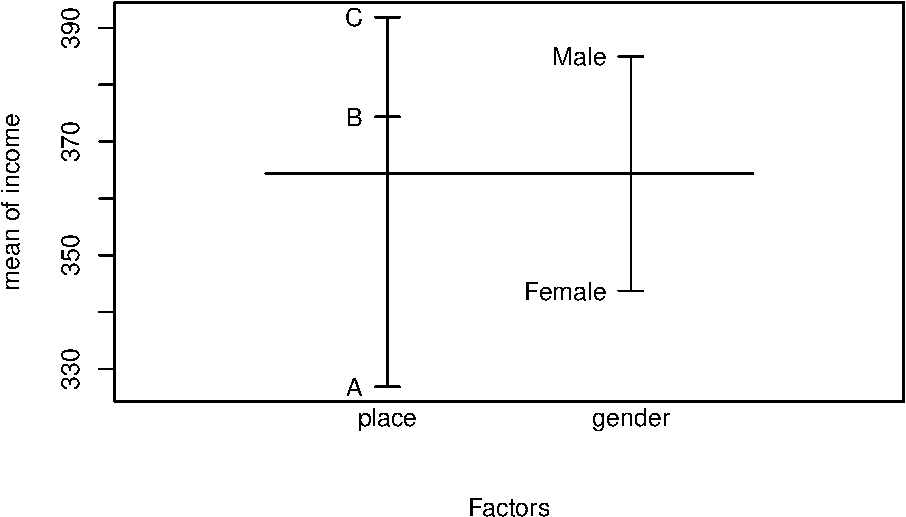
\includegraphics{2MLR_files/figure-latex/unnamed-chunk-31-1.pdf}

\begin{enumerate}
\def\labelenumi{\arabic{enumi}.}
\setcounter{enumi}{3}
\tightlist
\item
  First, use treatment contrast (dummy variable coding) and fit a MLR
  with \texttt{income} as response and \texttt{gender} and
  \texttt{place} as covariates. Explain what your model estimates mean.
  In particular, what is the interpretation of the intercept estimate?
\end{enumerate}

\begin{Shaded}
\begin{Highlighting}[]
\NormalTok{mod3 }\OtherTok{\textless{}{-}} \FunctionTok{lm}\NormalTok{(income }\SpecialCharTok{\textasciitilde{}}\NormalTok{ place }\SpecialCharTok{+}\NormalTok{ gender, }\AttributeTok{data =}\NormalTok{ data)}
\NormalTok{mod3}
\end{Highlighting}
\end{Shaded}

\begin{verbatim}
## 
## Call:
## lm(formula = income ~ place + gender, data = data)
## 
## Coefficients:
## (Intercept)       placeB       placeC   genderMale  
##      306.25        47.50        65.00        41.25
\end{verbatim}

\begin{enumerate}
\def\labelenumi{\arabic{enumi}.}
\setcounter{enumi}{4}
\tightlist
\item
  Now, turn to sum-zero contrast (effect coding). Explain what your
  model estimates mean. Now, what is the intercept estimate? Calculate
  the estimate for \texttt{place=C}.
\end{enumerate}

\begin{Shaded}
\begin{Highlighting}[]
\NormalTok{mod4 }\OtherTok{\textless{}{-}} \FunctionTok{lm}\NormalTok{(income }\SpecialCharTok{\textasciitilde{}}\NormalTok{ place }\SpecialCharTok{+}\NormalTok{ gender, }\AttributeTok{data =}\NormalTok{ data, }\AttributeTok{contrasts =} \FunctionTok{list}\NormalTok{(}\AttributeTok{place =} \StringTok{"contr.sum"}\NormalTok{,}
    \AttributeTok{gender =} \StringTok{"contr.sum"}\NormalTok{))}
\NormalTok{mod4}
\end{Highlighting}
\end{Shaded}

\begin{verbatim}
## 
## Call:
## lm(formula = income ~ place + gender, data = data, contrasts = list(place = "contr.sum", 
##     gender = "contr.sum"))
## 
## Coefficients:
## (Intercept)       place1       place2      gender1  
##      364.38       -37.50        10.00       -20.62
\end{verbatim}

\begin{Shaded}
\begin{Highlighting}[]
\FunctionTok{model.matrix}\NormalTok{(mod4)}
\end{Highlighting}
\end{Shaded}

\begin{verbatim}
##    (Intercept) place1 place2 gender1
## 1            1      1      0      -1
## 2            1      1      0      -1
## 3            1      1      0      -1
## 4            1      1      0      -1
## 5            1      0      1      -1
## 6            1      0      1      -1
## 7            1      0      1      -1
## 8            1      0      1      -1
## 9            1     -1     -1      -1
## 10           1     -1     -1      -1
## 11           1     -1     -1      -1
## 12           1     -1     -1      -1
## 13           1      1      0       1
## 14           1      1      0       1
## 15           1      1      0       1
## 16           1      1      0       1
## 17           1      0      1       1
## 18           1      0      1       1
## 19           1      0      1       1
## 20           1      0      1       1
## 21           1     -1     -1       1
## 22           1     -1     -1       1
## 23           1     -1     -1       1
## 24           1     -1     -1       1
## attr(,"assign")
## [1] 0 1 1 2
## attr(,"contrasts")
## attr(,"contrasts")$place
## [1] "contr.sum"
## 
## attr(,"contrasts")$gender
## [1] "contr.sum"
\end{verbatim}

\begin{Shaded}
\begin{Highlighting}[]
\FunctionTok{mean}\NormalTok{(income)}
\end{Highlighting}
\end{Shaded}

\begin{verbatim}
## [1] 364.375
\end{verbatim}

Next week we connect this to linear hypotheses and ANOVA.

\begin{center}\rule{0.5\linewidth}{0.5pt}\end{center}

\hypertarget{problem-5-interactions}{%
\subsubsection{Problem 5: Interactions}\label{problem-5-interactions}}

This part of the module was marked ``self-study''. Go through this
together in the group, and make sure that you understand.

\hypertarget{problem-6-simulations-in-r-optional}{%
\subsubsection{Problem 6: Simulations in R
(optional)}\label{problem-6-simulations-in-r-optional}}

(a version this problem was also given as recommended exercise in
TMA4268 Statistical learning)

\begin{enumerate}
\def\labelenumi{\arabic{enumi}.}
\tightlist
\item
  For simple linear regression, simulate at data set with homoscedastic
  errore and with heteroscedastic errors. Here is a suggestion of one
  solution. Why this? To see how things looks when the model is correct
  and wrong. Look at the code and discuss what is done, and relate this
  to the plots of errors (which are usually unobserved) and plots of
  residuals.
\end{enumerate}

\begin{Shaded}
\begin{Highlighting}[]
\CommentTok{\# Homoscedastic errors}
\NormalTok{n }\OtherTok{=} \DecValTok{1000}
\NormalTok{x }\OtherTok{=} \FunctionTok{seq}\NormalTok{(}\SpecialCharTok{{-}}\DecValTok{3}\NormalTok{, }\DecValTok{3}\NormalTok{, }\AttributeTok{length =}\NormalTok{ n)}
\NormalTok{beta0 }\OtherTok{=} \SpecialCharTok{{-}}\DecValTok{1}
\NormalTok{beta1 }\OtherTok{=} \DecValTok{2}
\NormalTok{xbeta }\OtherTok{=}\NormalTok{ beta0 }\SpecialCharTok{+}\NormalTok{ beta1 }\SpecialCharTok{*}\NormalTok{ x}
\NormalTok{sigma }\OtherTok{=} \DecValTok{1}
\NormalTok{e1 }\OtherTok{=} \FunctionTok{rnorm}\NormalTok{(n, }\AttributeTok{mean =} \DecValTok{0}\NormalTok{, }\AttributeTok{sd =}\NormalTok{ sigma)}
\NormalTok{y1 }\OtherTok{=}\NormalTok{ xbeta }\SpecialCharTok{+}\NormalTok{ e1}
\NormalTok{ehat1 }\OtherTok{=} \FunctionTok{residuals}\NormalTok{(}\FunctionTok{lm}\NormalTok{(y1 }\SpecialCharTok{\textasciitilde{}}\NormalTok{ x))}
\FunctionTok{plot}\NormalTok{(x, y1, }\AttributeTok{pch =} \DecValTok{20}\NormalTok{)}
\FunctionTok{abline}\NormalTok{(beta0, beta1, }\AttributeTok{col =} \DecValTok{1}\NormalTok{)}
\FunctionTok{plot}\NormalTok{(x, e1, }\AttributeTok{pch =} \DecValTok{20}\NormalTok{)}
\FunctionTok{abline}\NormalTok{(}\AttributeTok{h =} \DecValTok{0}\NormalTok{, }\AttributeTok{col =} \DecValTok{2}\NormalTok{)}
\FunctionTok{plot}\NormalTok{(x, ehat1, }\AttributeTok{pch =} \DecValTok{20}\NormalTok{)}
\FunctionTok{abline}\NormalTok{(}\AttributeTok{h =} \DecValTok{0}\NormalTok{, }\AttributeTok{col =} \DecValTok{2}\NormalTok{)}

\CommentTok{\# Heteroscedastic errors}
\NormalTok{sigma }\OtherTok{=}\NormalTok{ (}\FloatTok{0.1} \SpecialCharTok{+} \FloatTok{0.3} \SpecialCharTok{*}\NormalTok{ (x }\SpecialCharTok{+} \DecValTok{3}\NormalTok{))}\SpecialCharTok{\^{}}\DecValTok{2}
\NormalTok{e2 }\OtherTok{=} \FunctionTok{rnorm}\NormalTok{(n, }\DecValTok{0}\NormalTok{, }\AttributeTok{sd =}\NormalTok{ sigma)}
\NormalTok{y2 }\OtherTok{=}\NormalTok{ xbeta }\SpecialCharTok{+}\NormalTok{ e2}
\NormalTok{ehat2 }\OtherTok{=} \FunctionTok{residuals}\NormalTok{(}\FunctionTok{lm}\NormalTok{(y2 }\SpecialCharTok{\textasciitilde{}}\NormalTok{ x))}
\FunctionTok{plot}\NormalTok{(x, y2, }\AttributeTok{pch =} \DecValTok{20}\NormalTok{)}
\FunctionTok{abline}\NormalTok{(beta0, beta1, }\AttributeTok{col =} \DecValTok{2}\NormalTok{)}
\FunctionTok{plot}\NormalTok{(x, e2, }\AttributeTok{pch =} \DecValTok{20}\NormalTok{)}
\FunctionTok{abline}\NormalTok{(}\AttributeTok{h =} \DecValTok{0}\NormalTok{, }\AttributeTok{col =} \DecValTok{2}\NormalTok{)}
\FunctionTok{plot}\NormalTok{(x, ehat2, }\AttributeTok{pch =} \DecValTok{20}\NormalTok{)}
\FunctionTok{abline}\NormalTok{(}\AttributeTok{h =} \DecValTok{0}\NormalTok{, }\AttributeTok{col =} \DecValTok{2}\NormalTok{)}
\end{Highlighting}
\end{Shaded}

\begin{enumerate}
\def\labelenumi{\arabic{enumi}.}
\setcounter{enumi}{1}
\tightlist
\item
  All this fuss about raw, standardized and studentized residuals- does
  really matter in practice? Below is one example where the raw
  residuals are rather different from the standardized, but the
  standardized is identical to the studentized. Can you come up with a
  simuation model where the standardized and studentized are very
  different? Hint: what about at smaller sample size?
\end{enumerate}

\begin{Shaded}
\begin{Highlighting}[]
\NormalTok{n }\OtherTok{=} \DecValTok{1000}
\NormalTok{beta }\OtherTok{=} \FunctionTok{matrix}\NormalTok{(}\FunctionTok{c}\NormalTok{(}\DecValTok{0}\NormalTok{, }\DecValTok{1}\NormalTok{, }\DecValTok{1}\SpecialCharTok{/}\DecValTok{2}\NormalTok{, }\DecValTok{1}\SpecialCharTok{/}\DecValTok{3}\NormalTok{), }\AttributeTok{ncol =} \DecValTok{1}\NormalTok{)}
\FunctionTok{set.seed}\NormalTok{(}\DecValTok{123}\NormalTok{)}
\NormalTok{x1 }\OtherTok{=} \FunctionTok{rnorm}\NormalTok{(n, }\DecValTok{0}\NormalTok{, }\DecValTok{1}\NormalTok{)}
\NormalTok{x2 }\OtherTok{=} \FunctionTok{rnorm}\NormalTok{(n, }\DecValTok{0}\NormalTok{, }\DecValTok{2}\NormalTok{)}
\NormalTok{x3 }\OtherTok{=} \FunctionTok{rnorm}\NormalTok{(n, }\DecValTok{0}\NormalTok{, }\DecValTok{3}\NormalTok{)}
\NormalTok{X }\OtherTok{=} \FunctionTok{cbind}\NormalTok{(}\FunctionTok{rep}\NormalTok{(}\DecValTok{1}\NormalTok{, n), x1, x2, x3)}
\NormalTok{y }\OtherTok{=}\NormalTok{ X }\SpecialCharTok{\%*\%}\NormalTok{ beta }\SpecialCharTok{+} \FunctionTok{rnorm}\NormalTok{(n, }\DecValTok{0}\NormalTok{, }\DecValTok{2}\NormalTok{)}
\NormalTok{fit }\OtherTok{=} \FunctionTok{lm}\NormalTok{(y }\SpecialCharTok{\textasciitilde{}}\NormalTok{ x1 }\SpecialCharTok{+}\NormalTok{ x2 }\SpecialCharTok{+}\NormalTok{ x3)}
\NormalTok{yhat }\OtherTok{=} \FunctionTok{predict}\NormalTok{(fit)}
\FunctionTok{summary}\NormalTok{(fit)}
\NormalTok{ehat }\OtherTok{=} \FunctionTok{residuals}\NormalTok{(fit)}
\NormalTok{estand }\OtherTok{=} \FunctionTok{rstandard}\NormalTok{(fit)}
\NormalTok{estud }\OtherTok{=} \FunctionTok{rstudent}\NormalTok{(fit)}
\FunctionTok{plot}\NormalTok{(yhat, ehat, }\AttributeTok{pch =} \DecValTok{20}\NormalTok{)}
\FunctionTok{points}\NormalTok{(yhat, estand, }\AttributeTok{pch =} \DecValTok{20}\NormalTok{, }\AttributeTok{col =} \DecValTok{2}\NormalTok{)}
\CommentTok{\# points(yhat,estud,pch=19,col=3)}
\end{Highlighting}
\end{Shaded}

\textbf{SECOND WEEK}

\hypertarget{what-to-remember-from-the-first-week}{%
\section{What to remember from the first
week?}\label{what-to-remember-from-the-first-week}}

\hypertarget{munich-rent-index-1}{%
\subsubsection{Munich rent index}\label{munich-rent-index-1}}

Munich, 1999: 3082 observations on 9 variables.

\begin{itemize}
\tightlist
\item
  \texttt{rent}: the net rent per month (in Euro).
\item
  \texttt{rentsqm}: the net rent per month per square meter (in Euro).
\item
  \texttt{area}: living area in square meters.
\item
  \texttt{yearc}: year of construction.
\item
  \texttt{location}: quality of location: a factor indicating whether
  the location is average location, 1, good location, 2, and top
  location, 3.
\item
  \texttt{bath}: quality of bathroom: a a factor indicating whether the
  bath facilities are standard, 0, or premium, 1.
\item
  \texttt{kitchen}: Quality of kitchen: 0 standard 1 premium.
\item
  \texttt{cheating}: central heating: a factor 0 without central
  heating, 1 with central heating.
\item
  \texttt{district}: District in Munich.
\end{itemize}

More information in Fahrmeir et. al., (2013) page 5.

\begin{center}\rule{0.5\linewidth}{0.5pt}\end{center}

\hypertarget{the-glm-way-1}{%
\subsubsection{The GLM way}\label{the-glm-way-1}}

Independent pairs \((Y_i, {\bf x}_i)\) for \(i=1,\ldots,n\).

\begin{enumerate}
\def\labelenumi{\arabic{enumi}.}
\tightlist
\item
  Random component: \(Y_i \sim N\) with \(\text{E}(Y_i)=\mu_i\) and
  \(\text{Var}(Y_i)=\sigma^2\).
\item
  Systematic component: \(\eta_i={\bf x}_i^T \boldsymbol{\beta}\).
\item
  Link function: linking the random and systematic component (linear
  predictor): Identity link and response function. \(\mu_i=\eta_i\).
\end{enumerate}

\begin{center}\rule{0.5\linewidth}{0.5pt}\end{center}

\hypertarget{likelihood-loglikelihood-score-function-observed-and-expected-fisher-information-matrix}{%
\subsubsection{Likelihood, loglikelihood, score function, observed and
expected Fisher information
matrix}\label{likelihood-loglikelihood-score-function-observed-and-expected-fisher-information-matrix}}

\begin{itemize}
\tightlist
\item
  Likelihood \(L(\beta)=\prod_{i=1}^n f(y_i; \beta)\).
\item
  Loglikelihood \(l(\beta)=\ln L(\beta)\).
\item
  Score function \(s(\beta)=\frac{\partial l(\beta)}{\partial \beta}\).
  Find ML estimates by solving \(s(\hat{\boldsymbol \beta})={\bf 0}\).
\item
  Observed
  \(H(\boldsymbol{\beta}) = -\frac{\partial^2l(\beta)}{\partial\beta\partial\beta^T}\)
  and expected Fisher information
  \(F(\beta) =\text{E}(H(\boldsymbol{\beta}))\)
\end{itemize}

\begin{center}\rule{0.5\linewidth}{0.5pt}\end{center}

\hypertarget{parameter-estimators-with-properties}{%
\subsubsection{Parameter estimators with
properties}\label{parameter-estimators-with-properties}}

\begin{itemize}
\tightlist
\item
  Parameter of interest is \(\beta\) and \(\sigma^2\) is a nuisance.
  Maximum likelihood estimator
  \[ \hat\beta=({\bf X}^T{\bf X})^{-1} {\bf X}^T {\bf Y}\] has
  distribution:
  \(\hat{\beta}\sim N_{p}(\beta,\sigma^2({\bf X}^T{\bf X})^{-1})\).
\item
  Restricted maximum likelihood estimator for \({\bf \sigma}^2\):
  \[ \hat{\sigma}^2=\frac{1}{n-p}({\bf Y}-{\bf X}\hat{\beta})^T({\bf Y}-{\bf X}\hat{\beta})=\frac{\text{SSE}}{n-p}\]
  with \(\frac{(n-p)\hat{\sigma}^2}{\sigma^2} \sim \chi^2_{n-p}\).
\end{itemize}

\begin{center}\rule{0.5\linewidth}{0.5pt}\end{center}

\begin{itemize}
\tightlist
\item
  Statistic for inference about \(\beta_j\), \(c_{jj}\) is diagonal
  element \(j\) of \(({\bf X}^T{\bf X})^{-1}\).
  \[ T_j=\frac{\hat{\beta}_j-\beta_j}{\sqrt{c_{jj}}\hat{\sigma}}\sim t_{n-p}\]
  This requires that \(\hat{\beta}_j\) and \(\hat{\sigma}\) are
  independent.
\item
  Asymptotically
  \[ T_j=\frac{\hat{\beta}_j-\beta_j}{\sqrt{c_{jj}}\hat{\sigma}}\approx N(0,1)\]
\end{itemize}

Sums of squares of error (SSE):
\(\text{SSE}=({\bf Y}-{\bf X}{\hat{\beta}})^T({\bf Y}-{\bf X}{\bf \hat{\beta}})=\hat{\varepsilon}^T \hat{\varepsilon}=\sum_{i=1}^n(Y_i-{\bf x}_i^T\boldsymbol{\beta})^2\).

\hypertarget{parameter-estimation-in-practice}{%
\section{Parameter estimation in
practice}\label{parameter-estimation-in-practice}}

\[ \hat\beta=({\bf X}^T{\bf X})^{-1} {\bf X}^T {\bf Y}\]

\textbf{Q}: How is this done in \texttt{lm}?

lm(formula, data, subset, weights, na.action, method = ``qr'', model =
TRUE, x = FALSE, y = FALSE, qr = TRUE, singular.ok = TRUE, contrasts =
NULL, offset, \ldots)

\begin{center}\rule{0.5\linewidth}{0.5pt}\end{center}

\hypertarget{big-data}{%
\subsection{Big data}\label{big-data}}

But, what about big data? Big data are characterized by

\begin{itemize}
\tightlist
\item
  volume
\item
  velocity - data collected in a (near) continuous setting
\item
  variation --- many types of data: numerical measurements, images, text
\item
  veracity --- quality and thrustworthiness
\item
  value --- potential in data?
\end{itemize}

We need analysis tools that are

\begin{itemize}
\tightlist
\item
  efficent from a computational point of view
\item
  large memory capacity
\item
  can be done automatically
\item
  is sensible from a statistics point of view
\end{itemize}

\begin{center}\rule{0.5\linewidth}{0.5pt}\end{center}

If the number of observations, \(n\), is large a parallel formulation is
valuable.

In the simple case where we want to calculate an average,
\(\hat{\mu}=\sum_{i=1}^n y_i\), we may divide the dataset into \(G\)
groups (with \(n_g\) observations in each group) and calculate sums (or
averages) in each group. Group sums:
\(\hat{\mu}_g=\frac{1}{n_g}\sum_{i:g_i=g} y_i\).
\[ \hat{\mu}=\frac{1}{n}\sum_{i=1}^n y_i=\frac{1}{n}\sum_{g=1}^G \sum_{i:g_i=g} y_i=\frac{1}{n}\sum_{g=1}^G n_g \hat{\mu}_g\]
This makes it possible to calculate the average in parallell operations
and put the result together again.

\textbf{Q}: Can this also be done for \(\hat{\beta}\)?

\begin{center}\rule{0.5\linewidth}{0.5pt}\end{center}

\hypertarget{solutions-in-r}{%
\subsubsection{Solutions in R}\label{solutions-in-r}}

\begin{itemize}
\tightlist
\item
  \texttt{lm} requires memory of order \(O(np + p^2)\), which causes
  problems when \(n\) is large.
\item
  The solution \texttt{biglm} needs memory of the order \(O(p^2)\) where
  computations are performed in blocks.
\end{itemize}

Remark: for GLM in general we have no closed form solutions to the
\(s(\hat{\boldsymbol \beta})={\bf 0}\) so we will use numerical
optimization to handle this, and the ´biglm´ also solves the GLM.

\hypertarget{inference}{%
\section{Inference}\label{inference}}

We will consider confidence intervals and prediction intervals, and then
test single and linear hypotheses. Most of this should be known to you
from earlier regression courses. We will only focus on the results, and
you need to read the details in the derivation by yourself.

\hypertarget{confidence-intervals-ci}{%
\subsection{Confidence intervals (CI)}\label{confidence-intervals-ci}}

In addition to providing a parameter estimate for each element of our
parameter vector \(\beta\) we should also report a \((1-\alpha)100\)\%
confidence interval (CI) for each element. (We will not consider
simultanous confidence regions in this course.)

\begin{center}\rule{0.5\linewidth}{0.5pt}\end{center}

We focus on element \(j\) of \(\beta\), called \(\beta_j\). It is known
that \(T_j =\frac{\hat{\beta}_j-\beta_j}{\sqrt{c_{jj}}\hat{\sigma}}\)
follows a \(t\)-distribution with \(n-p\) degrees of freedom. Let
\(t_{\alpha/2,n-p}\) be such that \(P(T_j>t_{\alpha/2,n-p})=\alpha/2\).
REMARK: our textbook would here look at area to the left instead of to
the right - but we stick with this notation. Since the
\(t\)-distribution is symmetric around 0, then
\(P(T_j< -t_{\alpha/2,n-p})=\alpha/2\). We may then write
\[ P(-t_{\alpha/2,n-p}\le T_j \le t_{\alpha/2,n-p})=1-\alpha\]

\begin{center}\rule{0.5\linewidth}{0.5pt}\end{center}

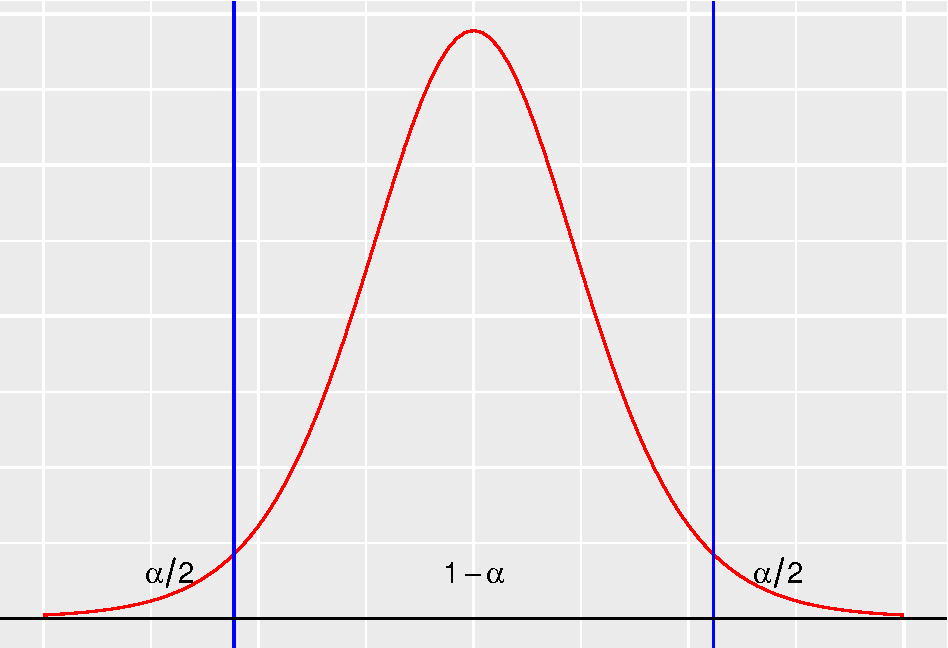
\includegraphics{2MLR_files/figure-latex/unnamed-chunk-37-1.pdf}

(Blue lines at \(\pm t_{\alpha/2,n-p}\).)

\begin{center}\rule{0.5\linewidth}{0.5pt}\end{center}

Inserting
\(T_j =\frac{\hat{\beta}_j-\beta_j}{\sqrt{c_{jj}}\hat{\sigma}}\) and
solving so \(\beta_j\) is in the middle gives:
\[ P(\hat{\beta}_j-t_{\alpha/2,n-p}\sqrt{c_{jj}}\hat{\sigma}
\le \beta_j \le \hat{\beta}_j+t_{\alpha/2,n-p}\sqrt{c_{jj}}\hat{\sigma})=1-\alpha\]

\begin{center}\rule{0.5\linewidth}{0.5pt}\end{center}

A \((1-\alpha)\)\% CI for \(\beta_j\) is when we insert numerical values
for the upper and lower limits:
\([\hat{\beta}_j-t_{\alpha/2,n-p}\sqrt{c_{jj}}\hat{\sigma},\hat{\beta}_j+t_{\alpha/2,n-p}\sqrt{c_{jj}}\hat{\sigma}]\).

CIs can be found in R using \texttt{confint} on an \texttt{lm} object.
(Here dummy variable coding is used for \texttt{location}, with average
as reference location.)

\small

\begin{Shaded}
\begin{Highlighting}[]
\FunctionTok{library}\NormalTok{(gamlss.data)}
\NormalTok{fit }\OtherTok{=} \FunctionTok{lm}\NormalTok{(rent }\SpecialCharTok{\textasciitilde{}}\NormalTok{ area }\SpecialCharTok{+}\NormalTok{ location }\SpecialCharTok{+}\NormalTok{ bath }\SpecialCharTok{+}\NormalTok{ kitchen }\SpecialCharTok{+}\NormalTok{ cheating, }\AttributeTok{data =}\NormalTok{ rent99)}
\FunctionTok{confint}\NormalTok{(fit)}
\end{Highlighting}
\end{Shaded}

\begin{verbatim}
##                  2.5 %      97.5 %
## (Intercept) -44.825534   0.8788739
## area          4.354674   4.8029443
## location2    28.579849  49.9405909
## location3    92.970636 159.1443278
## bath1        52.076412  96.0311030
## kitchen1     94.907671 145.9621578
## cheating1   144.427555 178.4000215
\end{verbatim}

\normalsize

\begin{center}\rule{0.5\linewidth}{0.5pt}\end{center}

\textbf{Q} (and A):

\begin{enumerate}
\def\labelenumi{\arabic{enumi}.}
\tightlist
\item
  What is the interpretation of a 95\% confidence interval?
\item
  Does the CI for \(\hat{\beta}_{\text{area}}\) change if we change the
  regression model (e.g.~not include \texttt{cheating})?
\item
  How can we in practice find a CI for \texttt{location1} (average
  location) - when that is not printed above? (Yes, may use formula, but
  in R without maths?)
\item
  What if we go for an asymptotic confidence interval - what will
  change?
\end{enumerate}

\begin{center}\rule{0.5\linewidth}{0.5pt}\end{center}

\hypertarget{prediction-intervals}{%
\subsection{Prediction intervals}\label{prediction-intervals}}

Remember, one aim for regression was to ``construct a model to predict
the reponse from a set of (one or several) explanatory variables- more
or less black box''.

Assume we want to make a prediction (of the response - often called
\(Y_0\)) given specific values for the covariates - often called
\({\bf x}_0\). An intuitive point estimate is
\(\hat{Y}_0={\bf x}_0^T \hat{\beta}\) - but to give a hint of the
uncertainty in this prediction we also want to present a prediction
interval for the \(Y_0\).

\begin{center}\rule{0.5\linewidth}{0.5pt}\end{center}

To arrive at such an estimate we start with the difference between the
unobserved response \(Y_0\) (for a given covariate vector \({\bf x}_0\))
and the point prediction \(\hat{Y}_0\), \(Y_0-\hat{Y}_0\). First, we
assume that the unobserved response at covariate \({\bf x}_0\) is
independent of our previous observations and follows the same
distibution, that is \(Y_0 \sim N({\bf x}_0^T \beta,\sigma^2)\).
Further,

\[\hat{Y}_0={\bf x}_0^T \hat{\beta} \sim N({\bf x}_0^T \beta,\sigma^2 {\bf x}_0^T({\bf X}^T{\bf X})^{-1}{\bf x}_0).\]

Then, for \(Y_0-{\bf x}_0^T \hat{\beta}\) we have
\[\text{E}(Y_0-{\bf x}_0^T \hat{\beta})=0 \text{ and } \text{Var}(Y_0-{\bf x}_0^T \hat{\beta})=\text{Var}(Y_0)+\text{Var}({\bf x}_0^T \hat{\beta})=\sigma^2+\sigma^2{\bf x}_0^T({\bf X}^T{\bf X})^{-1}{\bf x}_0\]
so that
\[Y_0-{\bf x}_0^T \hat{\beta}\sim N(0,\sigma^2 (1+{\bf x}_0^T({\bf X}^T{\bf X})^{-1}{\bf x}_0)) \]
---

Inserting our REML-estimate for \(\sigma^2\) gives

\[T=\frac{Y_0-{\bf x}_0^T \hat{\beta}}{\hat{\sigma}\sqrt{1+{\bf x}_0^T({\bf X}^T{\bf X})^{-1}{\bf x}_0}}\sim t_{n-p}.\]

Then, we start with
\[ P(-t_{\alpha/2,n-p}\le \frac{Y_0-{\bf x}_0^T \hat{\beta}}{\hat{\sigma}\sqrt{1+{\bf x}_0^T({\bf X}^T{\bf X})^{-1}{\bf x}_0}} \le t_{\alpha/2,n-p})=1-\alpha\]
and solve so that \(Y_0\) is in the middle, which gives
\[P({\bf x}_0^T \hat{\beta}-t_{\alpha/2,n-p}\hat{\sigma}\sqrt{1+{\bf x}_0^T({\bf X}^T{\bf X})^{-1}{\bf x}_0} \le Y_0 \le {\bf x}_0^T \hat{\beta}+t_{\alpha/2,n-p}\hat{\sigma}\sqrt{1+{\bf x}_0^T({\bf X}^T{\bf X})^{-1}{\bf x}_0})=1-\alpha\]

\begin{center}\rule{0.5\linewidth}{0.5pt}\end{center}

A \((1-\alpha)\)\% PI for \(Y_0\) is when we insert numerical values for
the upper and lower limits:
\([{\bf x}_0^T \hat{\beta}-t_{\alpha/2,n-p}\hat{\sigma}\sqrt{1+{\bf x}_0^T({\bf X}^T{\bf X})^{-1}{\bf x}_0}, {\bf x}_0^T \hat{\beta}+t_{\alpha/2,n-p}\hat{\sigma}\sqrt{1+{\bf x}_0^T({\bf X}^T{\bf X})^{-1}{\bf x}_0}]\).

\begin{center}\rule{0.5\linewidth}{0.5pt}\end{center}

PIs can be found in R using \texttt{predict} on an \texttt{lm} object,
but make sure that \texttt{newdata} is a \texttt{data.frame} with the
same names as the original data. We want to predict the rent - with PI -
for an appartment with area 50, location 2 (``good''), nice bath and
kitchen and with central heating.

\begin{Shaded}
\begin{Highlighting}[]
\FunctionTok{library}\NormalTok{(gamlss.data)}
\NormalTok{fit }\OtherTok{=} \FunctionTok{lm}\NormalTok{(rent }\SpecialCharTok{\textasciitilde{}}\NormalTok{ area }\SpecialCharTok{+}\NormalTok{ location }\SpecialCharTok{+}\NormalTok{ bath }\SpecialCharTok{+}\NormalTok{ kitchen }\SpecialCharTok{+}\NormalTok{ cheating, }\AttributeTok{data =}\NormalTok{ rent99)}
\NormalTok{newobs }\OtherTok{=}\NormalTok{ rent99[}\DecValTok{1}\NormalTok{, ]}
\NormalTok{newobs[}\DecValTok{1}\NormalTok{, ] }\OtherTok{=} \FunctionTok{c}\NormalTok{(}\ConstantTok{NA}\NormalTok{, }\ConstantTok{NA}\NormalTok{, }\DecValTok{50}\NormalTok{, }\ConstantTok{NA}\NormalTok{, }\DecValTok{2}\NormalTok{, }\DecValTok{1}\NormalTok{, }\DecValTok{1}\NormalTok{, }\DecValTok{1}\NormalTok{, }\ConstantTok{NA}\NormalTok{)}
\FunctionTok{predict}\NormalTok{(fit, }\AttributeTok{newdata =}\NormalTok{ newobs, }\AttributeTok{interval =} \StringTok{"prediction"}\NormalTok{, }\AttributeTok{type =} \StringTok{"response"}\NormalTok{)}
\end{Highlighting}
\end{Shaded}

\begin{verbatim}
##        fit      lwr      upr
## 1 602.1298 315.5353 888.7243
\end{verbatim}

\begin{center}\rule{0.5\linewidth}{0.5pt}\end{center}

\textbf{Q} (and A):

\begin{enumerate}
\def\labelenumi{\arabic{enumi}.}
\tightlist
\item
  When is a prediction interval of interest?
\item
  Explain the result from \texttt{predict} above.
\item
  What is the interpretation of a 95\% prediction interval?
\item
  What will change if want an asymptotic interval?
\end{enumerate}

\begin{center}\rule{0.5\linewidth}{0.5pt}\end{center}

\hypertarget{single-hypothesis-testing-set-up}{%
\subsection{Single hypothesis testing
set-up}\label{single-hypothesis-testing-set-up}}

In single hypothesis testing we are interesting in testing one null
hypothesis against an alternative hypothesis. In linear regression the
hypothesis is often about a regression parameter \(\beta_j\):
\[H_0: \beta_j=0 \text{ vs. } H_1: \beta_j\neq 0\]

Remark: we implicitly say that our test is done given that the other
variables are present in the model, that is, the other \(\beta_i\)s
(\(j\neq i\)) are not zero.

\#\#\#Two types of errors:

\begin{itemize}
\item
  ``Reject \(H_0\) when \(H_0\) is true''=``false positives'' = ``type I
  error'' =``miscarriage of justice''. These are our \emph{fake news},
  which are very important for us to avoid.
\item
  ``Fail to reject \(H_0\) when \(H_1\) is true (and \(H_0\) is
  false)''=``false negatives'' = ``type II error''= ``guilty criminal go
  free''.
\end{itemize}

\begin{center}\rule{0.5\linewidth}{0.5pt}\end{center}

We choose to reject \(H_0\) at some significance level \(\alpha\) if the
\(p\)-value of the test (see below) is smaller than the chosen
significance level. We say that : Type I error is ``controlled'' at
significance level \(\alpha\), which means that the probability of
miscarriage of justice (Type I error) does not exceed \(\alpha\).

\textbf{Q}: Draw a 2 by 2 table showing the connection between

\begin{itemize}
\tightlist
\item
  ``truth'' (\(H_0\) true or \(H_0\) false) - rows in the table, and
\item
  ``action'' (reject \(H_0\) and accept \(H_0\)) - columns in the table,
\end{itemize}

and place the two types of errors in the correct position within the
table.

What else should be written in the last two cells?

\begin{center}\rule{0.5\linewidth}{0.5pt}\end{center}

\hypertarget{hypothesis-test-on-beta_j-t-test}{%
\subsubsection{\texorpdfstring{Hypothesis test on \(\beta_j\)
(t-test)}{Hypothesis test on \textbackslash beta\_j (t-test)}}\label{hypothesis-test-on-beta_j-t-test}}

In linear regression models our test statistic for testing
\(H_0: \beta_j=0\) is
\[T_0=\frac{\hat{\beta}_j-0}{\sqrt{c_{jj}}\hat{\sigma}}\sim t_{n-p}\]
where \(c_{jj}\hat{\sigma}^2=\widehat{\text{Var}}(\hat{\beta}_j)\).

Inserted observed values (and estimates) we have \(t_0\).

We would in a two-sided setting reject \(H_0\) for large values of
\(\text{abs}(t_0)\). We may rely on calculating a \(p\)-value.

\textbf{Q}: what if we want an asymptotic test statistics?

\begin{center}\rule{0.5\linewidth}{0.5pt}\end{center}

\hypertarget{the-p-value}{%
\subsubsection{The p-value}\label{the-p-value}}

A p-value is a test statistic satisfying \(0 \leq p({\bf Y}) \leq 1\)
for every vector of observations \({\bf Y}\).

\begin{itemize}
\tightlist
\item
  Small values give evidence that \(H_1\) is true.
\item
  In single hypothesis testing, if the p-value is less than the chosen
  significance level (chosen upper limit for the probability of
  committing a type I error), then we reject the null hypothesis,
  \(H_0\). The chosen significance level is often referred to as
  \(\alpha\).
\item
  A p-value is \emph{valid} if
  \[ P(p({\bf Y}) \leq \alpha) \leq \alpha\] for all \(\alpha\),
  \(0 \leq \alpha \leq 1\), whenever \(H_0\) is true, that is, if the
  \(p\)-value is valid, rejection on the basis of the \(p\)-value
  ensures that the probability of type I error does not exceed
  \(\alpha\).
\item
  If \(P(p({\bf Y}) \leq \alpha) = \alpha\) for all \(\alpha\),
  \(0 \leq \alpha \leq 1\), the \(p\)-value is called an \emph{exact}
  p-value.
\end{itemize}

\begin{center}\rule{0.5\linewidth}{0.5pt}\end{center}

In our linear regression we use the \(t\)-distibution to calculate
p-values for our two-sided test situation \(H_0: \beta_j=0\)
vs.~\(H_1: \beta_j \neq 0\). Assume we have observed that our test
statistic \(T_0\) takes the numerical value \(t_0\). Since the
\(t\)-distribution is symmetric around \(0\) we have

\[p\text{-value}=P(T_0>\text{abs}(t_0))+P(T_0<-\text{abs}(t_0))=2\cdot P(T_0>\text{abs}(t_0)).\]

We reject \(H_0\) if our calculated \(p\)-value is below our chosen
signficance level. We often choose as significance level
\(\alpha=0.05\).

\textbf{Q}: what if we want an asymptotic \(p\)-value?

\begin{center}\rule{0.5\linewidth}{0.5pt}\end{center}

\hypertarget{munich-rent-index-hypothesis-test}{%
\subsubsection{Munich rent index hypothesis
test}\label{munich-rent-index-hypothesis-test}}

We look at print-out using \texttt{summary} from fitting \texttt{lm}.

\footnotesize

\begin{Shaded}
\begin{Highlighting}[]
\FunctionTok{library}\NormalTok{(gamlss.data)}
\FunctionTok{colnames}\NormalTok{(rent99)}
\end{Highlighting}
\end{Shaded}

\begin{verbatim}
## [1] "rent"     "rentsqm"  "area"     "yearc"    "location" "bath"     "kitchen" 
## [8] "cheating" "district"
\end{verbatim}

\begin{Shaded}
\begin{Highlighting}[]
\NormalTok{fit }\OtherTok{=} \FunctionTok{lm}\NormalTok{(rent }\SpecialCharTok{\textasciitilde{}}\NormalTok{ area }\SpecialCharTok{+}\NormalTok{ location }\SpecialCharTok{+}\NormalTok{ bath }\SpecialCharTok{+}\NormalTok{ kitchen }\SpecialCharTok{+}\NormalTok{ cheating, }\AttributeTok{data =}\NormalTok{ rent99)}
\FunctionTok{summary}\NormalTok{(fit)}
\end{Highlighting}
\end{Shaded}

\begin{verbatim}
## 
## Call:
## lm(formula = rent ~ area + location + bath + kitchen + cheating, 
##     data = rent99)
## 
## Residuals:
##     Min      1Q  Median      3Q     Max 
## -633.41  -89.17   -6.26   82.96 1000.76 
## 
## Coefficients:
##             Estimate Std. Error t value Pr(>|t|)    
## (Intercept) -21.9733    11.6549  -1.885   0.0595 .  
## area          4.5788     0.1143  40.055  < 2e-16 ***
## location2    39.2602     5.4471   7.208 7.14e-13 ***
## location3   126.0575    16.8747   7.470 1.04e-13 ***
## bath1        74.0538    11.2087   6.607 4.61e-11 ***
## kitchen1    120.4349    13.0192   9.251  < 2e-16 ***
## cheating1   161.4138     8.6632  18.632  < 2e-16 ***
## ---
## Signif. codes:  0 '***' 0.001 '**' 0.01 '*' 0.05 '.' 0.1 ' ' 1
## 
## Residual standard error: 145.2 on 3075 degrees of freedom
## Multiple R-squared:  0.4504, Adjusted R-squared:  0.4494 
## F-statistic:   420 on 6 and 3075 DF,  p-value: < 2.2e-16
\end{verbatim}

\normalsize

\begin{center}\rule{0.5\linewidth}{0.5pt}\end{center}

\textbf{Q} (and A):

\begin{enumerate}
\def\labelenumi{\arabic{enumi}.}
\tightlist
\item
  Where is hypothesis testing performed here, and which are the
  hypotheses rejected at level \(0.01\)?
\item
  Will the test statistics and \(p\)-values change if we change the
  regression model?
\item
  What is the relationship between performing an hypothesis test and
  constructing a CI interval? Remember:
\end{enumerate}

\begin{Shaded}
\begin{Highlighting}[]
\FunctionTok{library}\NormalTok{(gamlss.data)}
\NormalTok{fit }\OtherTok{=} \FunctionTok{lm}\NormalTok{(rent }\SpecialCharTok{\textasciitilde{}}\NormalTok{ area }\SpecialCharTok{+}\NormalTok{ location }\SpecialCharTok{+}\NormalTok{ bath }\SpecialCharTok{+}\NormalTok{ kitchen }\SpecialCharTok{+}\NormalTok{ cheating, }\AttributeTok{data =}\NormalTok{ rent99)}
\FunctionTok{confint}\NormalTok{(fit)}
\end{Highlighting}
\end{Shaded}

\begin{verbatim}
##                  2.5 %      97.5 %
## (Intercept) -44.825534   0.8788739
## area          4.354674   4.8029443
## location2    28.579849  49.9405909
## location3    92.970636 159.1443278
## bath1        52.076412  96.0311030
## kitchen1     94.907671 145.9621578
## cheating1   144.427555 178.4000215
\end{verbatim}

\begin{center}\rule{0.5\linewidth}{0.5pt}\end{center}

\hypertarget{testing-linear-hypotheses-in-regression}{%
\subsection{Testing linear hypotheses in
regression}\label{testing-linear-hypotheses-in-regression}}

We study a normal linear regression model with \(p=k+1\) covariates, and
refer to this as model A (the larger model). We then want to investigate
the null and alternative hypotheses of the following type(s):
\begin{eqnarray*}
 H_0: \beta_{j}&=&0 \text{ vs. } H_1:\beta_j\neq 0\\
 H_0: \beta_{1}&=&\beta_{2}=\beta_{3}=0 \text{ vs. } H_1:\text{ at least one of these }\neq 0\\
 H_0: \beta_{1}&=&\beta_{2}=\cdots=\beta_{k}=0 \text{ vs. } H_1:\text{ at least one of these }\neq 0\\
 \end{eqnarray*}

We call the restricted model (when the null hypotesis is true) model B,
or the smaller model.

\begin{center}\rule{0.5\linewidth}{0.5pt}\end{center}

These null hypotheses and alternative hypotheses can all be rewritten as
a linear hypothesis
\[H_0: {\bf C}{\bf \beta}={\bf d} \text{ vs. } {\bf C}{\bf \beta}\neq {\bf d} \]
by specifying \({\bf C}\) to be a \(r \times p\) matrix and \({\bf d}\)
to be a column vector of length \(r\).

The test statistic for performing the test is called \(F_{obs}\) and can
be formulated in two ways: \begin{eqnarray}
F_{obs}&=&\frac{\frac{1}{r} (SSE_{H_0}-SSE)}{\frac{SSE}{n-p}} \label{Fobsnested}\\
F_{obs}&=&\frac{1}{r}({\bf C}\hat{{\bf \beta}}-{\bf d})^{\text T}[\hat{\sigma}^2 {\bf C}({\bf X}^{\text T}{\bf X})^{-1}{\bf C}^{\text T}]^{-1}({\bf C}\hat{{\bf \beta}}-{\bf d}) \label{FobsCbeta}
\end{eqnarray} where \(SSE\) is from the larger model A, \(SSE_{H_0}\)
from the smaller model B, and \(\hat{{\bf \beta}}\) and
\(\hat{\sigma}^2\) are estimators from the larger model A.

\begin{center}\rule{0.5\linewidth}{0.5pt}\end{center}

\hypertarget{testing-a-set-of-parameters---what-is-bf-c-and-bf-d}{%
\subsubsection{\texorpdfstring{Testing a set of parameters - what is
\({\bf C}\) and
\({\bf d}\)?}{Testing a set of parameters - what is \{\textbackslash bf C\} and \{\textbackslash bf d\}?}}\label{testing-a-set-of-parameters---what-is-bf-c-and-bf-d}}

We consider a regression model with intercept and five covariates,
\(x_1, \ldots, x_5\). Assume that we want to know if the covariates
\(x_3\), \(x_4\), and \(x_5\) can be dropped (due to the fact that none
of the corresponding \(\beta_j\)s are different from zero). This means
that we want to test:

\[H_0: \beta_{3}=\beta_{4}=\beta_{5}=0 \text{ vs. } H_1:\text{ at least one of these }\neq 0\]
This means that our \({\bf C}\) is a \(3\times 6\) matrix and
\({\bf d}\) a \(3 \times 1\) column vector
\[ {\bf C}=\begin{pmatrix} 0 &0 &0 &1 &0&0 \\
0&0&0&0&1&0\\
0&0&0&0&0& 1\\
\end{pmatrix} \text{ and } 
{\bf d} =\begin{pmatrix} 0\\0\\0\\ \end{pmatrix}\]

\begin{center}\rule{0.5\linewidth}{0.5pt}\end{center}

\hypertarget{testing-one-regression-parameter}{%
\subsubsection{Testing one regression
parameter}\label{testing-one-regression-parameter}}

If we set \({\bf C}=(0,1, 0, \cdots, 0)^T\), a row vector with 1 in
position 2 and 0 elsewhere, and \({\bf d}=(0,0,\ldots,0)\), a column
vector with 0s, then we test
\[ H_0: \beta_1=0 \text{ vs. } H_1: \beta_1\neq 0.\] Now
\({\bf C}\hat{\beta}=\beta_1\) and
\({\bf C}({\bf X}^{\text T}{\bf X})^{-1}{\bf C}^{\text T}=c_{11}\), so
that \(F_{obs}\) then is equal to the square of the \(t\)-statistics for
testing a single regression parameter.
\[F_{obs}=(\hat{\beta}_1-0)^T[\hat{\sigma}^2 c_{jj}]^{-1}(\hat{\beta}_1-0)=T_1^2\]

Repeat the argument with \(\beta_j\) instead of \(\beta_1\).

Remark: Remember that \(T_{\nu}^2=F_{1,\nu}\).

\begin{center}\rule{0.5\linewidth}{0.5pt}\end{center}

\hypertarget{testing-significance-of-the-regression}{%
\subsubsection{Testing ``significance of the
regression''}\label{testing-significance-of-the-regression}}

If we set \({\bf C}=(0,1,1, \cdots ,1)^T\), a row vector with 0 in
position 1 and 0 elsewhere, and \({\bf d}=0\), a scalar, then we test
\[ H_0: \beta_1=\beta_2=\cdots= \beta_k =0 \text{ vs. } H_1: \text{at least one different from zero}.\]
This means we test if at least one of the regression parameters (in
addition to the intercept) is different from 0. The small model is then
the model with only the intercept, and for this model the SSE\(_{H_0}\)
is equal to SST (sums of squares total, see below). Let SSE be the
sums-of-squares of errors for the full model. If we have \(k\)
regression parameters (in addition to the intercept) then the
F-statistic becomes
\[ F_{obs}=\frac{\frac{1}{k}(\text{SST}-\text{SSE})}{\frac{\text{SSE}}{n-p}}\]
with \(k\) and \(n-p\) degrees of freedom under \(H_0\).

\begin{center}\rule{0.5\linewidth}{0.5pt}\end{center}

\footnotesize

\begin{Shaded}
\begin{Highlighting}[]
\FunctionTok{library}\NormalTok{(gamlss.data)}
\NormalTok{fit }\OtherTok{=} \FunctionTok{lm}\NormalTok{(rent }\SpecialCharTok{\textasciitilde{}}\NormalTok{ area }\SpecialCharTok{+}\NormalTok{ location }\SpecialCharTok{+}\NormalTok{ bath }\SpecialCharTok{+}\NormalTok{ kitchen }\SpecialCharTok{+}\NormalTok{ cheating, }\AttributeTok{data =}\NormalTok{ rent99)}
\FunctionTok{summary}\NormalTok{(fit)}
\end{Highlighting}
\end{Shaded}

\begin{verbatim}
## 
## Call:
## lm(formula = rent ~ area + location + bath + kitchen + cheating, 
##     data = rent99)
## 
## Residuals:
##     Min      1Q  Median      3Q     Max 
## -633.41  -89.17   -6.26   82.96 1000.76 
## 
## Coefficients:
##             Estimate Std. Error t value Pr(>|t|)    
## (Intercept) -21.9733    11.6549  -1.885   0.0595 .  
## area          4.5788     0.1143  40.055  < 2e-16 ***
## location2    39.2602     5.4471   7.208 7.14e-13 ***
## location3   126.0575    16.8747   7.470 1.04e-13 ***
## bath1        74.0538    11.2087   6.607 4.61e-11 ***
## kitchen1    120.4349    13.0192   9.251  < 2e-16 ***
## cheating1   161.4138     8.6632  18.632  < 2e-16 ***
## ---
## Signif. codes:  0 '***' 0.001 '**' 0.01 '*' 0.05 '.' 0.1 ' ' 1
## 
## Residual standard error: 145.2 on 3075 degrees of freedom
## Multiple R-squared:  0.4504, Adjusted R-squared:  0.4494 
## F-statistic:   420 on 6 and 3075 DF,  p-value: < 2.2e-16
\end{verbatim}

\normalsize

\textbf{Q} (and A): Is the regression significant?

\begin{center}\rule{0.5\linewidth}{0.5pt}\end{center}

\hypertarget{relation-to-wald-test}{%
\subsubsection{Relation to Wald test}\label{relation-to-wald-test}}

Since \(\text{Cov}(\hat{\beta})=\sigma^2 ({\bf X}^T{\bf X})^{-1}\), then
\(\text{Cov}({\bf C}\hat{\beta})={\bf C}\sigma^2({\bf X}^T{\bf X})^{-1}{\bf C}^T\),
so that \({\bf C}\hat{\sigma}^2({\bf X}^T{\bf X})^{-1}{\bf C}^T\) can be
seen as an estimate of \(\text{Cov}({\bf C}\hat{\beta})\). Therefore,
\(F_{obs}\) can be written

\[F_{obs}=\frac{1}{r}({\bf C}\hat{{\bf \beta}}-{\bf d})^{\text T}[\widehat{\text{Cov}}({\bf C}\hat{\beta})]^{-1}({\bf C}\hat{{\bf \beta}}-{\bf d})=\frac{1}{r}W\]
where \(W\) is a socalled Wald test. It is known that \(W\sim \chi^2_r\)
asymptotically as \(n\) becomes large. We will study the Wald test in
more detail later in this course.

\begin{center}\rule{0.5\linewidth}{0.5pt}\end{center}

\hypertarget{asymptotic-result}{%
\subsubsection{Asymptotic result}\label{asymptotic-result}}

It can in general be shown that
\[r F_{r,n-p}\stackrel{n\rightarrow \infty}{\longrightarrow} \chi^2_r.\]
That is, if we have a random variable \(F\) that is distributed as
Fisher with \(r\) (numerator) and \(n-p\) (denominator) degrees of
freedom, then when \(n\) goes to infinity (\(p\) kept fixed), then
\(rF\) is approximately \(\chi^2\)-distributed with \(r\) degrees of
freedom.

Also, if our error terms are not normally distributed then we can assume
that when the number of observation becomes very large then
\(rF_{r,n-p}\) is approximately \(\chi^2_r\).

\hypertarget{introducing-deviance}{%
\section{Introducing deviance}\label{introducing-deviance}}

The deviance will replace the SSE (sums of squares of errors, aka
residual sums of squares) in the GLM setting, and now we take a first
look at the deviance, but to do that we first look at the likelihood
ratio test.

\begin{center}\rule{0.5\linewidth}{0.5pt}\end{center}

\hypertarget{the-likelihood-ratio-test}{%
\subsection{The likelihood ratio test}\label{the-likelihood-ratio-test}}

An alternative to the Wald test (based on the F-test shown previously)
is the likelihood ratio test (LRT), which compares the likelihood of
\emph{two models}.

We use the following notation. A: the larger model (this is \(H_1\)) and
B: the smaller model (under \(H_0\)), and the smaller model is nested
within the larger model (that is, B is a submodel of A).

\begin{itemize}
\tightlist
\item
  First we maximize the likelihood for model A (the larger model) and
  find the maximum likelihood parameter estimates \(\hat{\beta}_A\) and
  \(\tilde{\sigma}_A\). The maximum likelihood is achieved at this
  parameter estimate and is denoted
  \(L(\hat{\beta}_A, \tilde{\sigma}_A)\).
\item
  Then we maximize the likelihood for model B (the smaller model) and
  find the maximum likelihood parameter estimates \(\hat{\beta}_B\) and
  \(\tilde{\sigma}_B\). The maximum likelihood is achieved at this
  parameter estimate and is denoted
  \(L(\hat{\beta}_B,\tilde{\sigma}_B)\).
\end{itemize}

The likelihood of the larger model (A) will always be larger or equal to
the likelihood of the smaller model (B). Why?

\begin{center}\rule{0.5\linewidth}{0.5pt}\end{center}

The likelihood ratio statistic is defined as
\[- 2\ln \lambda=-2(\ln L(\hat{\beta}_B,\tilde{\sigma}_B)-\ln L(\hat{\beta}_A,\tilde{\sigma}_A)) \]
(so, \(-2\) times small minus large).

Under weak regularity conditions the test statistic is approximately
\(\chi^2\)-distributed with degrees of freedom equal the difference in
the number of parameters in the large and the small model. This is
general - and not related to the GLM! More about this result in TMA4295
Statistical Inference!

\(P\)-values are calculated in the upper tail of the
\(\chi^2\)-distribution.

Observe: to perform the test you need to fit both the small and the
large model.

Notice: \emph{asymptotically} the Wald and likelihood ratio test
statistics have the same distribution, but the value of the test
statistics might be different.

\begin{center}\rule{0.5\linewidth}{0.5pt}\end{center}

\hypertarget{example-munich-rent-data}{%
\subsubsection{Example: Munich rent
data}\label{example-munich-rent-data}}

\begin{itemize}
\tightlist
\item
  A (larger): model with \texttt{area}, \texttt{location} and
  \texttt{bath}.
\item
  B (smaller): model with \texttt{area} only.
\end{itemize}

\begin{Shaded}
\begin{Highlighting}[]
\FunctionTok{library}\NormalTok{(lmtest)}
\NormalTok{fitB }\OtherTok{\textless{}{-}} \FunctionTok{lm}\NormalTok{(rent }\SpecialCharTok{\textasciitilde{}}\NormalTok{ area, }\AttributeTok{data =}\NormalTok{ rent99)}
\NormalTok{fitA }\OtherTok{\textless{}{-}} \FunctionTok{update}\NormalTok{(fitB, . }\SpecialCharTok{\textasciitilde{}}\NormalTok{ . }\SpecialCharTok{+}\NormalTok{ location }\SpecialCharTok{+}\NormalTok{ bath)}
\FunctionTok{lrtest}\NormalTok{(fitB, fitA)}
\end{Highlighting}
\end{Shaded}

\begin{verbatim}
## Likelihood ratio test
## 
## Model 1: rent ~ area
## Model 2: rent ~ area + location + bath
##   #Df LogLik Df  Chisq Pr(>Chisq)    
## 1   3 -19990                         
## 2   6 -19923  3 134.34  < 2.2e-16 ***
## ---
## Signif. codes:  0 '***' 0.001 '**' 0.01 '*' 0.05 '.' 0.1 ' ' 1
\end{verbatim}

\begin{Shaded}
\begin{Highlighting}[]
\FunctionTok{anova}\NormalTok{(fitB, fitA, }\AttributeTok{test =} \StringTok{"Chisq"}\NormalTok{)}
\end{Highlighting}
\end{Shaded}

\begin{verbatim}
## Analysis of Variance Table
## 
## Model 1: rent ~ area
## Model 2: rent ~ area + location + bath
##   Res.Df      RSS Df Sum of Sq  Pr(>Chi)    
## 1   3080 77646265                           
## 2   3077 74334393  3   3311872 < 2.2e-16 ***
## ---
## Signif. codes:  0 '***' 0.001 '**' 0.01 '*' 0.05 '.' 0.1 ' ' 1
\end{verbatim}

\begin{Shaded}
\begin{Highlighting}[]
\FunctionTok{anova}\NormalTok{(fitB, fitA)}
\end{Highlighting}
\end{Shaded}

\begin{verbatim}
## Analysis of Variance Table
## 
## Model 1: rent ~ area
## Model 2: rent ~ area + location + bath
##   Res.Df      RSS Df Sum of Sq      F    Pr(>F)    
## 1   3080 77646265                                  
## 2   3077 74334393  3   3311872 45.697 < 2.2e-16 ***
## ---
## Signif. codes:  0 '***' 0.001 '**' 0.01 '*' 0.05 '.' 0.1 ' ' 1
\end{verbatim}

Observe that the LRT can be performed using \texttt{anova} with
`test=``Chisq''.

\begin{center}\rule{0.5\linewidth}{0.5pt}\end{center}

\hypertarget{deviance}{%
\subsection{Deviance}\label{deviance}}

The \emph{deviance} (new!) is used to assess model fit and also for
model choice, and is based on the likelihood ratio test statistic. It is
used for all GLMs in general - and replaces using SSE in multiple linear
regression.

First: a covariate pattern is a unique combination of the covariates in
our model, for continuous covariates we often have \(n\) covariate
patterns if we have \(n\) observations. Let us assume that for now.

\textbf{Saturated model:} If we were to provide a perfect fit to our
data. This means that we have \(\hat{\mu}_i=y_i\). So, each observation
is given its own parameter.

\textbf{Candidate model:} The model that we are investigated can be
thought of as a \emph{candidate} model. Then we maximize the likelihood
and get \(\hat{\beta}\).

The \emph{deviance} is then defined as the likelihood ratio statistic,
where we put the saturated model in place of the larger model A and our
candidate model in place of the smaller model B:

\[D=-2(\ln L(\text{candidate model})-\ln L(\text{saturated model}))\]

The deviance compares the proposed model to the saturated model, and
then ask ``can we use a more parsimonious model to describe the data as
well as the most general model does?''.

For the MLR it turns out that the deviance is
\[D=\frac{1}{\sigma^2} \sum_{i=1}^n (y_i-{\bf x}_i^T \hat{\boldsymbol\beta})^2=\frac{\text{SSE}}{\sigma^2}\]

This is sometimes called the \emph{scaled deviance} while the
\emph{unscaled deviance} is \(\phi D\), where \(\phi\) is the dispersion
parameter. For the normal model the unscaled deviance is thus
\(\sigma^2 D=\text{SSE}\).

Warning: both the scaled and unscaled deviance is referred to as the
deviance, and called \(D\) in different sources. Our textbook use the
scaled version, while R use the unscaled.

\hypertarget{analysis-of-variance-decomposition-and-coefficient-of-determination-r2}{%
\section{\texorpdfstring{Analysis of variance decomposition and
coefficient of determination,
\(R^2\)}{Analysis of variance decomposition and coefficient of determination, R\^{}2}}\label{analysis-of-variance-decomposition-and-coefficient-of-determination-r2}}

\hypertarget{sums-of-squares-decomposition}{%
\subsection{Sums-of-squares
decomposition}\label{sums-of-squares-decomposition}}

It is possible to decompose the total variability in the data, called
SST (sums-of-squares total), into a part that is explained by the
regression SSR (sums-of-squares regression), and a part that is not
explained by the regression SSE (sums-of-squares error, or really
residual).

Let \(\bar{Y}=\frac{1}{n}\sum_{i=1}^n Y_i\), and
\(\hat{Y}_i={\bf x}_i^T\hat{\beta}\). Then, \begin{align*} 
\text{SST}&=\text{SSR}+\text{SSE}\\ 
\text{SST}&=\sum_{i=1}^n (Y_i-\bar{Y})^2={\bf Y}^T({\bf I}-\frac{1}{n}{\bf 1 1}^T){\bf Y}\\
\text{SSR}&=\sum_{i=1}^n (\hat{Y}_i-\bar{Y})^2={\bf Y}^T({\bf H}-\frac{1}{n}{\bf 1 1}^T){\bf Y}\\
\text{SSE}&=\sum_{i=1}^n (Y_i-\hat{Y}_i)^2=\sum_{i=1}^n \hat{\varepsilon}_i^2={\bf Y}^T({\bf I}-{\bf H}){\bf Y}.\\
\end{align*} The proof can be found in Section 3.5 in our text book
Regression.

\begin{center}\rule{0.5\linewidth}{0.5pt}\end{center}

Based on this decomposition we may define the \emph{coefficient of
determination} (\(R^2\)) as the ratio between SSR and SST, that is
\[R^2=\text{SSR}/\text{SST}=1-\text{SSE}/\text{SST}\]

\begin{enumerate}
\def\labelenumi{\arabic{enumi}.}
\tightlist
\item
  The interpretation of this coefficient is that the closer it is to 1
  the better the fit to the data. If \(R^2=1\) then all residuals are
  zero - that is, perfect fit to the data.
\item
  In a simple linear regression the \(R^2\) equals the squared
  correlation coefficient between the reponse and the predictor. In
  multiple linear regression \(R^2\) is the squared correlation
  coefficient between the observed and predicted response.
\item
  If we have two models \(M_1\) and \(M_2\), where model \(M_2\) is a
  submodel of model \(M_1\), then \[ R^2_{M_1}\ge R^2_{M_2}.\] This can
  be explained from the fact that
  \(\text{SSE}_{M_1}\le \text{SSE}_{M_2}\).
\end{enumerate}

\begin{center}\rule{0.5\linewidth}{0.5pt}\end{center}

\hypertarget{analysis-of-variance-tables---with-emphasis-on-sequential-type-i-anova}{%
\subsection{Analysis of variance tables - with emphasis on sequential
Type I
ANOVA}\label{analysis-of-variance-tables---with-emphasis-on-sequential-type-i-anova}}

It is possible to call the function \texttt{anova} on an
\texttt{lm}-object. What does that function do?

\begin{Shaded}
\begin{Highlighting}[]
\FunctionTok{library}\NormalTok{(gamlss.data)}
\NormalTok{fit }\OtherTok{=} \FunctionTok{lm}\NormalTok{(rent }\SpecialCharTok{\textasciitilde{}}\NormalTok{ area }\SpecialCharTok{+}\NormalTok{ location }\SpecialCharTok{+}\NormalTok{ bath }\SpecialCharTok{+}\NormalTok{ kitchen }\SpecialCharTok{+}\NormalTok{ cheating, }\AttributeTok{data =}\NormalTok{ rent99)}
\FunctionTok{anova}\NormalTok{(fit)}
\end{Highlighting}
\end{Shaded}

\begin{verbatim}
## Analysis of Variance Table
## 
## Response: rent
##             Df   Sum Sq  Mean Sq  F value    Pr(>F)    
## area         1 40299098 40299098 1911.765 < 2.2e-16 ***
## location     2  1635047   817524   38.783 < 2.2e-16 ***
## bath         1  1676825  1676825   79.547 < 2.2e-16 ***
## kitchen      1  2196952  2196952  104.222 < 2.2e-16 ***
## cheating     1  7317894  7317894  347.156 < 2.2e-16 ***
## Residuals 3075 64819547    21080                       
## ---
## Signif. codes:  0 '***' 0.001 '**' 0.01 '*' 0.05 '.' 0.1 ' ' 1
\end{verbatim}

\begin{center}\rule{0.5\linewidth}{0.5pt}\end{center}

What is produced is a \emph{sequential} table of \emph{the reductions in
residual sum of squares (SSE) as each term in the regression formula is
added in turn}. This type of ANOVA is often referred to as ``Type I''
(not to be confused with type I errors).

We can produce the same table by fitting larger and larger regression
models.

\begin{Shaded}
\begin{Highlighting}[]
\FunctionTok{library}\NormalTok{(gamlss.data)}
\NormalTok{fit }\OtherTok{=} \FunctionTok{lm}\NormalTok{(rent }\SpecialCharTok{\textasciitilde{}}\NormalTok{ area }\SpecialCharTok{+}\NormalTok{ location }\SpecialCharTok{+}\NormalTok{ bath }\SpecialCharTok{+}\NormalTok{ kitchen }\SpecialCharTok{+}\NormalTok{ cheating, }\AttributeTok{data =}\NormalTok{ rent99)}
\NormalTok{fit0 }\OtherTok{\textless{}{-}} \FunctionTok{lm}\NormalTok{(rent }\SpecialCharTok{\textasciitilde{}} \DecValTok{1}\NormalTok{, }\AttributeTok{data =}\NormalTok{ rent99)}
\NormalTok{fit1 }\OtherTok{\textless{}{-}} \FunctionTok{update}\NormalTok{(fit0, . }\SpecialCharTok{\textasciitilde{}}\NormalTok{ . }\SpecialCharTok{+}\NormalTok{ area)}
\NormalTok{fit2 }\OtherTok{\textless{}{-}} \FunctionTok{update}\NormalTok{(fit1, . }\SpecialCharTok{\textasciitilde{}}\NormalTok{ . }\SpecialCharTok{+}\NormalTok{ location)}
\NormalTok{fit3 }\OtherTok{\textless{}{-}} \FunctionTok{update}\NormalTok{(fit2, . }\SpecialCharTok{\textasciitilde{}}\NormalTok{ . }\SpecialCharTok{+}\NormalTok{ bath)}
\NormalTok{fit4 }\OtherTok{\textless{}{-}} \FunctionTok{update}\NormalTok{(fit3, . }\SpecialCharTok{\textasciitilde{}}\NormalTok{ . }\SpecialCharTok{+}\NormalTok{ kitchen)}
\NormalTok{fit5 }\OtherTok{\textless{}{-}} \FunctionTok{update}\NormalTok{(fit4, . }\SpecialCharTok{\textasciitilde{}}\NormalTok{ . }\SpecialCharTok{+}\NormalTok{ cheating)}
\FunctionTok{anova}\NormalTok{(fit0, fit1, fit2, fit3, fit4, fit5, }\AttributeTok{test =} \StringTok{"F"}\NormalTok{)}
\end{Highlighting}
\end{Shaded}

\begin{verbatim}
## Analysis of Variance Table
## 
## Model 1: rent ~ 1
## Model 2: rent ~ area
## Model 3: rent ~ area + location
## Model 4: rent ~ area + location + bath
## Model 5: rent ~ area + location + bath + kitchen
## Model 6: rent ~ area + location + bath + kitchen + cheating
##   Res.Df       RSS Df Sum of Sq        F    Pr(>F)    
## 1   3081 117945363                                    
## 2   3080  77646265  1  40299098 1911.765 < 2.2e-16 ***
## 3   3078  76011217  2   1635047   38.783 < 2.2e-16 ***
## 4   3077  74334393  1   1676825   79.547 < 2.2e-16 ***
## 5   3076  72137441  1   2196952  104.222 < 2.2e-16 ***
## 6   3075  64819547  1   7317894  347.156 < 2.2e-16 ***
## ---
## Signif. codes:  0 '***' 0.001 '**' 0.01 '*' 0.05 '.' 0.1 ' ' 1
\end{verbatim}

\begin{Shaded}
\begin{Highlighting}[]
\CommentTok{\# anova(fit0,fit1) \# compare model 0 and 1 {-} NOT sequential}
\CommentTok{\# anova(fit0,fit5) \# compare model 0 and 5 {-} NOT sequential}
\end{Highlighting}
\end{Shaded}

If we had changed the order of adding the covariates to the model, then
our anova table would also change. You might check that if you want.

\begin{center}\rule{0.5\linewidth}{0.5pt}\end{center}

\#\#\#Details on the test \texttt{anova(fit)}

When running \texttt{anova} on one fitted regression the \(F\)-test in
\texttt{anova} is calculated as for ``testing linear hypotheses'' - but
with a slight twist. Our large model is still the full regression model
(from the fitted object), but the smaller model is replaced by the
\emph{the change from one model to the next}.

Let SSE be the sums-of-squares-error (residual sums of squares) from the
full (large, called A) model - this will be our denominator (as always).
For our rent example the denominator will be SSE/(n-p)=64819547/3075
(see print-out above).

However, for the numerator we are not comparing one small model with the
full (large) one, we are instead looking at the change in SSE between
two (smaller) models (calles model B1 and B2). So, now we have in the
numerator the difference in SSE between models B1 and B2, scaled with
the difference in number of parameters estimated in model B1 and B2
=``number in B2 minus in B1'' (which is the same as the difference in
degrees of freedom for the two models).

So, B1 could be the model with only intercept, and B2 could be the model
with intercept and area. Then we calculate the SSE for model B1 and for
model B2, and keep the difference (here 40299098). Then we count the
number of parameters in model B1 and model B2 and compute ``number in B2
minus in B1'' (here 1). We could istead have calculated the number of
degrees of freedom in the smaller model minus the number of degrees of
freedom for the larger model (which here is 1). Our numerator is then
40299098/1.

This means that the test statistics we use are:

\[ F_0=\frac{\frac{\text{SSE}_{B1}-\text{SSE}_{B2}}{\text{df}_{B1}-\text{df}_{B2}}}{\frac{\text{SSE}_A}{\text{df}_A}}\]
Remark: notice that the denominator is just the \(\hat{\sigma^2}\) from
the larger model A.

This makes our \(F\)-test statistic:
\(f_0=\frac{40299098/1}{64819547/3075}=1911.765\) (remember that we swap
from capital to small letters when we insert numerical values).

To produce a \(p\)-value to the test that
\[H_0: \text{"Model B1 and B2 are equally good" vs }H_1:\text{"Model B2 is better than B1}\]
and then the \(F\sim {\text{df}_{B1}-\text{df}_{B2},\text{df}_A}\). In
our example we compare to an F-distribution with 1 and 3075 degrees of
freedom. The \(p\)-value is the ``probability of observing a test
statistic at least as extreme as we have'' so we calculate the
\(p\)-value as \(P(F>f_0)\). This gives a \(p\)-value that is
practically 0.

If you then want to use the asymptotic version (relating to a chi-square
instead of the F), then multiply your F-statistic with
\(\text{df}_{B1}-\text{df}_{B2}\) and relate to a \(\chi^2\)
distribution with \(\text{df}_{B1}-\text{df}_{B2}\) degrees of freedom,
where \(\text{df}_{B1}-\text{df}_{B2}\) is the difference in number of
parameters in models B1 and B2. In our example
\(\text{df}_{B1}-\text{df}_{B2}=1\).

For the anova table we do this sequentially for all models from starting
with only intercept to the full model A. This means you need to
calculate SSE and df for models of all sizes to calculate lots of these
\(F_0\)s. Assume that we have 4 covariates that are added to the model,
and call the 5 possible models (given the order of adding the
covariates)

\begin{itemize}
\item
  model 1: model with only intercept
\item
  model 2: model with intercept and covariate 1
\item
  model 3: model with intercept and covariate 1 and covariate 2
\item
  model 4: model with intercept and covariate 1 and covariate 2 and
  covariate 3
\item
  model 5: model with intercept and covariate 1 and covariate 2 and
  covariate 3 and covariate 4
\end{itemize}

Fit a linear model (lm) for each model 1-5, and store SSE and degrees of
freedom=df (number of observations minus number of covariates estimated)
for each of the models. Call these SSE\(_1\) to SSE\(_5\) and df\(_1\)
to \(df\)\_5\$.

The anova output has columns: Df Sum Sq Mean Sq F value
Pr(\textgreater F) and one row for each covariate added to the model.

\begin{itemize}
\item
  model 2 vs model 1: Df=df\(_1\)-df\(_2\), Sum Sq=SSE\(_1\)-SSE\(_2\),
  Mean Sq=Sum Sq/Df, F value=(Mean Sq)/(SSE\(_5\)/df\(_5\))=\(f_0\),
  Pr(\textgreater F)=pvalue=\(P(F>f_0)\).
\item
  model 3 vs model 2: Df=df\(_2\)-df\(_3\), Sum Sq=SSE\(_2\)-SSE\(_3\),
  Mean Sq=Sum Sq/Df, F value=(Mean Sq)/(SSE\(_5\)/df\(_5\))=\(f_0\),
  Pr(\textgreater F)=pvalue=\(P(F>f_0)\).
\item
  model 4 vs model 3: Df=df\(_3\)-df\(_4\), Sum Sq=SSE\(_3\)-SSE\(_4\),
  Mean Sq=Sum Sq/Df, F value=(Mean Sq)/(SSE\(_5\)/df\(_5\))=\(f_0\),
  Pr(\textgreater F)=pvalue=\(P(F>f_0)\).
\item
  model 5 vs model 4: Df=df\(_4\)-df\(_5\), Sum Sq=SSE\(_4\)-SSE\(_5\),
  Mean Sq=Sum Sq/Df, F value=(Mean Sq)/(SSE\(_5\)/df\(_5\))=\(f_0\),
  Pr(\textgreater F)=pvalue=\(P(F>f_0)\).
\end{itemize}

In R the p-value is calculated as \texttt{1-pf(f0,Df)} or as
\texttt{1-pchisq(Df*f0,Df)} if the asymptotic chisquare distribution is
used.

So, this is what is presented - a sequential record of the effect of
adding a new covariate.

\textbf{Q}: what if you change the order of the covariates into the
model? Yes, then everything changes. That is the drawback of Type I
(sequential) thinking.

\textbf{Q}: What if one of the covariates is a factor? Then all
parameters of the factor (e.g.~all dummy variables) are tested in one
step (more in interactive lecture Problem 2).

\begin{center}\rule{0.5\linewidth}{0.5pt}\end{center}

A competing way of thinking is called \emph{type III ANOVA} and instead
of looking sequentially at adding terms, we (like in \texttt{summary})
calculated the contribution to a covariate (or factor) given that all
other covariates are present in the regression model. Type III ANOVA is
available from library \texttt{car} as function \texttt{Anova} (possible
to give type of anova as input).

\textbf{Check} : Take a look at the print-out from \texttt{summary} and
\texttt{anova} and observe that for our rent data the \(p\)-values for
each covariate are different due to the different nature of the \(H_0\)s
tested (sequential vs.~``all other present'').

If we had orthogonal columns for our different covariates the type I and
type III ANOVA tables would have been equal.

\hypertarget{optional-beyond-the-scope-of-this-course}{%
\paragraph{Optional (beyond the scope of this
course)}\label{optional-beyond-the-scope-of-this-course}}

There is also something called a type II ANOVA table, but that is mainly
important if we have interactions in our model, so we do not consider
that here. If you want to read more this blogplot
\url{https://www.r-bloggers.com/anova-\%E2\%80\%93-type-iiiiii-ss-explained/}
is a good read. And, in combination with different variants of dummy and
effect coding - read this:
\url{http://rstudio-pubs-static.s3.amazonaws.com/65059_586f394d8eb84f84b1baaf56ffb6b47f.html}.
A good read is
\href{https://link.springer.com/article/10.1023/A:1023260610025}{Langsrud
(2003): ANOVA for unbalanced data: Use Type II instead of Type III sums
of squares}.

\hypertarget{pointing-ahead}{%
\subsubsection{Pointing ahead}\label{pointing-ahead}}

For GLM the sequential analysis of variance (ANOVA) is replace by
analysis of deviance.

\hypertarget{model-selection}{%
\section{Model selection}\label{model-selection}}

When we do model selection in the GLM course we will focus on the AIC
criterion. The other criteria are added for completeness. We do not use
hypothesis tests in model selection.

\hypertarget{quality-measures}{%
\subsection{Quality measures}\label{quality-measures}}

To assess the quality of the regression we can report the \(R^2\)
coefficient of determination. However, since adding covariates to the
linear regression can not make the SSE larger, this means that adding
covariates can not make the \(R^2\) smaller. This means that SSE and
\(R^2\) are only useful measures for comparing models with the same
number of regression parameters estimated.

If we consider two models with the same model complexity then SSE can be
used to choose between (or compare) these models.

But, if we want to compare models with different model complexity we
need to look at other measures of quality for the regression.

\hypertarget{r2-adjusted-corrected}{%
\subsubsection{\texorpdfstring{\(R^2\) adjusted
(corrected)}{R\^{}2 adjusted (corrected)}}\label{r2-adjusted-corrected}}

\[R^2_{\text{adj}}=1-\frac{\frac{SSE}{n-p}}{\frac{SST}{n-1}}=1-\frac{n-1}{n-p}(1-R^2)\]
Choose the model with the \emph{largest} \(R^2_{\text{adj}}\).

\begin{center}\rule{0.5\linewidth}{0.5pt}\end{center}

\#\#\#AIC Akaike information criterion

AIC is one of the most widely used criteria, and is designed for
likelihood-based inference. Let \(l(\hat{\beta}_M,\tilde{\sigma}^2)\) be
the maximum of the log-likelihood of the data inserted the maximum
likelihood estimates for the regression and nuisance parameter. Further,
let \(\lvert M \rvert\) be the number of estimated regression parameters
(coefficients) in our model, and add 1 if we need to estimate a
dispersion parameter (like we do for the normal model).
\[\text{AIC} =-2 \cdot l(\hat{\beta}_M,\tilde{\sigma}^2)+2(\lvert M\rvert +1)\]

For a normal regression model this can be further elaborated on:
\[\text{AIC} =n\ln(\tilde{\sigma}^2)+2(\lvert M\rvert +1)+C\] where C is
a function of \(n\) (will be the same for two models for the same data
set). Remark that \(\tilde{\sigma}^2=SSE/n\) - our ML estimator (not our
unbiased REML), so that the first term in the AIC is just a function of
the SSE. For MLR the AIC and the Mallows Cp gives the same result when
comparing models.

Choose the model with the minimum AIC.

\begin{center}\rule{0.5\linewidth}{0.5pt}\end{center}

\#\#\#BIC Bayesian information criterion.

The BIC is also based on the likelihood (see notation above).
\[\text{BIC} =-2 \cdot l(\hat{\beta}_M,\tilde{\sigma}^2)+\ln(n)\cdot (\lvert M\rvert +1)\]

For a normal regression model:
\[ \text{BIC}= n\ln(\tilde{\sigma}^2)+\ln(n)(\lvert M\rvert +1)\] Choose
the model with the minimum BIC.

AIC and BIC are motivated in very different ways, but the final result
for the normal regression model is very similar. BIC has a larger
penalty than AIC (\(\log(n)\) vs.~\(2\)), and will often give a smaller
model (=more parsimonious models) than AIC. In general we would not like
a model that is too complex.

\begin{center}\rule{0.5\linewidth}{0.5pt}\end{center}

\hypertarget{model-selection-strategies}{%
\subsection{Model selection
strategies}\label{model-selection-strategies}}

\begin{itemize}
\item
  All subset selection: use smart ``leaps and bounds'' algorithm, works
  fine for number of covariates in the order of 40.
\item
  Forward selection: choose starting model (only intercept), then add
  one new variable at each step - selected to make the best improvement
  in the model selection criteria. End when no improvement is made.
\item
  Backward elimination: choose starting model (full model), then remove
  one new variable at each step - selected to make the best improvement
  in the model selection criteria. End when no improvement is made.
\item
  Stepwise selection: combine forward and backward.
\end{itemize}

\hypertarget{interactive-tasks-for-the-second-week}{%
\section{Interactive tasks for the second
week}\label{interactive-tasks-for-the-second-week}}

\hypertarget{problem-1-theory}{%
\subsubsection{Problem 1: Theory}\label{problem-1-theory}}

\begin{enumerate}
\def\labelenumi{\arabic{enumi}.}
\tightlist
\item
  What is the interpretation of a 95\% confidence interval? Hint: repeat
  experiment (on \(Y\)), on average how many CIs cover the true
  \(\beta_j\)?
\end{enumerate}

\begin{enumerate}
\def\labelenumi{\arabic{enumi}.}
\setcounter{enumi}{1}
\tightlist
\item
  Explain in words and with formulas the \(p\)-values printed in a
  \texttt{summary} from \texttt{lm}.
\end{enumerate}

\begin{Shaded}
\begin{Highlighting}[]
\NormalTok{fit }\OtherTok{=} \FunctionTok{lm}\NormalTok{(rent }\SpecialCharTok{\textasciitilde{}}\NormalTok{ area }\SpecialCharTok{+}\NormalTok{ location }\SpecialCharTok{+}\NormalTok{ bath }\SpecialCharTok{+}\NormalTok{ kitchen }\SpecialCharTok{+}\NormalTok{ cheating, }\AttributeTok{data =}\NormalTok{ rent99)}
\FunctionTok{summary}\NormalTok{(fit)}
\end{Highlighting}
\end{Shaded}

\begin{verbatim}
## 
## Call:
## lm(formula = rent ~ area + location + bath + kitchen + cheating, 
##     data = rent99)
## 
## Residuals:
##     Min      1Q  Median      3Q     Max 
## -633.41  -89.17   -6.26   82.96 1000.76 
## 
## Coefficients:
##             Estimate Std. Error t value Pr(>|t|)    
## (Intercept) -21.9733    11.6549  -1.885   0.0595 .  
## area          4.5788     0.1143  40.055  < 2e-16 ***
## location2    39.2602     5.4471   7.208 7.14e-13 ***
## location3   126.0575    16.8747   7.470 1.04e-13 ***
## bath1        74.0538    11.2087   6.607 4.61e-11 ***
## kitchen1    120.4349    13.0192   9.251  < 2e-16 ***
## cheating1   161.4138     8.6632  18.632  < 2e-16 ***
## ---
## Signif. codes:  0 '***' 0.001 '**' 0.01 '*' 0.05 '.' 0.1 ' ' 1
## 
## Residual standard error: 145.2 on 3075 degrees of freedom
## Multiple R-squared:  0.4504, Adjusted R-squared:  0.4494 
## F-statistic:   420 on 6 and 3075 DF,  p-value: < 2.2e-16
\end{verbatim}

\begin{enumerate}
\def\labelenumi{\arabic{enumi}.}
\setcounter{enumi}{2}
\tightlist
\item
  Explain in words and with formulas the full output (with \(p\)-values)
  printed in an \texttt{anova} from \texttt{lm}.
\end{enumerate}

\begin{Shaded}
\begin{Highlighting}[]
\FunctionTok{anova}\NormalTok{(fit)}
\end{Highlighting}
\end{Shaded}

\begin{verbatim}
## Analysis of Variance Table
## 
## Response: rent
##             Df   Sum Sq  Mean Sq  F value    Pr(>F)    
## area         1 40299098 40299098 1911.765 < 2.2e-16 ***
## location     2  1635047   817524   38.783 < 2.2e-16 ***
## bath         1  1676825  1676825   79.547 < 2.2e-16 ***
## kitchen      1  2196952  2196952  104.222 < 2.2e-16 ***
## cheating     1  7317894  7317894  347.156 < 2.2e-16 ***
## Residuals 3075 64819547    21080                       
## ---
## Signif. codes:  0 '***' 0.001 '**' 0.01 '*' 0.05 '.' 0.1 ' ' 1
\end{verbatim}

\begin{enumerate}
\def\labelenumi{\arabic{enumi}.}
\setcounter{enumi}{3}
\tightlist
\item
  In particular: why does using \texttt{summary} and \texttt{anova} on a
  fitted \texttt{lm} give different test statistics and different
  \(p\)-values listed for each covariate. And, why is \texttt{summary}
  listing \texttt{location2} and \texttt{location3} while \texttt{anova}
  is listing \texttt{location}?
\end{enumerate}

Optional: Maybe test out \texttt{Anova} in library \texttt{car} with
type 3 ANOVA to compare?

\begin{enumerate}
\def\labelenumi{\arabic{enumi}.}
\setcounter{enumi}{4}
\item
  Consider a MLR model \(A\) and a submodel \(B\) (all parameters in
  \(B\) are in \(A\) also). We say that \(B\) is nested within \(A\).
  Assume that regression parameters are estimated using maximum
  likelihood. Why is the following true: the likelihood for model \(A\)
  will always be larger or equal to the likelihood for model \(B\).
\item
  How do we define the deviance of model \(A\)? What is a
  \emph{saturated model} in our MLR setting? What does our finding in 5.
  imply for the deviance (can the deviance both be positive and
  negative)?
\end{enumerate}

\begin{center}\rule{0.5\linewidth}{0.5pt}\end{center}

\hypertarget{problem-2-dummy-vs.-effect-coding-in-mlr-continued}{%
\subsubsection{Problem 2: Dummy vs.~effect coding in MLR
(continued)}\label{problem-2-dummy-vs.-effect-coding-in-mlr-continued}}

We have studied the data set with income, place and gender - with focus
on dummy variable coding (with different reference levels) and effect
coding and the interpretation of parameter estimates. Now we continue
with the same data set, but with focus on hypothesis testing (linear
hypotheses) and analysis of variance decomposition.

\begin{enumerate}
\def\labelenumi{\arabic{enumi}.}
\tightlist
\item
  Previously, we have read in the data and fitted linear models - look
  back to see what we found.
\end{enumerate}

\begin{Shaded}
\begin{Highlighting}[]
\NormalTok{income }\OtherTok{\textless{}{-}} \FunctionTok{c}\NormalTok{(}\DecValTok{300}\NormalTok{, }\DecValTok{350}\NormalTok{, }\DecValTok{370}\NormalTok{, }\DecValTok{360}\NormalTok{, }\DecValTok{400}\NormalTok{, }\DecValTok{370}\NormalTok{, }\DecValTok{420}\NormalTok{, }\DecValTok{390}\NormalTok{, }\DecValTok{400}\NormalTok{, }\DecValTok{430}\NormalTok{, }\DecValTok{420}\NormalTok{, }\DecValTok{410}\NormalTok{,}
    \DecValTok{300}\NormalTok{, }\DecValTok{320}\NormalTok{, }\DecValTok{310}\NormalTok{, }\DecValTok{305}\NormalTok{, }\DecValTok{350}\NormalTok{, }\DecValTok{370}\NormalTok{, }\DecValTok{340}\NormalTok{, }\DecValTok{355}\NormalTok{, }\DecValTok{370}\NormalTok{, }\DecValTok{380}\NormalTok{, }\DecValTok{360}\NormalTok{, }\DecValTok{365}\NormalTok{)}
\NormalTok{gender }\OtherTok{\textless{}{-}} \FunctionTok{c}\NormalTok{(}\FunctionTok{rep}\NormalTok{(}\StringTok{"Male"}\NormalTok{, }\DecValTok{12}\NormalTok{), }\FunctionTok{rep}\NormalTok{(}\StringTok{"Female"}\NormalTok{, }\DecValTok{12}\NormalTok{))}
\NormalTok{place }\OtherTok{\textless{}{-}} \FunctionTok{rep}\NormalTok{(}\FunctionTok{c}\NormalTok{(}\FunctionTok{rep}\NormalTok{(}\StringTok{"A"}\NormalTok{, }\DecValTok{4}\NormalTok{), }\FunctionTok{rep}\NormalTok{(}\StringTok{"B"}\NormalTok{, }\DecValTok{4}\NormalTok{), }\FunctionTok{rep}\NormalTok{(}\StringTok{"C"}\NormalTok{, }\DecValTok{4}\NormalTok{)), }\DecValTok{2}\NormalTok{)}
\NormalTok{data }\OtherTok{\textless{}{-}} \FunctionTok{data.frame}\NormalTok{(income, }\AttributeTok{gender =} \FunctionTok{factor}\NormalTok{(gender, }\AttributeTok{levels =} \FunctionTok{c}\NormalTok{(}\StringTok{"Female"}\NormalTok{,}
    \StringTok{"Male"}\NormalTok{)), }\AttributeTok{place =} \FunctionTok{factor}\NormalTok{(place, }\AttributeTok{levels =} \FunctionTok{c}\NormalTok{(}\StringTok{"A"}\NormalTok{, }\StringTok{"B"}\NormalTok{, }\StringTok{"C"}\NormalTok{)))}
\end{Highlighting}
\end{Shaded}

\begin{enumerate}
\def\labelenumi{\arabic{enumi}.}
\setcounter{enumi}{1}
\tightlist
\item
  Fit the following model
  \texttt{model\ =\ lm(income\textasciitilde{}place-1,data=data,x=TRUE)}.
  Here \texttt{x=TRUE} tells the function to calculate the design matrix
  X, which is stored as \texttt{model\$x}.
\end{enumerate}

\begin{Shaded}
\begin{Highlighting}[]
\NormalTok{model }\OtherTok{=} \FunctionTok{lm}\NormalTok{(income }\SpecialCharTok{\textasciitilde{}}\NormalTok{ place }\SpecialCharTok{{-}} \DecValTok{1}\NormalTok{, }\AttributeTok{data =}\NormalTok{ data, }\AttributeTok{x =} \ConstantTok{TRUE}\NormalTok{)}
\NormalTok{model}\SpecialCharTok{$}\NormalTok{x}
\end{Highlighting}
\end{Shaded}

\begin{verbatim}
##    placeA placeB placeC
## 1       1      0      0
## 2       1      0      0
## 3       1      0      0
## 4       1      0      0
## 5       0      1      0
## 6       0      1      0
## 7       0      1      0
## 8       0      1      0
## 9       0      0      1
## 10      0      0      1
## 11      0      0      1
## 12      0      0      1
## 13      1      0      0
## 14      1      0      0
## 15      1      0      0
## 16      1      0      0
## 17      0      1      0
## 18      0      1      0
## 19      0      1      0
## 20      0      1      0
## 21      0      0      1
## 22      0      0      1
## 23      0      0      1
## 24      0      0      1
## attr(,"assign")
## [1] 1 1 1
## attr(,"contrasts")
## attr(,"contrasts")$place
## [1] "contr.treatment"
\end{verbatim}

Examine the results with \texttt{summary} and \texttt{anova}. What
parametrization is used? What is the interpretation of the parameters?
Which null hypothesis is tested in the anova-call? What is the result of
the hypothesis test?

\begin{Shaded}
\begin{Highlighting}[]
\FunctionTok{summary}\NormalTok{(model)}
\end{Highlighting}
\end{Shaded}

\begin{verbatim}
## 
## Call:
## lm(formula = income ~ place - 1, data = data, x = TRUE)
## 
## Residuals:
##     Min      1Q  Median      3Q     Max 
## -34.375 -22.500  -5.625  23.750  45.625 
## 
## Coefficients:
##        Estimate Std. Error t value Pr(>|t|)    
## placeA  326.875      9.733   33.58   <2e-16 ***
## placeB  374.375      9.733   38.46   <2e-16 ***
## placeC  391.875      9.733   40.26   <2e-16 ***
## ---
## Signif. codes:  0 '***' 0.001 '**' 0.01 '*' 0.05 '.' 0.1 ' ' 1
## 
## Residual standard error: 27.53 on 21 degrees of freedom
## Multiple R-squared:  0.9951, Adjusted R-squared:  0.9944 
## F-statistic:  1409 on 3 and 21 DF,  p-value: < 2.2e-16
\end{verbatim}

\begin{Shaded}
\begin{Highlighting}[]
\FunctionTok{anova}\NormalTok{(model)}
\end{Highlighting}
\end{Shaded}

\begin{verbatim}
## Analysis of Variance Table
## 
## Response: income
##           Df  Sum Sq Mean Sq F value    Pr(>F)    
## place      3 3204559 1068186  1409.4 < 2.2e-16 ***
## Residuals 21   15916     758                      
## ---
## Signif. codes:  0 '***' 0.001 '**' 0.01 '*' 0.05 '.' 0.1 ' ' 1
\end{verbatim}

\begin{enumerate}
\def\labelenumi{\arabic{enumi}.}
\setcounter{enumi}{2}
\tightlist
\item
  Fit the models:
\end{enumerate}

\begin{Shaded}
\begin{Highlighting}[]
\NormalTok{model1 }\OtherTok{=} \FunctionTok{lm}\NormalTok{(income }\SpecialCharTok{\textasciitilde{}}\NormalTok{ place, }\AttributeTok{data =}\NormalTok{ data, }\AttributeTok{x =} \ConstantTok{TRUE}\NormalTok{, }\AttributeTok{contrasts =} \FunctionTok{list}\NormalTok{(}\AttributeTok{place =} \StringTok{"contr.treatment"}\NormalTok{))}
\FunctionTok{head}\NormalTok{(model1}\SpecialCharTok{$}\NormalTok{x)}
\end{Highlighting}
\end{Shaded}

\begin{verbatim}
##   (Intercept) placeB placeC
## 1           1      0      0
## 2           1      0      0
## 3           1      0      0
## 4           1      0      0
## 5           1      1      0
## 6           1      1      0
\end{verbatim}

\begin{Shaded}
\begin{Highlighting}[]
\FunctionTok{summary}\NormalTok{(model1)}
\end{Highlighting}
\end{Shaded}

\begin{verbatim}
## 
## Call:
## lm(formula = income ~ place, data = data, x = TRUE, contrasts = list(place = "contr.treatment"))
## 
## Residuals:
##     Min      1Q  Median      3Q     Max 
## -34.375 -22.500  -5.625  23.750  45.625 
## 
## Coefficients:
##             Estimate Std. Error t value Pr(>|t|)    
## (Intercept)  326.875      9.733  33.583  < 2e-16 ***
## placeB        47.500     13.765   3.451 0.002394 ** 
## placeC        65.000     13.765   4.722 0.000116 ***
## ---
## Signif. codes:  0 '***' 0.001 '**' 0.01 '*' 0.05 '.' 0.1 ' ' 1
## 
## Residual standard error: 27.53 on 21 degrees of freedom
## Multiple R-squared:  0.5321, Adjusted R-squared:  0.4875 
## F-statistic: 11.94 on 2 and 21 DF,  p-value: 0.000344
\end{verbatim}

\begin{Shaded}
\begin{Highlighting}[]
\NormalTok{model2 }\OtherTok{=} \FunctionTok{lm}\NormalTok{(income }\SpecialCharTok{\textasciitilde{}}\NormalTok{ place, }\AttributeTok{data =}\NormalTok{ data, }\AttributeTok{x =} \ConstantTok{TRUE}\NormalTok{, }\AttributeTok{contrasts =} \FunctionTok{list}\NormalTok{(}\AttributeTok{place =} \StringTok{"contr.sum"}\NormalTok{))}
\FunctionTok{head}\NormalTok{(model2}\SpecialCharTok{$}\NormalTok{x)}
\end{Highlighting}
\end{Shaded}

\begin{verbatim}
##   (Intercept) place1 place2
## 1           1      1      0
## 2           1      1      0
## 3           1      1      0
## 4           1      1      0
## 5           1      0      1
## 6           1      0      1
\end{verbatim}

\begin{Shaded}
\begin{Highlighting}[]
\FunctionTok{summary}\NormalTok{(model2)}
\end{Highlighting}
\end{Shaded}

\begin{verbatim}
## 
## Call:
## lm(formula = income ~ place, data = data, x = TRUE, contrasts = list(place = "contr.sum"))
## 
## Residuals:
##     Min      1Q  Median      3Q     Max 
## -34.375 -22.500  -5.625  23.750  45.625 
## 
## Coefficients:
##             Estimate Std. Error t value Pr(>|t|)    
## (Intercept)  364.375      5.619  64.841  < 2e-16 ***
## place1       -37.500      7.947  -4.719 0.000117 ***
## place2        10.000      7.947   1.258 0.222090    
## ---
## Signif. codes:  0 '***' 0.001 '**' 0.01 '*' 0.05 '.' 0.1 ' ' 1
## 
## Residual standard error: 27.53 on 21 degrees of freedom
## Multiple R-squared:  0.5321, Adjusted R-squared:  0.4875 
## F-statistic: 11.94 on 2 and 21 DF,  p-value: 0.000344
\end{verbatim}

We have talked about dummy- and effect encoding of categorical
covariates. What are the parametrizations used here? What is the
interpretation of the parameters and how do the parameter
interpretations differ between \texttt{model1} and \texttt{model2}?

\begin{enumerate}
\def\labelenumi{\arabic{enumi}.}
\setcounter{enumi}{3}
\tightlist
\item
  We want to test the (one-way ANOVA) null hypothesis that there is no
  effect of place. Use the \(F_{obs}\) to do this both using the
  dummy-variable and the effect coding of the place-factor. Compare the
  results from the two coding strategies.
\end{enumerate}

\begin{Shaded}
\begin{Highlighting}[]
\NormalTok{model0 }\OtherTok{=} \FunctionTok{lm}\NormalTok{(income }\SpecialCharTok{\textasciitilde{}} \DecValTok{1}\NormalTok{, }\AttributeTok{data =}\NormalTok{ data)}
\FunctionTok{anova}\NormalTok{(model0, model1)}
\end{Highlighting}
\end{Shaded}

\begin{verbatim}
## Analysis of Variance Table
## 
## Model 1: income ~ 1
## Model 2: income ~ place
##   Res.Df   RSS Df Sum of Sq      F   Pr(>F)    
## 1     23 34016                                 
## 2     21 15916  2     18100 11.941 0.000344 ***
## ---
## Signif. codes:  0 '***' 0.001 '**' 0.01 '*' 0.05 '.' 0.1 ' ' 1
\end{verbatim}

\begin{Shaded}
\begin{Highlighting}[]
\FunctionTok{anova}\NormalTok{(model0, model2)}
\end{Highlighting}
\end{Shaded}

\begin{verbatim}
## Analysis of Variance Table
## 
## Model 1: income ~ 1
## Model 2: income ~ place
##   Res.Df   RSS Df Sum of Sq      F   Pr(>F)    
## 1     23 34016                                 
## 2     21 15916  2     18100 11.941 0.000344 ***
## ---
## Signif. codes:  0 '***' 0.001 '**' 0.01 '*' 0.05 '.' 0.1 ' ' 1
\end{verbatim}

\begin{enumerate}
\def\labelenumi{\arabic{enumi}.}
\setcounter{enumi}{4}
\tightlist
\item
  Suppose now that there are two factors \texttt{place}and
  \texttt{gender}.
\end{enumerate}

\begin{Shaded}
\begin{Highlighting}[]
\NormalTok{model3 }\OtherTok{=} \FunctionTok{lm}\NormalTok{(income }\SpecialCharTok{\textasciitilde{}}\NormalTok{ place }\SpecialCharTok{+}\NormalTok{ gender, }\AttributeTok{data =}\NormalTok{ data, }\AttributeTok{x =} \ConstantTok{TRUE}\NormalTok{, }\AttributeTok{contrasts =} \FunctionTok{list}\NormalTok{(}\AttributeTok{place =} \StringTok{"contr.treatment"}\NormalTok{,}
    \AttributeTok{gender =} \StringTok{"contr.treatment"}\NormalTok{))}
\FunctionTok{summary}\NormalTok{(model3)}
\end{Highlighting}
\end{Shaded}

\begin{verbatim}
## 
## Call:
## lm(formula = income ~ place + gender, data = data, x = TRUE, 
##     contrasts = list(place = "contr.treatment", gender = "contr.treatment"))
## 
## Residuals:
##     Min      1Q  Median      3Q     Max 
## -47.500  -6.250   0.000   9.687  25.000 
## 
## Coefficients:
##             Estimate Std. Error t value Pr(>|t|)    
## (Intercept)  306.250      6.896  44.411  < 2e-16 ***
## placeB        47.500      8.446   5.624 1.67e-05 ***
## placeC        65.000      8.446   7.696 2.11e-07 ***
## genderMale    41.250      6.896   5.982 7.54e-06 ***
## ---
## Signif. codes:  0 '***' 0.001 '**' 0.01 '*' 0.05 '.' 0.1 ' ' 1
## 
## Residual standard error: 16.89 on 20 degrees of freedom
## Multiple R-squared:  0.8322, Adjusted R-squared:  0.8071 
## F-statistic: 33.07 on 3 and 20 DF,  p-value: 6.012e-08
\end{verbatim}

\begin{Shaded}
\begin{Highlighting}[]
\FunctionTok{anova}\NormalTok{(model3)}
\end{Highlighting}
\end{Shaded}

\begin{verbatim}
## Analysis of Variance Table
## 
## Response: income
##           Df  Sum Sq Mean Sq F value    Pr(>F)    
## place      2 18100.0  9050.0  31.720 6.260e-07 ***
## gender     1 10209.4 10209.4  35.783 7.537e-06 ***
## Residuals 20  5706.2   285.3                      
## ---
## Signif. codes:  0 '***' 0.001 '**' 0.01 '*' 0.05 '.' 0.1 ' ' 1
\end{verbatim}

\begin{Shaded}
\begin{Highlighting}[]
\NormalTok{model4 }\OtherTok{=} \FunctionTok{lm}\NormalTok{(income }\SpecialCharTok{\textasciitilde{}}\NormalTok{ place }\SpecialCharTok{+}\NormalTok{ gender, }\AttributeTok{data =}\NormalTok{ data, }\AttributeTok{x =} \ConstantTok{TRUE}\NormalTok{, }\AttributeTok{contrasts =} \FunctionTok{list}\NormalTok{(}\AttributeTok{place =} \StringTok{"contr.sum"}\NormalTok{,}
    \AttributeTok{gender =} \StringTok{"contr.sum"}\NormalTok{))}
\FunctionTok{summary}\NormalTok{(model4)}
\end{Highlighting}
\end{Shaded}

\begin{verbatim}
## 
## Call:
## lm(formula = income ~ place + gender, data = data, x = TRUE, 
##     contrasts = list(place = "contr.sum", gender = "contr.sum"))
## 
## Residuals:
##     Min      1Q  Median      3Q     Max 
## -47.500  -6.250   0.000   9.687  25.000 
## 
## Coefficients:
##             Estimate Std. Error t value Pr(>|t|)    
## (Intercept)  364.375      3.448 105.680  < 2e-16 ***
## place1       -37.500      4.876  -7.691 2.13e-07 ***
## place2        10.000      4.876   2.051   0.0536 .  
## gender1      -20.625      3.448  -5.982 7.54e-06 ***
## ---
## Signif. codes:  0 '***' 0.001 '**' 0.01 '*' 0.05 '.' 0.1 ' ' 1
## 
## Residual standard error: 16.89 on 20 degrees of freedom
## Multiple R-squared:  0.8322, Adjusted R-squared:  0.8071 
## F-statistic: 33.07 on 3 and 20 DF,  p-value: 6.012e-08
\end{verbatim}

\begin{Shaded}
\begin{Highlighting}[]
\FunctionTok{anova}\NormalTok{(model4)}
\end{Highlighting}
\end{Shaded}

\begin{verbatim}
## Analysis of Variance Table
## 
## Response: income
##           Df  Sum Sq Mean Sq F value    Pr(>F)    
## place      2 18100.0  9050.0  31.720 6.260e-07 ***
## gender     1 10209.4 10209.4  35.783 7.537e-06 ***
## Residuals 20  5706.2   285.3                      
## ---
## Signif. codes:  0 '***' 0.001 '**' 0.01 '*' 0.05 '.' 0.1 ' ' 1
\end{verbatim}

What are the parameterizations? What is the interpretation of the
parameters? Does the ANOVA table look different for the two
parametrizations? Hint: orthogonality of design matrix for this balanced
design?

\begin{enumerate}
\def\labelenumi{\arabic{enumi}.}
\setcounter{enumi}{5}
\tightlist
\item
  Finally, fit a model with interactions (model formula is place*gender
  for both the contrasts and check if the interaction effect is
  significant.
\end{enumerate}

\begin{Shaded}
\begin{Highlighting}[]
\NormalTok{model5 }\OtherTok{=} \FunctionTok{lm}\NormalTok{(income }\SpecialCharTok{\textasciitilde{}}\NormalTok{ place }\SpecialCharTok{*}\NormalTok{ gender, }\AttributeTok{data =}\NormalTok{ data, }\AttributeTok{x =} \ConstantTok{TRUE}\NormalTok{, }\AttributeTok{contrasts =} \FunctionTok{list}\NormalTok{(}\AttributeTok{place =} \StringTok{"contr.treatment"}\NormalTok{,}
    \AttributeTok{gender =} \StringTok{"contr.treatment"}\NormalTok{))}
\FunctionTok{summary}\NormalTok{(model5)}
\end{Highlighting}
\end{Shaded}

\begin{verbatim}
## 
## Call:
## lm(formula = income ~ place * gender, data = data, x = TRUE, 
##     contrasts = list(place = "contr.treatment", gender = "contr.treatment"))
## 
## Residuals:
##     Min      1Q  Median      3Q     Max 
## -45.000  -5.938   1.250  11.250  25.000 
## 
## Coefficients:
##                   Estimate Std. Error t value Pr(>|t|)    
## (Intercept)        308.750      8.824  34.989  < 2e-16 ***
## placeB              45.000     12.479   3.606 0.002020 ** 
## placeC              60.000     12.479   4.808 0.000141 ***
## genderMale          36.250     12.479   2.905 0.009446 ** 
## placeB:genderMale    5.000     17.648   0.283 0.780168    
## placeC:genderMale   10.000     17.648   0.567 0.577963    
## ---
## Signif. codes:  0 '***' 0.001 '**' 0.01 '*' 0.05 '.' 0.1 ' ' 1
## 
## Residual standard error: 17.65 on 18 degrees of freedom
## Multiple R-squared:  0.8352, Adjusted R-squared:  0.7894 
## F-statistic: 18.24 on 5 and 18 DF,  p-value: 1.74e-06
\end{verbatim}

\begin{Shaded}
\begin{Highlighting}[]
\FunctionTok{anova}\NormalTok{(model5)}
\end{Highlighting}
\end{Shaded}

\begin{verbatim}
## Analysis of Variance Table
## 
## Response: income
##              Df  Sum Sq Mean Sq F value    Pr(>F)    
## place         2 18100.0  9050.0 29.0569 2.314e-06 ***
## gender        1 10209.4 10209.4 32.7793 1.988e-05 ***
## place:gender  2   100.0    50.0  0.1605    0.8529    
## Residuals    18  5606.2   311.5                      
## ---
## Signif. codes:  0 '***' 0.001 '**' 0.01 '*' 0.05 '.' 0.1 ' ' 1
\end{verbatim}

\begin{Shaded}
\begin{Highlighting}[]
\NormalTok{model6 }\OtherTok{=} \FunctionTok{lm}\NormalTok{(income }\SpecialCharTok{\textasciitilde{}}\NormalTok{ place }\SpecialCharTok{*}\NormalTok{ gender, }\AttributeTok{data =}\NormalTok{ data, }\AttributeTok{x =} \ConstantTok{TRUE}\NormalTok{, }\AttributeTok{contrasts =} \FunctionTok{list}\NormalTok{(}\AttributeTok{place =} \StringTok{"contr.sum"}\NormalTok{,}
    \AttributeTok{gender =} \StringTok{"contr.sum"}\NormalTok{))}
\FunctionTok{summary}\NormalTok{(model6)}
\end{Highlighting}
\end{Shaded}

\begin{verbatim}
## 
## Call:
## lm(formula = income ~ place * gender, data = data, x = TRUE, 
##     contrasts = list(place = "contr.sum", gender = "contr.sum"))
## 
## Residuals:
##     Min      1Q  Median      3Q     Max 
## -45.000  -5.938   1.250  11.250  25.000 
## 
## Coefficients:
##                  Estimate Std. Error t value Pr(>|t|)    
## (Intercept)     3.644e+02  3.602e+00 101.147  < 2e-16 ***
## place1         -3.750e+01  5.095e+00  -7.361 7.86e-07 ***
## place2          1.000e+01  5.095e+00   1.963   0.0653 .  
## gender1        -2.062e+01  3.602e+00  -5.725 1.99e-05 ***
## place1:gender1  2.500e+00  5.095e+00   0.491   0.6296    
## place2:gender1  1.743e-14  5.095e+00   0.000   1.0000    
## ---
## Signif. codes:  0 '***' 0.001 '**' 0.01 '*' 0.05 '.' 0.1 ' ' 1
## 
## Residual standard error: 17.65 on 18 degrees of freedom
## Multiple R-squared:  0.8352, Adjusted R-squared:  0.7894 
## F-statistic: 18.24 on 5 and 18 DF,  p-value: 1.74e-06
\end{verbatim}

\begin{Shaded}
\begin{Highlighting}[]
\FunctionTok{anova}\NormalTok{(model6)}
\end{Highlighting}
\end{Shaded}

\begin{verbatim}
## Analysis of Variance Table
## 
## Response: income
##              Df  Sum Sq Mean Sq F value    Pr(>F)    
## place         2 18100.0  9050.0 29.0569 2.314e-06 ***
## gender        1 10209.4 10209.4 32.7793 1.988e-05 ***
## place:gender  2   100.0    50.0  0.1605    0.8529    
## Residuals    18  5606.2   311.5                      
## ---
## Signif. codes:  0 '***' 0.001 '**' 0.01 '*' 0.05 '.' 0.1 ' ' 1
\end{verbatim}

\begin{center}\rule{0.5\linewidth}{0.5pt}\end{center}

\hypertarget{problem-3-compulsory-exercise-1}{%
\subsubsection{Problem 3: Compulsory exercise
1}\label{problem-3-compulsory-exercise-1}}

Introduction to the first compulsory exercise by TA Ingeborg - and an
introduction to packages and classes in \texttt{R}.

The exercise:
\url{https://www.math.ntnu.no/emner/TMA4315/2018h/project1_h18.html}

Packages: \texttt{ggplot2}, \texttt{gamlss.data}, and so on. Some are
already loaded when \texttt{R} starts (like \texttt{stats}), others must
be loaded (like \texttt{MASS}).

You are going to make your own package, called \texttt{mylm}, which
performs multiple linear regression and is a smaller version of
\texttt{lm}.

\textbf{Show how to create package in R Studio}

Classes in R: Something we do not have to think much about, but we use
all the time. We are now going to make a new class in R, that we call
``test''.

\begin{Shaded}
\begin{Highlighting}[]
\CommentTok{\# takes a word, and returns the index in the alphabet of each}
\CommentTok{\# letter in an object with class \textquotesingle{}test\textquotesingle{}}
\NormalTok{test }\OtherTok{\textless{}{-}} \ControlFlowTok{function}\NormalTok{(word) \{}

\NormalTok{    x }\OtherTok{\textless{}{-}} \DecValTok{1}\SpecialCharTok{:}\FunctionTok{nchar}\NormalTok{(word)}
\NormalTok{    y }\OtherTok{\textless{}{-}} \FunctionTok{match}\NormalTok{(}\FunctionTok{c}\NormalTok{(}\FunctionTok{strsplit}\NormalTok{(}\FunctionTok{tolower}\NormalTok{(word), }\StringTok{""}\NormalTok{)[[}\DecValTok{1}\NormalTok{]]), letters[}\DecValTok{1}\SpecialCharTok{:}\DecValTok{26}\NormalTok{])}

\NormalTok{    res }\OtherTok{\textless{}{-}} \FunctionTok{list}\NormalTok{(}\AttributeTok{x =}\NormalTok{ x, }\AttributeTok{y =}\NormalTok{ y, }\AttributeTok{word =}\NormalTok{ word)  }\CommentTok{\# if you are not familiar with lists, you should read up on this}
    \FunctionTok{class}\NormalTok{(res) }\OtherTok{\textless{}{-}} \StringTok{"test"}

    \FunctionTok{return}\NormalTok{(res)}

\NormalTok{\}}
\end{Highlighting}
\end{Shaded}

Now we make an object of this class and try to look at it.

\begin{Shaded}
\begin{Highlighting}[]
\NormalTok{myname }\OtherTok{\textless{}{-}} \FunctionTok{test}\NormalTok{(}\StringTok{"Ingeborg"}\NormalTok{)}
\CommentTok{\# \textquotesingle{}print(myname)\textquotesingle{} and \textquotesingle{}myname\textquotesingle{} returns the same thing in a script,}
\CommentTok{\# so to simplify we just write \textquotesingle{}myname\textquotesingle{} here}
\NormalTok{myname  }\CommentTok{\# prints everything}
\end{Highlighting}
\end{Shaded}

\begin{verbatim}
## $x
## [1] 1 2 3 4 5 6 7 8
## 
## $y
## [1]  9 14  7  5  2 15 18  7
## 
## $word
## [1] "Ingeborg"
## 
## attr(,"class")
## [1] "test"
\end{verbatim}

\begin{Shaded}
\begin{Highlighting}[]
\CommentTok{\# lets make a print function that only prints the word}
\NormalTok{print.test }\OtherTok{\textless{}{-}} \ControlFlowTok{function}\NormalTok{(obj) }\FunctionTok{cat}\NormalTok{(obj}\SpecialCharTok{$}\NormalTok{word)}

\NormalTok{myname  }\CommentTok{\# and now we get only the name}
\end{Highlighting}
\end{Shaded}

\begin{verbatim}
## Ingeborg
\end{verbatim}

Now we want a function that plots objects of this class in a particular
way.

\begin{Shaded}
\begin{Highlighting}[]
\CommentTok{\# important that it is called plot.test with .test at the end!!!}
\NormalTok{plot.test }\OtherTok{\textless{}{-}} \ControlFlowTok{function}\NormalTok{(obj) }\FunctionTok{plot}\NormalTok{(obj}\SpecialCharTok{$}\NormalTok{x, obj}\SpecialCharTok{$}\NormalTok{y, }\AttributeTok{xlab =} \StringTok{"Letter"}\NormalTok{, }\AttributeTok{ylab =} \StringTok{"Index"}\NormalTok{,}
    \AttributeTok{main =}\NormalTok{ obj}\SpecialCharTok{$}\NormalTok{word, }\AttributeTok{col =} \FunctionTok{rainbow}\NormalTok{(}\FunctionTok{length}\NormalTok{(obj}\SpecialCharTok{$}\NormalTok{x)), }\AttributeTok{pch =} \DecValTok{19}\NormalTok{, }\AttributeTok{cex =} \DecValTok{2}\NormalTok{)}

\FunctionTok{plot}\NormalTok{(myname)  }\CommentTok{\# we do not have to specify that this is plot.test, because \textquotesingle{}myname\textquotesingle{} is already of class \textquotesingle{}test\textquotesingle{}!}
\end{Highlighting}
\end{Shaded}

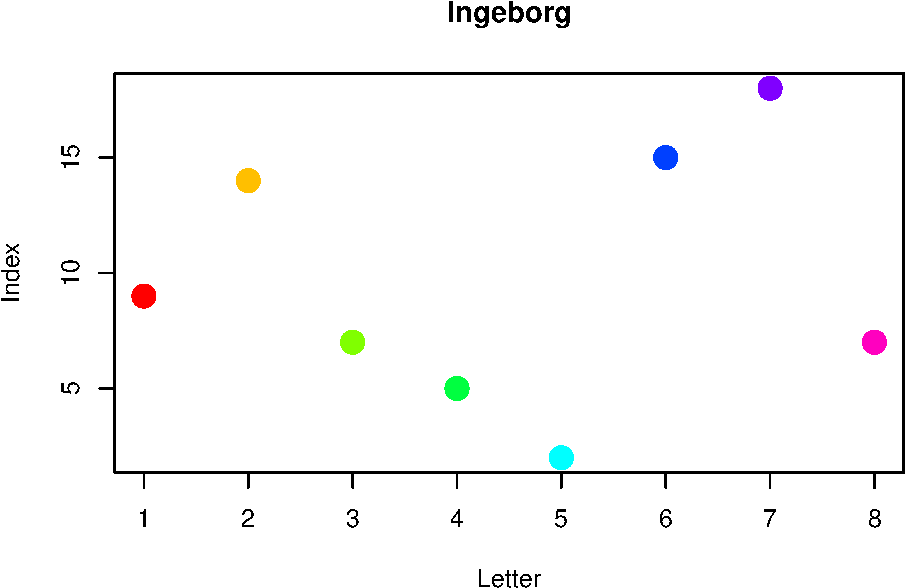
\includegraphics{2MLR_files/figure-latex/unnamed-chunk-61-1.pdf}

\begin{Shaded}
\begin{Highlighting}[]
\CommentTok{\# And a summary function}
\NormalTok{summary.test }\OtherTok{\textless{}{-}} \ControlFlowTok{function}\NormalTok{(obj) \{}

    \FunctionTok{cat}\NormalTok{(}\StringTok{"Word: "}\NormalTok{, obj}\SpecialCharTok{$}\NormalTok{word, }\StringTok{"}\SpecialCharTok{\textbackslash{}n}\StringTok{"}\NormalTok{)}
    \FunctionTok{cat}\NormalTok{(}\StringTok{"Length of word: "}\NormalTok{, }\FunctionTok{length}\NormalTok{(obj}\SpecialCharTok{$}\NormalTok{x), }\StringTok{" letters}\SpecialCharTok{\textbackslash{}n}\StringTok{"}\NormalTok{)}
    \FunctionTok{cat}\NormalTok{(}\StringTok{"Occurrence of each letter:"}\NormalTok{)}
    \FunctionTok{print}\NormalTok{(}\FunctionTok{table}\NormalTok{(}\FunctionTok{strsplit}\NormalTok{(}\FunctionTok{tolower}\NormalTok{(obj}\SpecialCharTok{$}\NormalTok{word), }\StringTok{""}\NormalTok{)))}

\NormalTok{\}}

\FunctionTok{summary}\NormalTok{(myname)}
\end{Highlighting}
\end{Shaded}

\begin{verbatim}
## Word:  Ingeborg 
## Length of word:  8  letters
## Occurrence of each letter:
## b e g i n o r 
## 1 1 2 1 1 1 1
\end{verbatim}

Now we have made a class with a plot, print and summary function, and
this is what you do in the exercise! But a bit more advanced\ldots{}

\begin{center}\rule{0.5\linewidth}{0.5pt}\end{center}

Let us look at what happens when we use the plotting function on objects
with different classes: The function called \texttt{plot}. First we make
two new objects that can be plotted:

\begin{Shaded}
\begin{Highlighting}[]
\NormalTok{data }\OtherTok{\textless{}{-}} \FunctionTok{data.frame}\NormalTok{(}\AttributeTok{x =} \FunctionTok{rnorm}\NormalTok{(}\DecValTok{10}\NormalTok{), }\AttributeTok{y =} \FunctionTok{rnorm}\NormalTok{(}\DecValTok{10}\NormalTok{))}
\NormalTok{mod }\OtherTok{\textless{}{-}} \FunctionTok{lm}\NormalTok{(y }\SpecialCharTok{\textasciitilde{}}\NormalTok{ x, }\AttributeTok{data =}\NormalTok{ data)}
\end{Highlighting}
\end{Shaded}

And then we plot them:

\begin{Shaded}
\begin{Highlighting}[]
\FunctionTok{plot}\NormalTok{(data)}
\end{Highlighting}
\end{Shaded}

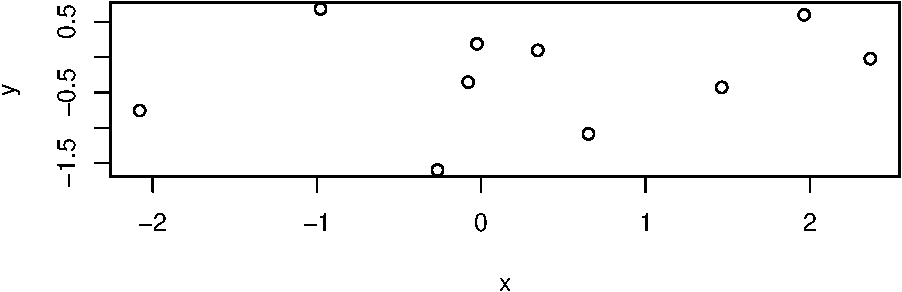
\includegraphics{2MLR_files/figure-latex/unnamed-chunk-64-1.pdf}

\begin{Shaded}
\begin{Highlighting}[]
\FunctionTok{plot}\NormalTok{(mod)}
\end{Highlighting}
\end{Shaded}

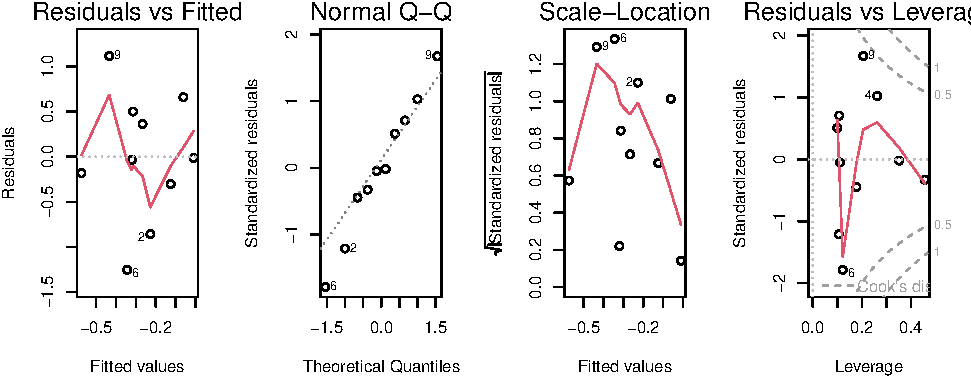
\includegraphics{2MLR_files/figure-latex/unnamed-chunk-64-2.pdf}

\begin{Shaded}
\begin{Highlighting}[]
\FunctionTok{plot}\NormalTok{(myname)}
\end{Highlighting}
\end{Shaded}

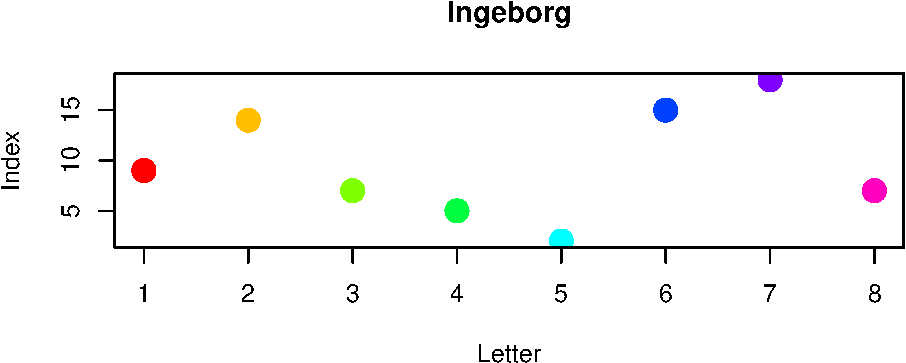
\includegraphics{2MLR_files/figure-latex/unnamed-chunk-64-3.pdf}

What is happening? \texttt{R} reads the class of the objects and uses
the plot-function made for that specific class. The user does not have
to specify the class as this is already stored in the object!

The different objects we have declared earlier have the following
classes:

\begin{Shaded}
\begin{Highlighting}[]
\FunctionTok{class}\NormalTok{(data)}
\FunctionTok{class}\NormalTok{(mod)}
\FunctionTok{class}\NormalTok{(myname)}
\end{Highlighting}
\end{Shaded}

\begin{verbatim}
## [1] "data.frame"
## [1] "lm"
## [1] "test"
\end{verbatim}

\begin{center}\rule{0.5\linewidth}{0.5pt}\end{center}

You will make a new class in \texttt{R} called \texttt{mylm}, and
\texttt{R} will also then understand which plot-function to use based on
the class.

Note that an object can have more than one class.

\begin{center}\rule{0.5\linewidth}{0.5pt}\end{center}

You write the report using R Markdown, use this template:
\url{https://www.math.ntnu.no/emner/TMA4315/2018h/template_glm.Rmd}

\begin{center}\rule{0.5\linewidth}{0.5pt}\end{center}

\hypertarget{exercises}{%
\paragraph{Exercises:}\label{exercises}}

Discuss with the group to get a feeling on what to do in the exercise.

\begin{enumerate}
\def\labelenumi{\arabic{enumi}.}
\tightlist
\item
  Go through how to make an R package together in the group, and make
  the mylm-package.
\item
  The core is the \texttt{mylm} function. Which formulas are used to

  \begin{itemize}
  \tightlist
  \item
    calculate parameters estimates?
  \item
    calculate covariance matrix of the estimated regression
    coefficients?
  \item
    perform type 3 hypothesis tests (remember you need to do the
    asymptotic normal - so no t-distributions)?
  \end{itemize}
\item
  You will make \texttt{print.mylm}, \texttt{plot.mylm} and
  \texttt{summary.mylm}. What should these functions contain?
\item
  Look at the mylm-template
  (\url{https://www.math.ntnu.no/emner/TMA4315/2018h/mylm.R}) and see if
  you understand it, or if you have questions about some of the parts.
  In particular, explore the functions \texttt{model.frame},
  \texttt{model.matrix} and \texttt{model.response}.
\end{enumerate}

\hypertarget{problem-4-munich-rent-index-optional}{%
\subsubsection{Problem 4: Munich Rent index
(optional)}\label{problem-4-munich-rent-index-optional}}

Last week all groups decided on using \texttt{rent} or \texttt{rentsqm}
as response, and in short - there was not really a big difference. So,
now use \texttt{rent} as the response.

\begin{enumerate}
\def\labelenumi{\arabic{enumi}.}
\tightlist
\item
  We now want to use model selection to arrive at a good model. Start by
  defining which covariates you want to include and how to code them
  (\texttt{location} as dummy or effect coding). What about year of
  construction - is that a linear covariate? Maybe you want to make
  intervals in time instead? Linear or categorical for the time? What
  about the \texttt{district}? We leave that since we have not talked
  about how to use spatial covariates.
\end{enumerate}

Hint: if you want to test out interval versions of year of construction
the function \texttt{mutate} (from \texttt{dplyr}) is useful:

\begin{Shaded}
\begin{Highlighting}[]
\NormalTok{rent99 }\OtherTok{\textless{}{-}}\NormalTok{ rent99 }\SpecialCharTok{\%\textgreater{}\%}
    \FunctionTok{mutate}\NormalTok{(}\AttributeTok{yearc.cat =} \FunctionTok{cut}\NormalTok{(yearc, }\AttributeTok{breaks =} \FunctionTok{c}\NormalTok{(}\SpecialCharTok{{-}}\ConstantTok{Inf}\NormalTok{, }\FunctionTok{seq}\NormalTok{(}\DecValTok{1920}\NormalTok{, }\DecValTok{2000}\NormalTok{, }\DecValTok{10}\NormalTok{)),}
        \AttributeTok{labels =} \DecValTok{10} \SpecialCharTok{*} \DecValTok{1}\SpecialCharTok{:}\DecValTok{9}\NormalTok{))}
\end{Highlighting}
\end{Shaded}

More on \texttt{dplyr}: Tutorial:
\url{http://genomicsclass.github.io/book/pages/dplyr_tutorial.html} and
Cheat sheet (data wrangling):
\url{https://www.rstudio.com/wp-content/uploads/2015/02/data-wrangling-cheatsheet.pdf}
and dplyr in particular:
\url{https://github.com/rstudio/cheatsheets/raw/master/source/pdfs/data-transformation-cheatsheet.pdf}

\begin{enumerate}
\def\labelenumi{\arabic{enumi}.}
\setcounter{enumi}{1}
\item
  There are many ways to perform model selection in MLR. One possibility
  is best subsets, which can be done using the \texttt{regsubsets}
  function from library \texttt{leaps}. You may define \texttt{x} from
  \texttt{model.matrix(fit){[},-1{]}} (not including the intercept
  term), and then run
  \texttt{best=regsubsets(x=model.matrix(fit){[},-1{]},y=rent99\$rent)}
  and look at \texttt{summary(best)}. Explain the print-out (with all
  the stars). Using the Mallows Cp (named \texttt{cp} in the list from
  \texttt{summary(best)}) will give the same result at using AIC (which
  is not available in this function). What is your preferred model?
  Hint: look at the R-code in Problem 2 (Figure 3) from the TMA4267V2017
  exam:
  \href{https://www.math.ntnu.no/emner/TMA4267/2017v/Exam/eV2017Enew.pdf}{pdf},
  and maybe the solutions for the interprtation
  \href{https://www.math.ntnu.no/emner/TMA4267/2017v/Exam/mergedLFV2017.pdf}{pdf}
\item
  Check what is done if you use \texttt{stepAIC}. Do you get the same
  model choice as with best subset selection based on AIC? Why, or why
  not?
\end{enumerate}

\begin{center}\rule{0.5\linewidth}{0.5pt}\end{center}

\hypertarget{quiz-with-kahoot}{%
\subsubsection{Quiz with Kahoot!}\label{quiz-with-kahoot}}

One person on each group go to \url{https://kahoot.it} on a mobile
device or a laptop. (The lecturer will hijack the screen for showing
questions so you it is difficult to use the PC.)

Give the pin (shown soon) and then give the team nick name
``Group1''-``Group8'' or make your own personalized group name. Then -
if you want - add nicks for all group members. Work together and only
provide \emph{one} answer to each question for each group. In team mode
there is a short ``team talk'' period before you can provide the answer
- so you have some time. 1000 points if you answer correctly
immediately, 500 if you answer when the time is up, 0 for wrong answers.

\hypertarget{wordclouds-are-cool}{%
\section{Wordclouds are cool?}\label{wordclouds-are-cool}}

Run the following code to make the wordcloud. The code can not be run by
\texttt{knit} because of how the graphics are made - so run and then you
need to save the resulting figure as a file (I choose png). Maybe you
want to run the code on another document? Please mail
\href{mailto:Mette.Langaas@ntnu.no}{\nolinkurl{Mette.Langaas@ntnu.no}}
if you do cool stuff for others to see!

\begin{Shaded}
\begin{Highlighting}[]
\FunctionTok{library}\NormalTok{(wordcloud2)}
\FunctionTok{library}\NormalTok{(tm)}
\NormalTok{all }\OtherTok{=} \FunctionTok{scan}\NormalTok{(}\StringTok{"https://www.math.ntnu.no/emner/TMA4315/2018h/2MLR.Rmd"}\NormalTok{, }\AttributeTok{what =} \StringTok{"s"}\NormalTok{)}

\NormalTok{corpus }\OtherTok{=} \FunctionTok{Corpus}\NormalTok{(}\FunctionTok{VectorSource}\NormalTok{(all))}
\NormalTok{corpus[[}\DecValTok{1}\NormalTok{]][}\DecValTok{1}\NormalTok{]}
\NormalTok{corpus }\OtherTok{=} \FunctionTok{tm\_map}\NormalTok{(corpus, }\FunctionTok{content\_transformer}\NormalTok{(tolower))}
\NormalTok{corpus }\OtherTok{=} \FunctionTok{tm\_map}\NormalTok{(corpus, removeNumbers)}
\NormalTok{corpus }\OtherTok{=} \FunctionTok{tm\_map}\NormalTok{(corpus, removeWords, }\FunctionTok{stopwords}\NormalTok{(}\StringTok{"english"}\NormalTok{))}
\NormalTok{corpus }\OtherTok{=} \FunctionTok{tm\_map}\NormalTok{(corpus, removeWords, }\FunctionTok{c}\NormalTok{(}\StringTok{"{-}{-}{-}"}\NormalTok{, }\StringTok{"bf"}\NormalTok{, }\StringTok{"boldsymbol"}\NormalTok{, }\StringTok{"will"}\NormalTok{,}
    \StringTok{"include"}\NormalTok{, }\StringTok{"use"}\NormalTok{, }\StringTok{"can"}\NormalTok{, }\StringTok{"follow"}\NormalTok{, }\StringTok{"provide"}\NormalTok{, }\StringTok{"using"}\NormalTok{))}
\NormalTok{corpus }\OtherTok{=} \FunctionTok{tm\_map}\NormalTok{(corpus, removePunctuation)}
\NormalTok{corpus }\OtherTok{=} \FunctionTok{tm\_map}\NormalTok{(corpus, stripWhitespace)}
\CommentTok{\# corpus=tm\_map(corpus,stemDocument)}

\NormalTok{tdm }\OtherTok{=} \FunctionTok{TermDocumentMatrix}\NormalTok{(corpus)}
\NormalTok{m }\OtherTok{=} \FunctionTok{as.matrix}\NormalTok{(tdm)}
\NormalTok{v }\OtherTok{=} \FunctionTok{sort}\NormalTok{(}\FunctionTok{rowSums}\NormalTok{(m), }\AttributeTok{decreasing =} \ConstantTok{TRUE}\NormalTok{)}
\NormalTok{d }\OtherTok{=} \FunctionTok{data.frame}\NormalTok{(}\AttributeTok{word =} \FunctionTok{names}\NormalTok{(v), }\AttributeTok{freq =}\NormalTok{ v)}
\FunctionTok{dim}\NormalTok{(d)}
\NormalTok{d[}\DecValTok{1}\SpecialCharTok{:}\DecValTok{10}\NormalTok{, ]}
\FunctionTok{wordcloud2}\NormalTok{(d, }\AttributeTok{shape =} \StringTok{"cardioid"}\NormalTok{, }\AttributeTok{maxRotation =}\NormalTok{ pi}\SpecialCharTok{/}\DecValTok{10}\NormalTok{, }\AttributeTok{minRotation =} \SpecialCharTok{{-}}\NormalTok{pi}\SpecialCharTok{/}\DecValTok{10}\NormalTok{)}
\end{Highlighting}
\end{Shaded}

\includegraphics{./M2wordcloud.png}

\hypertarget{r-packages}{%
\section{R packages}\label{r-packages}}

\begin{Shaded}
\begin{Highlighting}[]
\FunctionTok{install.packages}\NormalTok{(}\FunctionTok{c}\NormalTok{(}\StringTok{"formatR"}\NormalTok{, }\StringTok{"gamlss.data"}\NormalTok{, }\StringTok{"tidyverse"}\NormalTok{, }\StringTok{"ggplot2"}\NormalTok{,}
    \StringTok{"GGally"}\NormalTok{, }\StringTok{"Matrix"}\NormalTok{, }\StringTok{"nortest"}\NormalTok{, }\StringTok{"lmtest"}\NormalTok{, }\StringTok{"wordcloud2"}\NormalTok{, }\StringTok{"tm"}\NormalTok{))}
\end{Highlighting}
\end{Shaded}

\hypertarget{references-and-further-reading}{%
\section{References and further
reading}\label{references-and-further-reading}}

\begin{itemize}
\tightlist
\item
  Slightly different presentation (more focus on multivariate normal
  theory):
  \href{https://www.math.ntnu.no/emner/TMA4267/2017v/TMA4267V2017Part2.pdf}{Slides
  and written material from TMA4267 Linear Statistical Models in 2017,
  Part 2: Regression (by Mette Langaas).}
\item
  And, same source, but now {[}Slides and written material from TMA4267
  Linear Statistical Models in 2017, Part 3: Hypothesis testing and
  ANOVA{]}
  (\url{http://www.math.ntnu.no/emner/TMA4267/2017v/TMA4267V2017Part3.pdf})
\end{itemize}

\end{document}
